\documentclass[a4paper,oneside]{report}

%%%
%%% Para insertar imágenes
%%%
\usepackage[pdftex]{graphicx}

%%%
%%% Nombres de secciones y demás en castellano
%%%
\usepackage[spanish]{babel}


%%%
%%% Permite introducir caracteres castellanos
%%%
\usepackage[utf8]{inputenc}

\usepackage{float}
\usepackage[pdfborder={0 0 0}]{hyperref}
%%%%%%
%% Añade un marco a las imágenes
%%%%%%
\floatstyle{boxed}
\restylefloat{figure}



%%%
%%%  Márgenes de las hojas
%%%
\usepackage[top=2cm, bottom=1.25in, left=2cm, right=2cm]{geometry}


\newcommand{\HRule}{\rule{\linewidth}{0.5mm}}
%%\usepackage{listings}


%%%
%%%  Insertar una imagen rápidamente
%%%
\newcommand{\figura}[3]{
	\begin{figure}[H]
		\includegraphics[width=\textwidth]{#1}
		\caption{#2}
		\label{#3}
	\end{figure}
}

%\newcommand{\figuraCap}[4]{
%	\begin{figure}[H]
%		\includegraphics[width=\textwidth]{#1}
%		\caption{[#2]#3}
%		\label{#4}
%	\end{figure}
%}



%%%
%%%   Datos
%%%
\title{OpenERP - Guía de usuario}

\author{Sicnova 3D Murcia}



%%%%%%%%%%%%%%%%%%%%%%%%%%%%%%%%%%%
%%%%%%%%%%%%%%%%%%%%%%%%%%%%%%%%%%%
%%%%%%%%%%%%%%%%%%%%%%%%%%%%%%%%%%%

\begin{document}


%%%
%%%  Portada
%%%
\begin{titlepage}
\begin{center}

% Upper part of the page. The '~' is needed because \\
% only works if a paragraph has started.
%\includegraphics[width=0.15\textwidth]{./logo}\\[1cm]
\vspace*{5cm}
\textsc{\LARGE Sicnova 3D}\\[1.5cm]

\textsc{\Large Manual de uso}\\[0.5cm]

% Title
\HRule \\[0.4cm]
{ \huge \bfseries Manual de usuario de OpenERP \\[0.4cm] }

\HRule \\[1.5cm]

% Author and supervisor
\noindent
\vfill
\begin{minipage}{0.4\textwidth}
\begin{flushleft} \large
\emph{Autor}\\
%Sicnova 3D Murcia
Filé Aesir
\end{flushleft}
\end{minipage}%
\begin{minipage}{0.4\textwidth}
\begin{flushright} \large
\emph{Versión} \\
0.3
\end{flushright}
\end{minipage}
\vspace{2cm}


% Bottom of the page
%{\large \today}[width=\textwidth]\\

\includegraphics[width=2cm]{GFDL.png}\\
GNU Free Documentation License v1.3\\
Copyright \copyright 2014 Filé Aesir -- Gabriel Franco

\end{center}
\end{titlepage}



%\maketitle
%%%
%%%  Aviso licencia
%%%
\begin{flushright}

\vspace*{4cm}

%\begin{verbatim}

\begin{tabular}{r l}
	Copyright \copyright 2014  & Gabriel Franco $<$gabriel.franco.martinez@gmail.com$>$\\
	Copyright \copyright 2014 & Filé Aesir $<$file@fileaesir.com$>$\\
\end{tabular}\\[1cm]

    Permission is granted to copy, distribute and/or modify this document\\
    under the terms of the GNU Free Documentation License, Version 1.3\\
    or any later version published by the Free Software Foundation;\\
    with on Invariant Section: "Sobre este documento", no Front-Cover Texts,\\
    and no Back-Cover Texts. A copy of the license is included in the\\
    section entitled "GNU Free Documentation License".\\[1cm]


    Se garantiza el permiso para copiar, distribuir y/o modificar este documento\\
bajo los terminos de la Licencia GNU Free Documentation, Versión 1.3\\
o cualquier otra versión posterior publicada por la Free Software Foundation;\\
con una Sección Invariante: "Sobre este documento", sin textos de portada y sin\\
textos de contraportada. Una copia de esta licencia se incluye en la sección \\
titulada "GNU Free Documentation License".
%\end{verbatim}

\end{flushright}



\tableofcontents



%\include{general/general}

%%
% Este archivo es parte de un documento sobre OpenERP/Odoo creado
% y distribuido bajo licencia GNU Free Documen License v1.3.
%
% Para obtener la fuente e información más detallada, visite
% https://github.com/Gabriel-fm/oerp-manual
%
% Copyright (c) 2014 - Gabriel Franco
%

\chapter{Productos}
\label{productos}
Los productos y sus fichas son accesibles desde distintos puntos de la aplicación. También, según desde el punto en el que se acceda, se le acompañará un menú u otro para modificar categorias u otros elementos. Se verá cada una de estas opciones a continuación y se especificará como acceder a las mismas.

En primer lugar se analiza la ficha de los productos y sus distintas pestañas.

\section{Ficha de producto}

En la figura \ref{pro:ficha} se puede observar la vista de la ficha. En esta se puede apreciar un área con distinas pestañas para la diversa información del producto y un área superior, más pequeña, que será fija y que contendrá menos opciones.

En este área superior es donde se introducirá el \textbf{Nombre del producto} y bajo el mismo se puede especificar la \textbf{Categoría} a la que pertenece dicho producto. Una explicación más detallada sobre las categorías se da en la sección \ref{pro:categorias}.

\figura{productos/img/pro_ficha.png}
{Visión principal de una ficha}
{pro:ficha}

Bajo el nombre y la categoría aparecen las opciones \textbf{Puede ser vendido} y \textbf{Puede ser comprado}. La selección de cada uno de ellos, permitirá que estos productos se puedan añadir a líneas de presupuestos, pedidos de venta y documentos de venta en genral, y/o a líneas de compras respectivamente. El caso típico son los productos que se utilizan para construir/fabricar los productos que se van a vender. Estos productos, equivalentes a materias primas, tendrán marcada la opción de venta, no de compra. Con esta selección se podrán comprar esas \emph{materias primas}, pero no podrán venderse, evitando así errores e inflar la lista de productos de venta.

En la parte superior derecha de este área general, se observan dos botones: \textbf{Pedir abastecimiento} y \textbf{Puntos de pedidos}. A través del primer botón lo que se hará es solicitar el abastecimiento del producto en el almacén indicado -- puede verse la ventana emergente que aparece al hacer click sobre este botón en la figura \ref{pro:pedirAbastecimiento}. Para este pedido puede especificarse el almacén donde se recibirá/guardará -- que muestra el \textbf{Almacén} por defecto del producto según las configuraciones que se verán después, la \textbf{Cantidad} de productos a abastecer. La \textbf{Fecha prevista} es calculada a partir de los datos del producto, aunque cabe la posibilidad de variarla en este menú.

Con el botón \textbf{Puntos de pedidos} se mostrará un listado de las ordenes de reabastecimiento (y se podrán crear aquí también) tal como se describe en la sección \ref{alm:reabastecimiento}

\figura{productos/img/pro_pedirAbastecimiento.png}
{Diálogo para solicitar abastecimiento de un producto}
{pro:pedirAbastecimiento}

\subsection{Pestaña de Información}
Esta pestaña se puede ver en la figura \ref{pro:ficha} de la sección anterior. En este caso hay unas pocas opciones que se ennumeran a continuación:

\begin{itemize}
  \item \textbf{Tipo de producto} -- Indica que tipo de producto es, siempre en relación con su posibilidad de stockage, por defecto:
    \begin{itemize}
      \item \textbf{Almacenable} -- Permitirá hacer un seguimiento del stock de este producto
      \item \textbf{Servicio} y \textbf{Consumible} -- Para este caso no hará diferenciación en cuanto al stock -- no se hará un 
                   seguimiento. La diferencia aquí estriba en que define si el producto es físico o es un servicio.
     \end{itemize}
  \item \textbf{Precio de venta} -- Precio de catálogo, es el que será de venta para los clientes.
  \item \textbf{Referencia interna} -- Código de referencia de uso interno en la empresa.
  \item \textbf{Código EAN13} -- Código EAN13 internacional, el código de barras usualmente.
\end{itemize}

También existe un área de notas en la zona inferior que permite insertar texto descriptivo sobre el producto ya sean anotaciones o descripción de sus caracteristicas.


\subsection{Pestaña de Abastecimientos}

En esta pestaña se encontrará la información relativa a como se obtiene el producto desde el proveedor hasta la empresa. Existen distintas opciones. Para empezar, hay que puntualizar que son el \textbf{Método de abastecimiento} y el \textbf{Método de suministro}

\figura{productos/img/pro_pesAbastecimiento.png}
{Pestaña de Abastecimiento de un producto}
{pro:pesAbastecimiento}

El \textbf{Método de abastecimiento} puntualizará que se hará cuando el producto se añada en una línea de venta, señalará \textbf{cómo} se obtendrá el producto, por parte de la empresa, \textbf{para el envío al cliente}. Las dos opciones disponibles son:

\begin{itemize}
  \item \textbf{Obtener desde stock} -- Cuando un producto que tiene seleccionada esta opción, se añade a una línea de venta, el producto
               se obtendrá del stock del almacén. En el caso de que no haya stock en el almacén, el encargado de almacén se encargará de
               poner el producto en disposición par ael envío y, si no hubiera producto en stock, el encargado deberá crear la orden de
               compra del mismo
  \item \textbf{Obtener desde pedido} -- Al añadir en una línea de compra un producto marcado con esta opción, lo que se hará es crear
               automáticamente la orden de compra del mismo (o la orden de fabricación) independientemente del stock. 
\end{itemize}

El \textbf{Método de suministro} indicará \textbf{cómo} se obtendrá el producto desde el proveedor a la empresa, sin tener en consideración al cliente. Las dos opciones son:

\begin{itemize}
  \item \textbf{Fabricar} -- Cuando se vaya a obtener stock para el producto, lo que se va a hacer es fabricarlo.
  \item \textbf{Comprar} -- Para obtener el stock del producto, se compra el mismo sin necesidad de fabricarlo, a un proveedor.
\end{itemize}

Se ha de notar que estas dos opciones son totalmente complementarias. La primera está relacionada con cómo se sirve el producto ante un pedido y el segundo se relaciona a cómo se obtiene el producto (independientemente de si existe un pedido o no)

El \textbf{Precio de coste} que aparece a continuación es el precio del producto a la hora de comprarlo, se utiliza como precio base en los pedidos de compras.

Junto a \textbf{Retrasos} aparece el campo \textbf{Plazo de entrega de fabricación}. En este se introduce el tiempo (en días) necesario para producir -- cuanso se fabrica -- el producto.

La opción \textbf{Activo} indica si el producto está activo o no. En el caso de que no lo esté, no aparecerá en las busquedas ni desplegables para ser insertado en líneas de pedidos (tanto de compras como de ventas). Siempre puede buscarse a través de la pantalla de \emph{Productos} y cambiar esta opción.

El área inferior está dedicada a los \textbf{Proveedores}. Abajo del todo existe un área de texto donde introducir notas que se insertarán automáticamente en las solicitudes de presupuesto a los proveedores. Encima se encuentra la lista de proveedores para este producto. Se pueden añadir tantos como sea necesario, para cada uno que se añada desde aquí aparecerá una ventan flotante para la inserción de sus datos (figura \ref{pro:addProveedor})

\figura{productos/img/pro_addProveedor.png}
{Ventana para crear un Proveedor}
{pro:addProveedor}

El campo \textbf{Proveedor} se utiliza para marcar que empresa (añadida anteriormente o que es posible crear insitu) se utilizará como proveedor de este producto. El campo \textbf{Nombre producto proveedor} permite añadir un nombre personalizado para este producto en el proveedor dado de manera que aparezca en los presupuestos de compra con el nombre adecuado según a quién se dirija. De igual forma se utiliza el campo \textbf{Código producto proveedor}, pudiendo personalizar el código del mismo en función de a quién se realice el pedido.

La \textbf{Cantidad mínima} representa cuál es la cantidad mínima de compra del producto en el distribuidor. De igual forma el \textbf{Tiempo de entrega} señala cuantos días, desde el momento de confirmación de recepción del pedido por parte del proveedor, se tarda en ser entregado a la empresa.

El último campo a señalar es \textbf{Secuencia}. Este indica la prioridad del proveedor en la lista de todos los proveedores. A numeración menor (más cercana a 1) más arriba se encontrará en la lista de proveedores, y cuanto más se acerque a 10, más al final se encontrará.





\subsection{Pestaña de Inventario}

\figura{productos/img/pro_pesInventario.png}
{Pestaña de Inventario de productos}
{pro:pesInventario}

La figura \ref{pro:pesInventario} se observan todos los campos disponibles en la pestaña \textbf{Inventario} de las fichas de los productos divididas en varias secciones.

La parte \textbf{Existencias y variaciones esperadas} muestra información sobre el stock del producto en los almacenes de la empresa. 

\begin{itemize}

  \item \textbf{Stock real} -- Muestra el stock del producto que existen físicamente en el almacén.
  \item \textbf{Entrante} -- Número de items del producto que se esperen que entren en stock, que se encuentran pedidos pero no se encuentran físicamente aún en almacén.
  \item \textbf{Saliente} -- Cantidad de productos a los que se les va a dar salida. Es el número de items de este producto que se encuentran en líneas de ventas que aún no se han servido desde el almacén.
  \item \textbf{Stock virtual} -- Es el resultado de combinar todos los anteriores, es la cantidad prevista de stock de este producto cuando se terminen los pedidos de compra y de venta. En este caso, este número representa: Stock real - Saliente + Entrante

\end{itemize}


El \textbf{Estado} indica como se encuentra este producto en su ciclo de vida, de manera que se puede informar a aquel que esté viendo la ficha sobre si este producto es estable o no (si está en desarrollo) o si debe intentar evitar venderlo (Fin de ciclo de vida) o lo que se consensue a nivel de empresa para cada uno de estos valores. Se puede elegir entre las siguientes propiedades:

\begin{itemize}
\item En desarrollo
\item Normal
\item Fin de ciclo de vida
\item Obsoleto
\end{itemize}

De igual forma, el \textbf{Responsable de producto} representa el usuario (a nivel interno de la empresa) que se encarga del producto.

La zona de \textbf{Ubicación de almacenamiento} da una serie de campos que sirve para indicar la localización física del stock de este producto en el almacén, pudiendo indicar el \emph{estante}, la \emph{fila} y la \emph{caja}

El área de \textbf{Pesos} sirve para indicar el \textbf{Volumen} del producto (en $m^3$), su \textbf{Peso bruto} medido en Kg.y su \textbf{Peso neto} también en Kg.

Las \textbf{Propiedades de las ubicaciones parte recíproca} permite especificar las ubicaciones para el producto dentro del almacén. Para más información sobre estos campos y su significado, ver la sección \ref{moduloAlmacen}





\subsection{Pestaña de Ventas}

Esta pestaña permite afinar ciertos datos sobre las condiciones de venta del producto. La pestaña se puede ver íntegra en la figura \ref{pro:pesVentas} 

\figura{productos/img/pro_pesVentas.png}
{Captura de la pestaña \emph{Ventas} de la ficha de productos}
{pro:pesVentas}

La \textbf{Garantía} es expresada en meses y el \textbf{Plazo de entrega al cliente} se mide en días.

El listado inferior permite introducir información sobre el empaquetamiento del producto. Se pueden insertar tantas líneas como sean necesarias según como se encuentre empaquetado el producto, identificando cada una de estas \emph{unidades logísticas} por su código EAN. La información que se añade en cada una de estas líneas de unidades logísticas se ve en la figura \ref{pro:addPaquete}.

\figura{productos/img/pro_addPaquete.png}
{Diálogo para añadir información sobre paquetes}
{pro:addPaquete}

El campo \textbf{EAN} permite introducir el código identificatorio de esta forma de empaquetamiento. La \textbf{Cantidad por paquete} indica el \emph{número total} de productos que se encontraran en este empaquetamiento, y el \textbf{Peso paquete vacío} indica el peso del paquete sin tener en cuenta el peso de los productos introducidos en el mismo. El \textbf{Tipo de empaquetado} indica y describe como es el paquete, hay más detalle sobre estos elementos en la sección \ref{pro:empaquetado}.

La \textbf{paletización} se utiliza para indicar la organización interna del paquete. El \textbf{Número de capas} señala cuantas capas de productos se encontrarán en el paquete, los \textbf{Paquetes por piso} indican el total de productos en cada capa del paquete y el \textbf{Total peso paquete} sirve para indicar en Kg. el peso total del paquete con los productos dentro incluidos.

Las \textbf{Dimensiones del palet} se dan en metros y van a dar la información sobre la geometría externa del producto ya empaquetado.

En el campo \textbf{Descripción} se pueden dar detalles sobre el empaquetado que sea necesario puntualizar.


Volviendo a la \emph{Pestaña de ventas}, un último campo a destacar es el de \textbf{Descripción para las ofertas}, que son notas que se añadirán a posteriori en los presupuestos de venta. Puede servir para puntualizar detalles sobre la garantía o detalles en el proceso de venta.




\subsection{Pestaña de Contabilidad}
\figura{productos/img/pro_pesContabilidad.png}
{Pestaña de información sobre la contabilidad de un producto}
{pro:pesContabilidad}

En esta pestaña se introducirá la información relativa al tratamiento contable de los movimientos realizados con el producto. Esta pestaña tan solo tiene 4 campos (figura \ref{pro:pesContabilidad})

Dos de los campos son \textbf{Cuenta de ingresos} y \textbf{Cuenta de gastos} que indican a que cuentas se hará referencia en los apuntes y asientos contables cuando haya movimientos relacionados con este producto. Pueden dejarse las cuentas por defecto -- que serán las genéricas -- o bien se pueden utilizar subcuentas para controlar los gastos e ingresos de cada producto.

Los campos \textbf{Impuestos cliente} e \textbf{Impuestos proveedor} sirven para introducir los impuestos por defecto para estos productos. El tener estos impuestos configurados aquí, hace que al añadir el producto en una línea de venta o de compra, añada automáticamente el impuesto relacionado, evitando el tener que introducir los impuestos de cada producto cada vez que son añadidos en una transacción.





\section{Categorías de productos}
\label{pro:categorias}

Los productos se pueden clasificar en \textbf{categorías} las cuales pueden organizarse en forma de árbol tal y como se aprecia en la figura \ref{pro:listaCategorias}. En esa misma figura se aprecia como se muestran las categorías y el árbol de categorías. Aquellas en las que en su nombre aparece la barra inclinada $/$ indican la ruta en el árbol de categorías, siendo el elemento a la izquierda de la barra padre del elemento a la derecha.

\figura{productos/img/pro_categorias.png}
{Listado de categorías de productos}
{pro:listaCategorias}

Las propiedades de las categorías se pueden observar al pulsar sobre ellas, mostrando de esa manera la ficha individual de la categoría. Un ejemplo es el que se aprecia en la figura \ref{pro:crearCategoria}

\figura{productos/img/pro_crearCategoria.png}
{Datos de una categoría}
{pro:crearCategoria}


El \textbf{Nombre} será el identificador de la categoría, y la \textbf{Categoría padre} será una categoría ya existente previamente, que convertirá la categoría en edición en hija de la indicada en tal campo. El \textbf{tipo de categoría} indica que tipo de categoría es, pudiendo elegir entre dos tipos:

\begin{itemize}
  \item \textbf{Normal} -- Una categoría normal que puede incluir productos dentro de la misma.
  \item \textbf{Vista} -- Es una categoría especial que no contendrá productos, pero si más categorías. Es un tipo de categoría orientada a la organización de la estructura del árbol de categorías.
\end{itemize}

Las \textbf{Propiedades de la cuenta} actuan de igual manera que las cuentas que aparecían en la pestaña de contabilidad del producto. Todos los productos qaue caigan en el interior de dicha categoría, apuntarán sus movimientos contables dentro de las cuentas indicadas en función de si es un movimiento de venta o de compra. A menos que los productos que estén en esta categoría tengan sus propios datos sobre las cuentas contables, se utilizarán los indicados aquí.

Las \textbf{Cuenta de entrada de existencias}, \textbf{Cuenta de salida de existencias}, \textbf{Cuenta de valoración de existencias} y \textbf{Diario de existencias} son las cuentas, a nivel de stock en las que se apuntarán los movimientos de stock de los productos de esta categoría (para más detalle sobre esto, ver la sección \ref{moduloAlmacen}.





\section{Empaquetado}
\label{pro:empaquetado}

La pantalla de \textbf{empaquetado} es accesible como una opción del menú desplegable \emph{Productos} en el área de \emph{Configuración} de la barra de opciones de la izquierda. Es accesible sólo cuando se tienen los permisos adecuados.

Al acceder a esta opción, se presenta un listado de tipos de paquete como se ve en la figura \ref{pro:paquete}. Cada uno de estos elementos es accesible haciendo click sobre los mismos, presentando la configuración de los mismos, consistente en dos opciones tal y como se observa en la figura \ref{pro:paqIndividual}

\figura{productos/img/pro_paquete.png}
{Listado de paquetes disponibles}
{pro:paquete}

\figura{productos/img/pro_paqIndividual.png}
{Configuración de los datos de un paquete}
{pro:paqIndividual}

Las opciones configurables son el \textbf{Nombre}, que sirve a la vez como descripción del paquete como se ve en las figuras anteriores, y el \textbf{Tipo} de empaquetado. El tipo permite elegir entre las siguientes opciones:

\begin{itemize}
\item Unidad
\item Paquete
\item Caja
\item Palet
\end{itemize}

A pesar de una apariencia de pocas opciones y utilidad, definir de esta manera el empaquetamiento sirve para que, cuando se configuren los productos, los tamaños según paquetes, palets u otro tipo de empaquetamiento esté estandarizado y no quepa lugar a error o a utilizar empaquetamientos no disponibles o no estandarizados por la empresa.


%\section{Unidades de medida}
%\subsection{Categorías de unidades de medida}


%
% Este archivo es parte de un documento sobre OpenERP/Odoo creado
% y distribuido bajo licencia GNU Free Documen License v1.3.
%
% Para obtener la fuente e información más detallada, visite
% https://github.com/Gabriel-fm/oerp-manual
%
% Copyright (c) 2014 - Gabriel Franco
%

\chapter{Módulo de ventas}


%\section{Conceptos generales}

\section{Ventas}

La sección de ventas dentro del módulo de mismo nombre, es la sección a través de la 
cual se hará el seguimiento y control de las ventas de productos. Esto incluye tanto
las ventas probables como las ventas reales.

La estructuración de los menus sirves para tener una visión escalonada del punto en el que
se encuentra una posible venta. Cuando aparece una posible venta, según su origen (se verá
después) aparecerá un nuevo elemento en \textbf{Iniciativas} o \textbf{Oportunidades}. En
este punto se trata de un contacto con un posible cliente con el cuál se le va a dar forma a
la venta. En este punto aún no hay nada acordado con el mismo y sólo indica la existencia
de esa probable venta.

Cuando se ha tratado lo suficiente con el cliente y se ha dado forma a una oferta en la que el
cliente está interesado, el elemento creado en el apartado anterior (\emph{Iniciativas} o
\emph{ventas}) se escalará y pasará a formar un \textbf{Presupuesto} que se enviará al cliente
para su aprobación. En este punto se habla de una venta probable a falta de la aprobación del
cliente.

Si el presupuesto es aprobado, este pasará (escalandose, igual que anteriormente) a convertirse
en un \textbf{Pedido de venta}, el cuál es un elemento que permitirá al comercial al cargo
\emph{confirmar la venta} de un presupuesto, \emph{generar una factura} como en el apartado
\ref{contabilidad:factura} (que deberá ser aprobada por alguien
encargado de facturación) y \emph{generar un pedido de envío} en almacén (que será aprobado y
 gestionado por el encargado de almacén) que se puede ver en el la sección \ref{almacen:envio}.


\subsection{Clientes}
\label{ven:clientes}
Esta sección es el punto principal de acceso a los datos sobre los clientes. Al hacer click
sobre el mismo aparecerá el listado de clientes en su vista Kanban. En esta vista de datos
se pueden ver de un vistazo el nombre, datos de la empresa, correos, etiquetas y 
enlaces a las posibles oportunidades y ventas de los clientes. La figura \ref{ven:clikanban}
muestra la visión kanban. En los recuadros azules se pueden observar las etiquetas
y en algunos de ellos, bajo el nombre y/o las etiquetas se aprecian los enlaces a 
las oportunidades y ventas.

\begin{figure}[H]
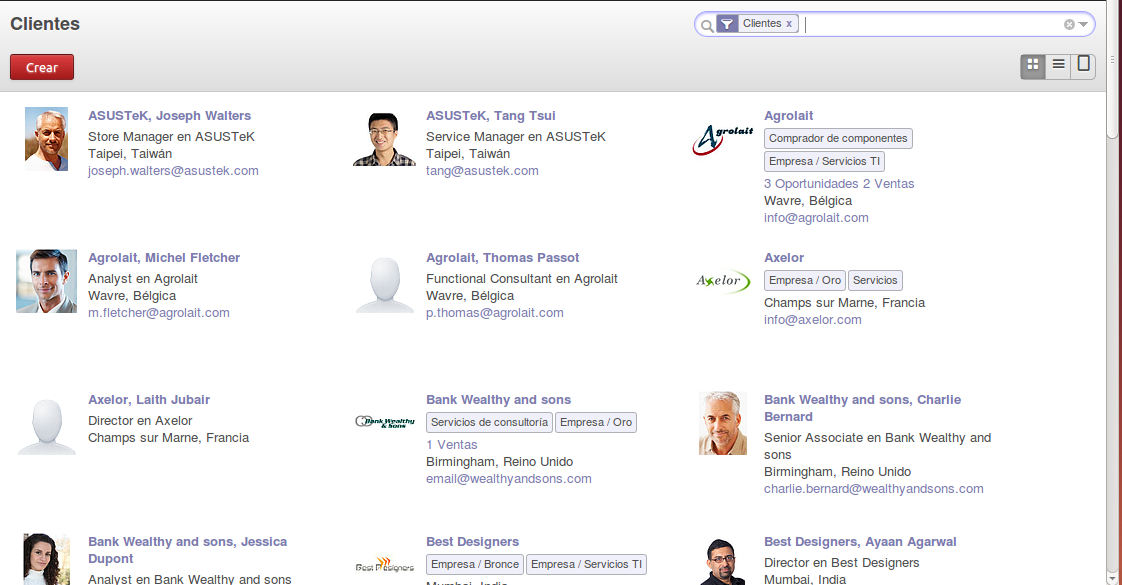
\includegraphics[width=\textwidth]{ventas/img/ven_clikanban.png}
\caption{Vista Kanban de clientes}
\label{ven:clikanban}
\end{figure}

Seleccionar uno de los clientes abrirá la ficha del mismo, pudiendo ver los datos del 
cliente que no estaban a la vista en la visión reducida. Esta ficha se compone de una
parte con los datos más "comunes" de los clientes y una serie de pestañas con información
adicional (contabilidad, ventas\ldots) sobre el mismo. La parte común se puede observar a
continuación en la figura \ref{ven:cliindividual}

\figura{ventas/img/ven_cliindividual.png}
{Información básica en la ficha de cliente}
{ven:cliindividual}


La mayoría de los campos son suficientemente autodescriptivos. Es necesario
mencionar otros no tan intuitivos. Por ejemplo, el cuadro de chequeo \textbf{¿Es una empresa?}
es utilizado para indicar si los datos que se están rellenado son de una empresa o 
de una persona en particular. Cuando este cuadro está marcado, se pueden crear nuevos
clientes y asociarlos a esta empresa. Para ello, los clientes que forman parte de esa
empresa, no tendrán marcado este cuadro de selección. Cuando este cuadro no se encuentra
seleccionado, aparece un nuevo campo que se denomina \emph{Compañia}, donde se indica
la compañia a la que pertenece el contacto.

Creando el contacto de la empresa y los contactos de personas relacionados con la misma
se consigue, por un lado, que la información de facturación y envío sea la de la empresa, 
evitando tener que rellenar varias veces la misma información en distintas fichas. Por otro
lado se organiza la información para que desde la ficha de la empresa se puedan observar también
los contactos que pertenecen a la misma, además de agilizar a la hora de realizar busquedas
el tener organizados los contactos con sus empresas.

En el área superior derecha se encuentran una serie de botones que permiten acceder a las reuniones, llamadas,
oportunidades y presupuestos y pedidos de compra de los clientes, presentando la lista de los elementos seleccionados
exclusivamente del cliente.

El área de \textbf{etiquetas} se utiliza para añadir identificadores a los clientes. Se utilizan
palabras cortas que identifiquen el área de trabajo de la empresa. Para clientes y empresas
que trabajen en joyería se debe añadir a los mismos la etiqueta \emph{joyería}, por ejemplo. La idea
es organizar todos los contactos con distintas etiquetas. Organizarlo de esta manera
optimiza los resultados a la hora de realizar busquedas.

En cuanto a las pestañas de la ficha de cliente se organizan en:

\subsubsection{Pestaña de Contactos}
En esta pestaña se pueden crear nuevos contactos que serán asociados directamente a la
empresa de la ficha. Si se crean nuevos contactos (en otro lugar, fuera de esta pestaña)
y se le asigna una compañia, esos contactos aparecerán aquí directamente.


\subsubsection{Pestaña de Notas Internas}
Permite almacenar información sobre el contacto, se guarda como texto en plano.


%\subsubsection{Pestaña de Información Mercantil}
\subsubsection{Pestaña de Ventas y Compras}
La información de esta pestaña es relativa a la información necesaria para realizar el contacto
con el cliente.

\begin{figure}[H]
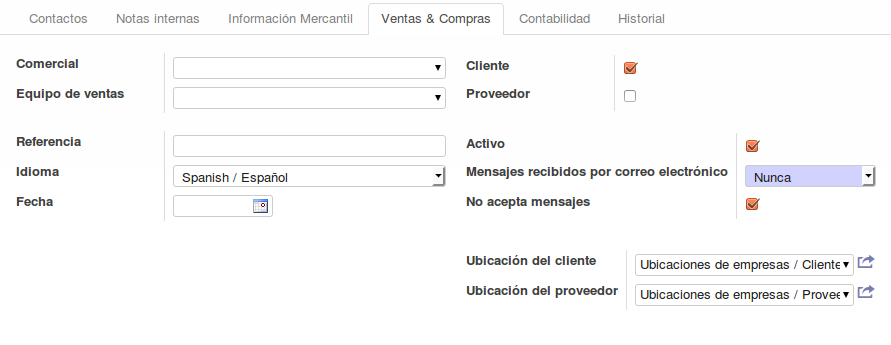
\includegraphics[width=\textwidth]{ventas/img/ven_cliventas.png}
\caption{Pestaña de Ventas y Compras en la ficha del cliente}
\label{ven:cliventas}
\end{figure}

\begin{itemize}
  \item \textbf{Comercial} -- Comercial al que se encuentra asignado este cliente
  \item \textbf{Equipo de ventas} -- Equipo de ventas en el que está asignado el cliente.
  \item \textbf{Referencia} -- Si se utiliza algún tipo de referencia a los clientes
        este campo es el lugar para ponerlo.
  \item \textbf{Idioma} -- Idioma del cliente. Según el idioma elegido, se enviarán los correos automáticos
        en el elegido.
  \item \textbf{Fecha} -- Permite almacenar una fecha. Según las necesidades del usuario.
  \item \textbf{Cliente/Proveedor} -- Según lo seleccionado en estos campos, se interpretará la información
        del contacto como un cliente o un proveedor. No es excluyente, es posible que los contactos sean
        proveedores y clientes al mismo tiempo.
  \item \textbf{Activo} -- Indica si el cliente/proveedor está activo. Si no seencuentra activo
        la información está almacenada, pero no se mostrará el cliente a menos que se busque de manera más
        específica.
  \item \textbf{No acepta mensajes} -- Indicador de si el cliente desea o no recibir correos.
  \item \textbf{Ubicaciones} -- Si se utilizan ubicaciones específicas en almacen para los datos de este cliente
        han de especificarse aquí.
\end{itemize}


\subsubsection{Pestaña de Contabilidad}
Los datos específicos sobre contabilidad del cliente se almacenan en esta pestaña.

Los distintos campos son autoexplicativos aunque cabe recalcar que la información del NIF debe introducirse
\textbf{en formato europeo}, es decir, con el prefijo de dos letras del país, la letra del NIF y el número. Para un NIF
español el formato sería con el prefijo ES de España, por ejemplo: ESA43683955 

Si al cobrar a un cliente se quiere almacenar la información de la transacción en un cuenta de contabilidad
43 específica, debe añadirse aquí (por ejemplo, para el primer cliente la cuenta sería 43000001)
De igual manera se trata la \emph{Cuenta a pagar}.

\begin{figure}[H]
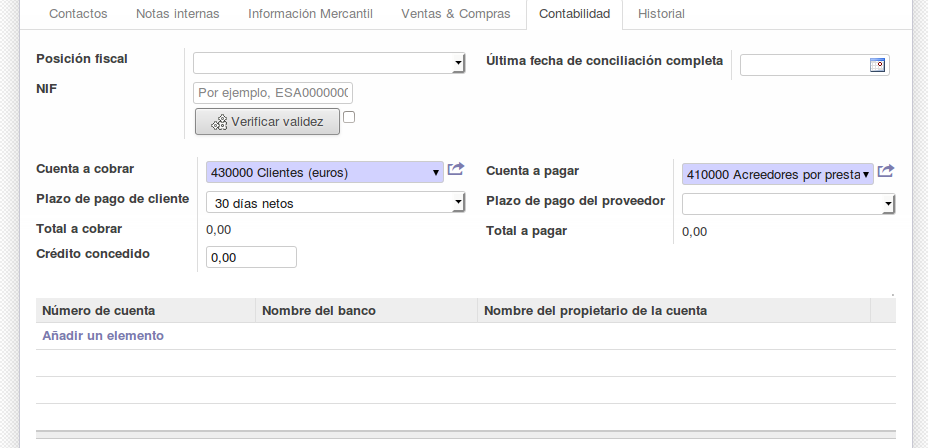
\includegraphics[width=\textwidth]{ventas/img/ven_clicontablidad.png}
\caption{Pestaña de Contabilidad en la ficha del cliente}
\label{ven:clicontabilidad}
\end{figure}



\subsubsection{Pestaña de Historial} 
La pestaña de historial almacena el listado de reclamaciones del cliente. Desde este
mismo punto se pueden añadir nuevas reclamaciones, pero es recomendable añadirlas desde su
sección.


\subsection{Iniciativas}
\label{iniciativas}
Las iniciativas representan clientes y ventas potenciales. Esto quiere decir que una iniciativa no crea una oportunidad de venta real
hasta que se califique si la iniciativa es interesante o no.

Se puede configurar OpenERP para que se creen iniciativas por cada correo recibido en alguna dirección de correo en concreto como info@suempresa.com.


\begin{figure}[H]
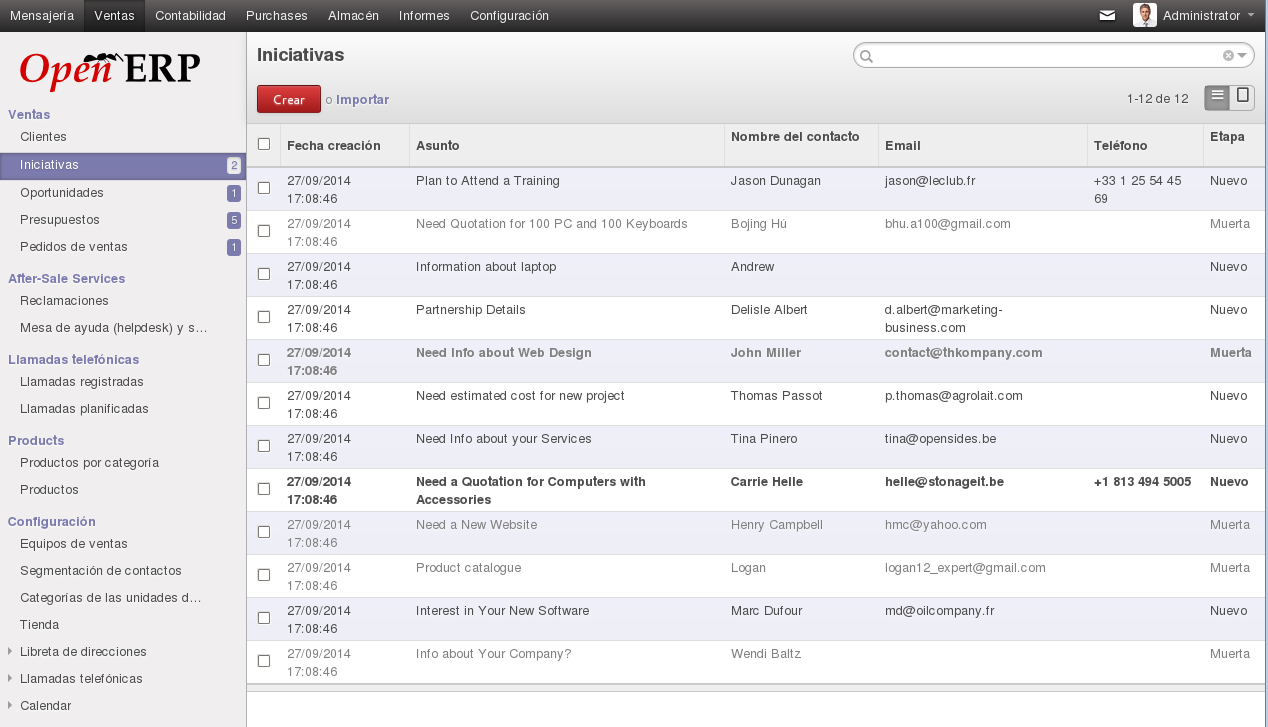
\includegraphics[width=\textwidth]{ventas/img/ven_iniciativas.png}
\caption{Vista de iniciativas}
\label{ven:iniciativas}
\end{figure}

La figura \ref{ven:iniciativas} muestra la vista de las iniciativas al entrar a la misma sección. En la misma se puede apreciar de un
vistazo múltiples iniciativas y sus fechas de creación, nombre del contacto, email y teléfono del mismo. Además, se aprecia el \emph{Asunto} de la 
iniciativa, que corresponde a una breve descripción del asunto a tratar con el cliente. Puede contener una reducida descripción de la posible
venta o algún detalle sobre el contacto.

La \textbf{Etapa} de la iniciativa representa el estado de la misma. Tiene tres posibles estados, aunque uno de ellos no se muestra tal cual (se explica en la descripción del mismo). Estos estados son

\begin{itemize}
  \item \textbf{Nuevo} -- Las iniciativas recien creadas tienen este estado. Se mantienen en este estado hasta que se contacta con el 
                          cliente. Una vez se habla algo con el cliente se pasará la iniciativa a alguno de sus otros estados.
  \item \textbf{Oportunidad} -- Este estado no se mostrará en el listado. Cuando se habla con el cliente relacionado con la iniciativa
                y se puede ver que esta iniciativa, este contacto, puede llevar a alguna venta, se convertirá la iniciativa a oportunidad (mediante el botón \emph{Convertir a oportunidad} que se ve al acceder a la iniciativa).
                En ese momento, se creará una \emph{Oportunidad} en la sección de oportunidades y desaparecerá la iniciativa. Con 
                esto se ha escalado ese contacto a una oportunidad de venta.
  \item  \textbf{Muerta} -- Si tras contactar con el contacto de la iniciativa se aprecia que no existe posibilidad de realizar una venta
               por las razones que sea, se moverá la iniciativa a este estado mediante el botón \emph{Cancelar caso} en la ficha de la 
               iniciativa.
\end{itemize}



\subsubsection{Ficha de iniciativa}

Al hacer click sobre cualquier iniciativa se abrirá la ficha de la misma con toda su información tal como se ve en la figura 
\ref{ven:iniindividual}.

\begin{figure}[H]
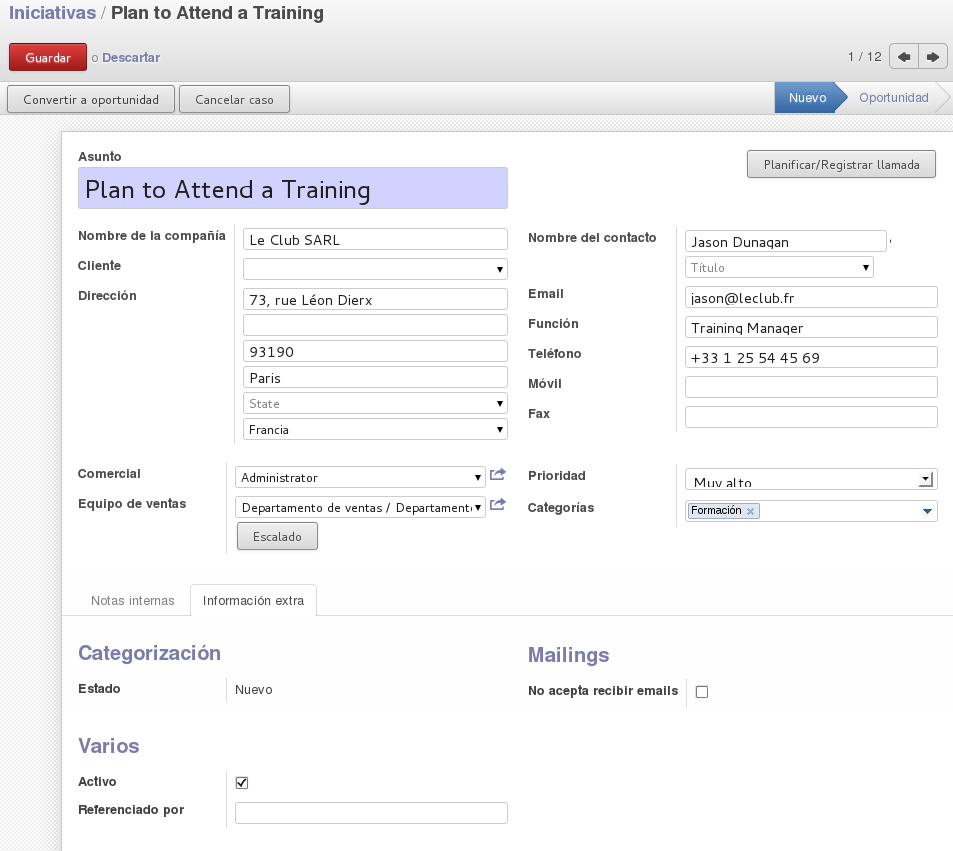
\includegraphics[width=\textwidth]{ventas/img/ven_iniindividual.png}
\caption{Vista de una iniciativa individual}
\label{ven:iniindividual}
\end{figure}

Los datos del contacto se rellenan manualmente. La excepción es si, aunque sea una iniciativa, no es un primer contacto, sino que es un "re-contacto" con un cliente existente, porque el mismo haya mostrado interes o porque se vaya a contactar con él por alguna oferta. En tal caso, eligiendo el cliente adecuado en el campo del mismo nombre, se rellenarán los demás campos de acorde a los datos previamente introducidos del mismo.

A las iniciativas se le pueden asignar distinta \textbf{Prioridad} y varias \textbf{Categorías}, todo ello con caracter de organización interna. Las categorías para ordenar las distintas y las prioridades para agilizar los contactos prioritarios de los que no.

También se puede asignar un \textbf{Comercial} y un \textbf{Equipo de ventas} a las iniciativas. Las iniciativas asignadas a un comercial serán \textbf{vistas sólo por el mismo comercial} al igual que con el equipo de ventas.

Se observa en la parte superior derecha de la ficha de cliente, el botón \emph{Planificar/Registrar llamada}, que permite, como su propio nombre indica, registrar las llamadas hechas/planeadas a ese cliente en relación con esta iniciativa. De las llamadas se habla más concretamente en la sección \ref{llamadas}

Existen dos pestañas en la ficha de iniciativas. La pestaña de \textbf{Notas internas} permite añadir notas de texto a la iniciativa, En el caso de que las iniciativas se creen desde correos electrónicos, esta pestaña contendrá el cuerpo del mensaje recibido.

La pestaña de \textbf{Información extra} contiene la información sobre el \textbf{Estado} de la iniciativa -- vistos anteriormente en el apartado \ref{iniciativas} --, si el cliente \textbf{No acepta recibir emails} y si la iniciativa esta \emph{Activa} y si esta iniciativa está referenciada por alguien.


\subsubsection{Convertir a Oportunidad}
A la hora de convertir a oportunidad la iniciativa, se puede hacer de varias maneras. Al pulsar sobre el botón de conversión a oportunidad, se presentará un dialogo que permitirá elegir distintas opciones -- dialogo representado en la figura \ref{ven:iniaopo}

Por un lado, al convertir a oportunidad puede crearse una nueva oportunidad o fusionarse con una oportunidad ya existente. En el caso de fusionarse con una oportunidad existente, la información de la iniciativa se añadirá a la oportunidad que se indique -- aquella con la que se fusione--.

En el caso de crear una nueva oportunidad, pueden realizarse algunas opciones con los datos del contacto:

\begin{itemize}
  \item \textbf{Crear un nuevo cliente} -- Crea un nuevo cliente con los datos dados. Se muestra la 
        ficha del nuevo cliente para ser completada/confirmada antes de guardar los datos
  \item \textbf{Enlace a un cliente existente} -- Enlaza los datos a un cliente que ya exista para 
        completar los datos que no se tuvieran anteriormente en la ficha del cliente.
  \item \textbf{No enlazar a un cliente} -- Simplemente creará la oportunidad pero no la asociará a 
        ningún cliente.
\end{itemize}

\begin{figure}[H]
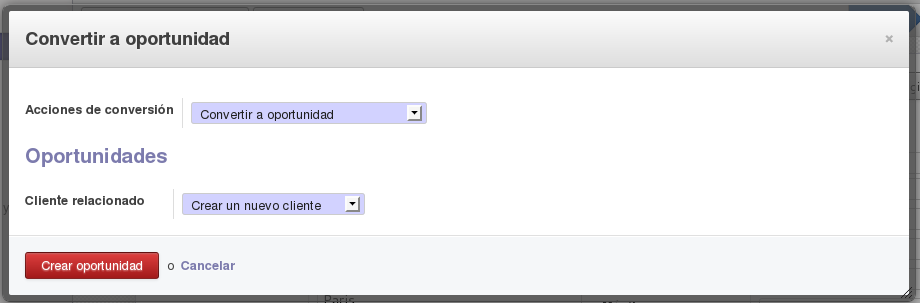
\includegraphics[width=\textwidth]{ventas/img/ven_iniaopo.png}
\caption{Dialogo de conversión de Iniciativa a Oportunidad}
\label{ven:iniaopo}
\end{figure}



\vspace{2cm}
\subsection{Oportunidades}
Mientras que una iniciativa representa un primer contacto con un posible cliente aún por calificar, una oportunidad de venta representa un contrato potencial. Cada oportunidad tiene que ser vigilada por un comercial (o un equipo de ventas) usando su tiempo para calificar la oportunidad, haciendo esto bien a través de una quotation o cancelan la oportunidad.

Las iniciativas son manejadas generalmente por gente diferente, con cierta automatización respondiendo a ciertas entradas o correos. Las oportunidades, por el contrario, son seguidas únicamente por un comercial, debido a que una oportunidad está relacionada con un proceso de negociación con el cliente.

Con las oportunidades, puede administar y realizar el seguimiento del proceso de ventas creando documentos de ventas específicos para cada cliente o cliente potencial. Información como las ganancias esperadas, el estado de la oportunidad, fecha del cierre esperado, historial de comunicación, cuál es la próxima acción y la fecha de la misma y muchas más pueden guardarse en la oportunidad.


\begin{figure}[H]
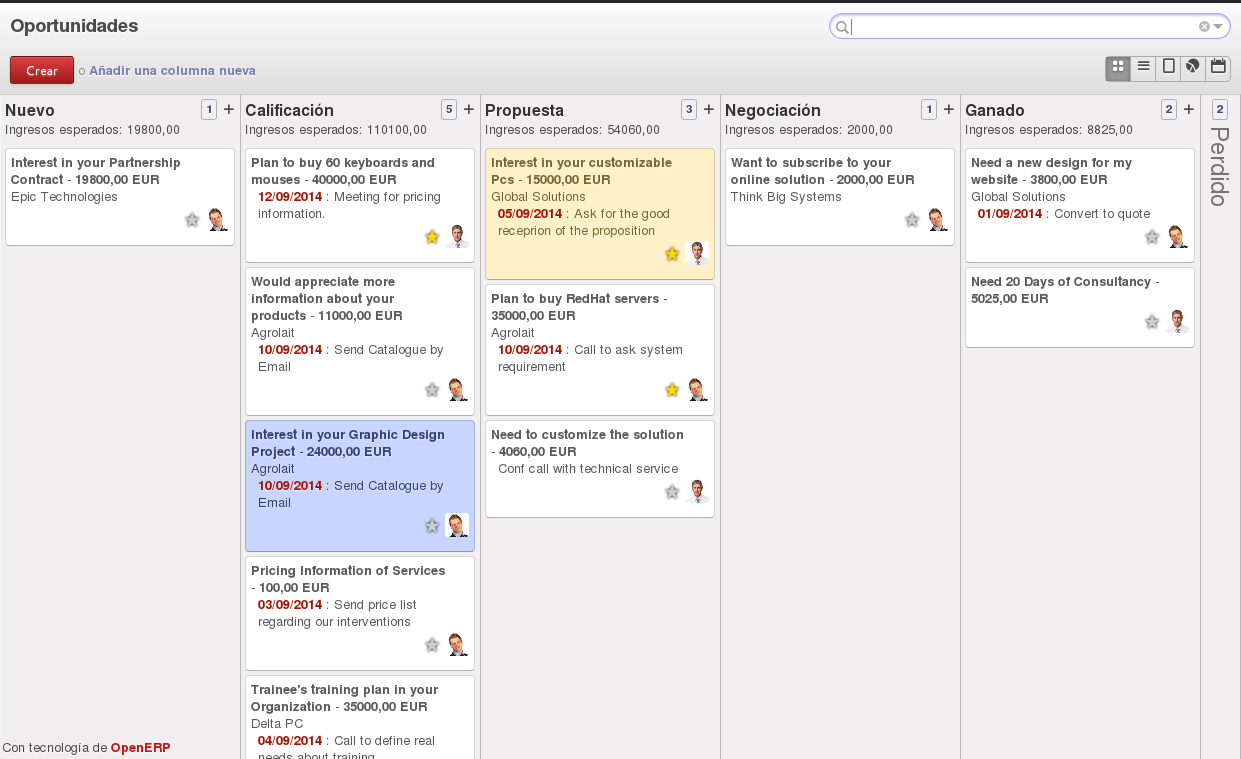
\includegraphics[width=\textwidth]{ventas/img/ven_oportunidades.png}
\caption{Vista Kanban de Oportunidades}
\label{ven:oportunidades}
\end{figure}


\subsubsection{Etapas de las oportunidades}
Al entrar en las oportunidades, se podrá ver una distribución como la mostrada en la figura \ref{ven:oportunidades}. En esta vista tipo 
Kanban, cada columna representa un estado para la oportunidad. Estos estados mostrados por defecto son los \emph{sugeridos} por OpenERP. No obstante, son modificables tanto en número como en nombre, de manera que se adapten más eficientemente al proceso seguido por la empresa.

Estos estados sugeridos por OpenERP pueden entenderse de la siguiente manera:

\begin{description}
   \item[Nueva] -- Estado inicial de las oportunidades. Aquí se sugiere la segmentación de estas oportunidades geográficamente. En este
                punto se hace esa clasificación y se asigna a un comercial. De ahí se pasaría a su siguiente estado.
   \item[Calificación] -- En este punto se trata de que el encargado de la oportunidad atraiga la atenció ndel cliente, determinando 
                las necesidades del mismo. Se trata de encontrar esa necesidad del cliente de comprar un producto o servicio. 
                Cuando esta necesidad está confirmada se da un paso más y se pasa al siguiente estado.
   \item[Propuesta] -- En este momento, el encargado de la oportunidad se encuentra discutiendo con el cliente cuáles son sus necesidades,
                recomendando soluciones específicas para mostrar al cliente. Se espera de esta fase que aparezca una propuesta de compra
                o la necesidad de ver una demo\ldots etc. Se trata de acabar viendo que el cliente tiene interes en la compra.
   \item[Negociación] -- Cuando el cliente muestra interés en la compra se comienza esta fase. Se busca afinar cuál será la compra, las
                condiciones de la misma y el contrato. En esta fase se incluye el envío del contrato para su firma -- o su firma      
                directamente.
   \item[Ganado/Perdido] -- Según la negociación haya llegado a buen o mal puerto, la oportunidad pasará a su estado de ganada
                en el caso de que finalmente el cliente firme por la compra del producto/servicio. Será perdida si finalmente el cliente
                rechaza cualquier tipo de compra o adquisición.
\end{description}

\vspace{2cm}
\subsubsection{Ficha de oportunidad}

\begin{figure}[H]
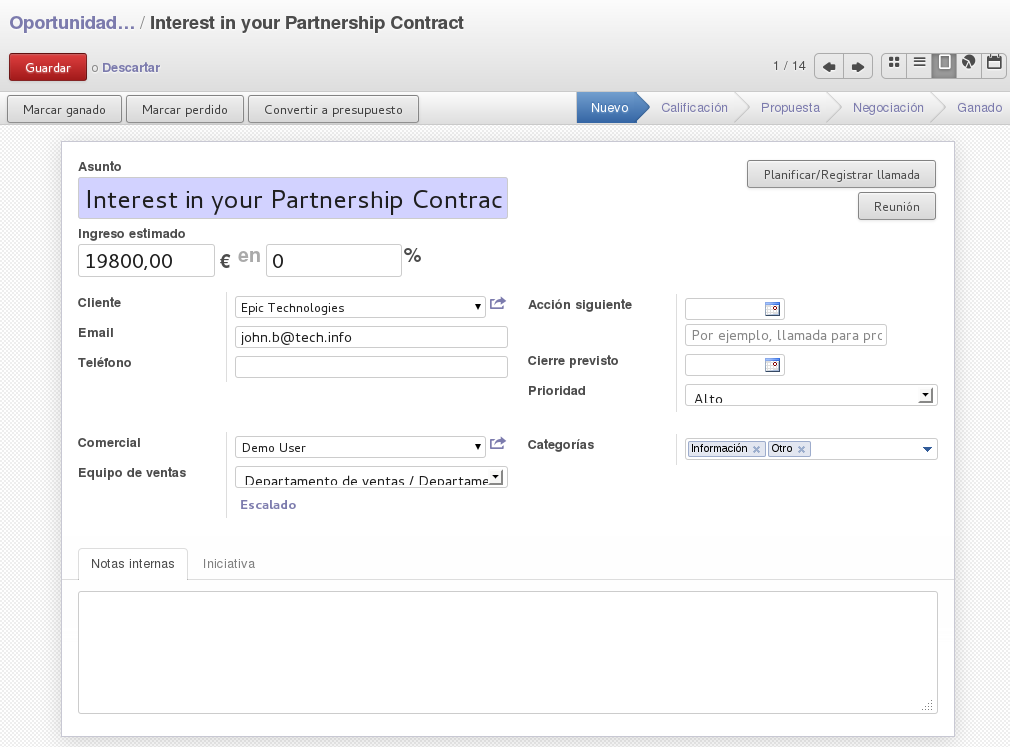
\includegraphics[width=\textwidth]{ventas/img/ven_opoindividual.png}
\caption{Vista de una oportunidad individual}
\label{ven:opoindividual}
\end{figure}

La ficha individual de una \emph{Oportunidad} se puede observar en la figura \ref{ven:opoindividual}. En la parte superior izquierda se 
aprecian unos botones que permiten pasar la oportunidad al estado de \emph{Ganado} o \emph{Perdida} independientemente del estado en el que se encuentre. También se ve un tercer botón que permite pasar la oportunidad directamente a un \textbf{presupuesto}, que marcará, además, la oportunidad como ganada. La información sobre los presupuestos se amplía en el capítulo \ref{presupuestos}.

Al mismo nivel, a la derecha, se pueden observar todos \textbf{los posibles estados} de la Oportunidad. El estado actual se encuentra
marcado en azul. Pulsando sobre los distintos estados podemos variar el estado actual de la oportunidad seleccionada, es la manera 
más sencilla y rápida de cambiar de estado.

Un poco más abajo se pueden observar los botones de \textbf{Planificar/Registrar llamada} y \textbf{Reunión}. El primero sirve para la creación/revisión de las llamadas relacionadas con esta oportunidad, mientras que el de reunión permite crear un nuevo evento en el calendario. Mostrará en primer lugar el calendario y al seleccionar el día rellenará los datos relacionados con el cliente de la reunión
siendo el creador de la reunión el responsable de rellenar el resto de información y de completar quienes serán los asistentes.

El \textbf{Asunto} es una breve descripción de la oportunidad, que será el texto por el que se le identificará cuando se observe la lista de oportunidades. El \textbf{Ingreso estimado} es una aproximación a la cantidad de dinero que se podría obtener con esta oportunidad, y el \textbf{porcentaje} que se situa a su lado es la probabilidad de que la oportunidad acabe en buen puerto. Este porcentaje es hasta cierto punto subjetivo y lo puede rellenar el mismo usuario. Estos datos pueden ser importantes para un análisis de oportunidades y para poder
analizar a posteriori posibles fallos y localizar posibles fallos en el proceso de venta.

Del resto de datos de la ficha cabe recalcar la importancia de los campos \textbf{Acción siguiente}, que permite indicar la fecha en la que
se realizará alguna acción en relación a esta oportunidad y una descripción de este paso (como por ejemplo, la fecha de la próxima llamada y usando como descripción "Llamar con el descuento preparado"). También el campo \textbf{cierre previsto} es importante para calculos
empresariales y hacer un seguimiento más detallado de la venta. Por supuesto que este campo es modificable una vez llegada la fecha,
no se puede estimar el cierre con un 100\% de seguridad, pero con esta información se consigue agilizar el análisis de los movimientos comerciales por parte del encargado de la supervisión de los mismos.

El resto de campos son como los vistos hasta ahora, \textbf{Comercial} y \textbf{Equipo de ventas} refieren al encargado (y su equipo) de
la oportunidad. La \textbf{prioridad} permite ordenar por importancia las oportunidades, y \textbf{Categorías} permite tener organizadas
todas las oportunidades en distintas áreas para supervisarlas independientemente.

La pestaña de \textbf{Notas internas} es, al igual que las vistas anteriormente, un área para guardar información en formato de texto 
plano relacionada con la Oportunidad y la pestaña \textbf{Iniciativa} guarda los datos de contacto y otros introducidos en la Iniciativa
que dió lugar a la oportunidad visualizada. Hay más información sobre los campos de esta pestaña en el capítulo \ref{iniciativas}.


\subsection{Presupuestos}
\label{presupuestos}
Parece innecesario describir un presupuesto a estas alturas. Podemos entenderlo en este punto como una oportunidad que ha sido ganada
y se ha transformado en una venta concreta por confirmar.

Los presupuestos contienen los productos a vender, los datos del cliente y las condiciones de las ventas. En su visión de listado se observan los datos básicos (figura \ref{ven:prelista})
\begin{figure}[H]
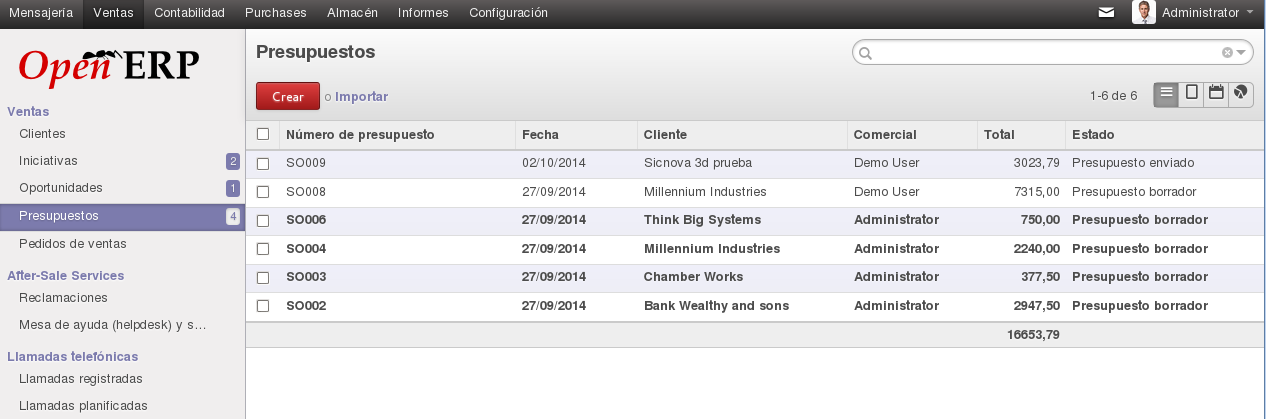
\includegraphics[width=\textwidth]{ventas/img/ven_prelista.png}
\caption{Listado de presupuestos}
\label{ven:prelista}
\end{figure}

La vista del listado es más informativa a nivel general, se puede apreciar en la misma el \textbf{nº del presupuesto}, \textbf{su fecha}, 
\textbf{cliente}, \textbf{comercial} al cargo del presupuesto y el \textbf{total}, que hace referencia al precio total de la venta. Además se aprecia el campo \textbf{estado} que indica en que punto está el presupuesto, sus posibles estados son:

\begin{description}
  \item[Presupuesto borrador] -- Es un presupuesto no confirmado, pendiente de darle el visto bueno y ser enviado al cliente.
  \item[Presupuesto enviado] -- Estado que se alcanza tras el envío del presupuesto al cliente.
  \item[Excepción] -- Este estado se asigna cuando ocurre alguna excepción con el almacén (relacionado con los productos indicados en el
                      presupuesto) o en la factura (la que esté en relación a este presupuesto/orden de venta)
\end{description}
\vspace{1cm}


\subsubsection{Ficha de presupuesto individual}
\begin{figure}[H]
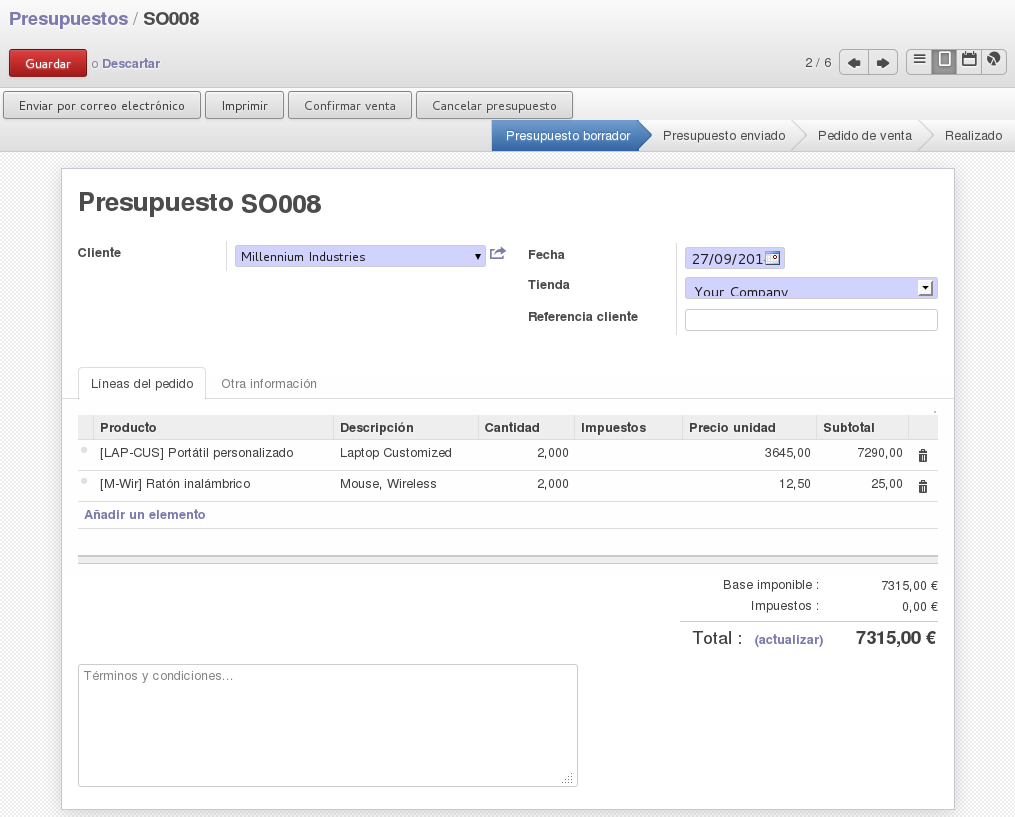
\includegraphics[width=\textwidth]{ventas/img/ven_preindividual.png}
\caption{Ficha individual de presupuesto}
\label{ven:preindividual}
\end{figure}

La figura anterior(\ref{ven:preindividual}) muestra la ficha individual de un presupuesto. Desde la ficha se indica el cliente -- lo que rellenará automáticamente la dirección que se puede apreciar -- la \textbf{fecha de la venta}, la \textbf{tienda} -- habitualmente sólo 
será una y no será necesario cambiarla -- y se puede añadir una \textbf{referencia cliente} a mano.

Las \textbf{líneas de pedido} representan los productos que se venden y se facturan en el presupuesto -- y en la factura final --. Pueden añadirse tantas como sean necesarias. Al seleccionar un nuevo producto, el resto de los elementos de la línea (Descripción, Impuestos, Precio Unidad\ldots) se rellenarán automáticamente con los datos del producto (que se pueden ver en la sección \ref{productos}), pudiendo añadir, eliminar o modificar estas propiedades también aquí si fuera necesario -- se pueden añadir impuestos, modificar el precio \ldots.

Hay que recordar que \textbf{cuando se modifiquen líneas de productos} de un presupuesto, ya seá modificando el número de productos o
variando el impuesto, utilizar la acción \textbf{actualizar} que se puede ver en la línea del total del presupuesto, asegurandose de que se refresca la cantidad y se adapta a los nuevos datos.

Los botones que se observan en la parte superior izquierda de la ficha permiten \textbf{Enviar por correo el presupuesto} directamente al
cliente (o las direcciones que sean necesarias), \textbf{Imprimir} el presupuesto y \textbf{Confirmar la venta} o \textbf{Cancelar el presupuesto}. La confirmación de la venta hará que el presupuesto desaparezca de esta sección y que aparezca en el apartado de \emph{Pedidos de ventas}, el cual se explica en la sección \ref{pedidosventas}

\begin{figure}[H]
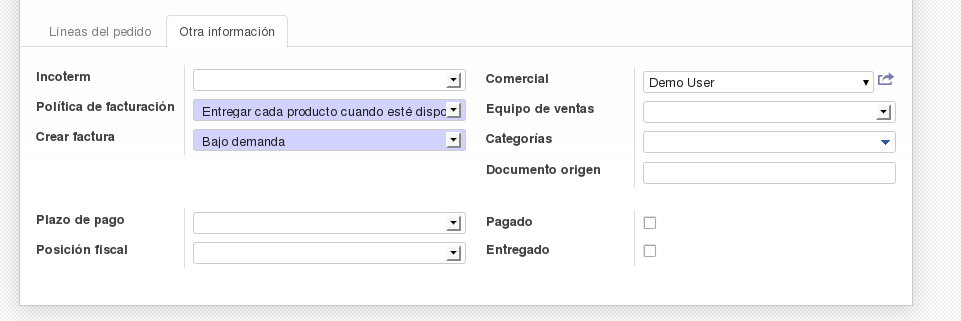
\includegraphics[width=\textwidth]{ventas/img/ven_preindotra.png}
\caption{Pestaña \emph{Otra información} de presupuesto}
\label{ven:preindotra}
\end{figure}

La otra pestaña que se encuentra junto a la de \emph{Líneas de pedido} es \textbf{Otra información}. En ésta (visible en la figura 
\ref{ven:preindotra}). La información obligatoria en este caso es:

\begin{itemize}
  \item \textbf{Política de facturación} -- Permite elegir la política de entrega y facturación de los productos.
  \begin{itemize}
    \item[$\star$] \textbf{Entregar cada producto cuando esté disponible} -- Utilizado para ir sirviendo los productos a medida que se encuentren 
          disponibles en el stock.
    \item[$\star$] \textbf{Entregar todos los productos a la vez} -- Espera a que todos los productos se encuentren disponibles en stock para realizar la
          facturación y envío.
  \end{itemize}

  \item \textbf{Crear factura} -- Indica como se va a realizar la facturación.
    \begin{itemize}
      \item[$\star$] \textbf{Bajo demanda} -- Se crea la factura desde la orden de venta a petición del comercial
      \item[$\star$] \textbf{Sobre la orden de entrega} -- Crea la factura cuando se completa el envío y la entrega de productos al cliente.
      \item[$\star$] \textbf{Antes de la entrega} -- Se crea la factura cuando se confirma el borrador, y no se realiza el envío y entrega de productos hasta
           que la factura esté pagada.
    \end{itemize}
\end{itemize}

Se puede añadir además un \textbf{Plazo de pago} y una \textbf{posición fiscal}, utilizando esta última automáticamente en el área de 
contabilidad, creando los asientos de acuerdo a este elemento también.

El \textbf{Documento de origen} hace referencia al documento original del que deviene este presupuesto, aunque no se utiliza habitualmente puede adaptarse a las necesidad de la empresa.


\subsection{Pedidos de ventas}
\label{pedidosventas}

Los pedidos de ventas son, a nivel de la aplicación, idénticos a los presupuestos salvo que hacen referencia a pedidos de clientes que hay que facturar y enviar, esto es, ventas realizadas. Además, se encuentran en secciones separadas para no ser confundidos con presupuestos, y sus estados son distintos.

\begin{figure}[H]
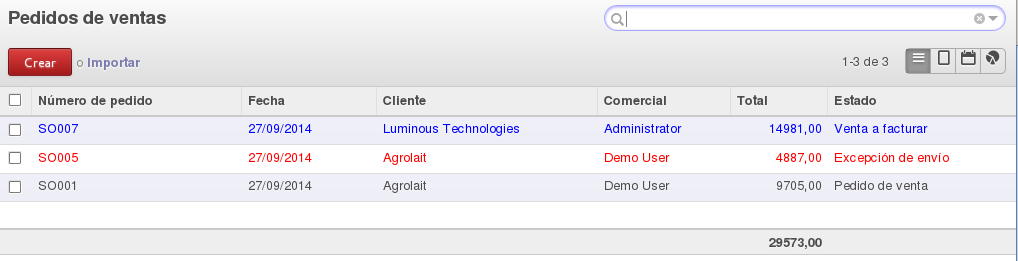
\includegraphics[width=\textwidth]{ventas/img/ven_pedlistado.png}
\caption{Listado de los pedidos de venta}
\label{ven:pedlistado}
\end{figure}

La diferencia básica estriba en la visión individual del pedido de venta tal como se ve en la figura \ref{ven:pedindividual}. En la botonera de la parte superior izquierda se aprecian otros botones con otro texto. En el caso más interesante -- que es cuando la creación de la factura se crea antes del envío -- en el pedido confirmado aparecerá el botón \textbf{Ver factura}. Este botón permite al comercial al cargo del pedido de venta ver la factura del mismo y el estado en el que se encuentra. Aunque el comercial no tenga acceso a la zona de contabilidad, si puede hacer un seguimiento de los documentos relacionados con sus ventas, sólo en modo lectura, es decir, no puede validad ni manipular la factura de ninguna manera, tan solo verla y los datos relacionados con ella.

\begin{figure}[H]
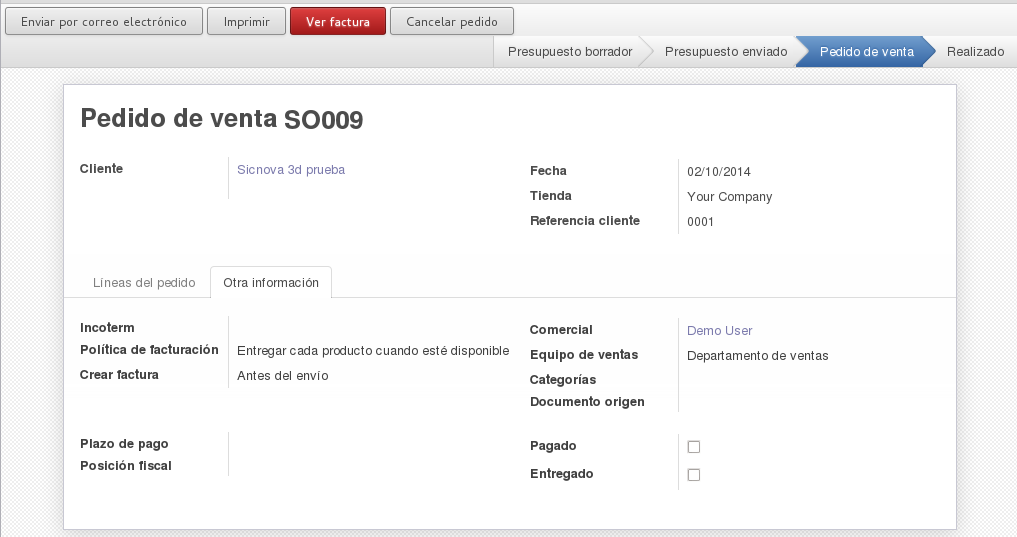
\includegraphics[width=\textwidth]{ventas/img/ven_pedindividual.png}
\caption{Pedido de venta individual}
\label{ven:pedindividual}
\end{figure}

Cuando la factura se registre como pagada en la sección de contabilidad, se creará una orden de envío en el almacén, y aparecerá un nuevo
botón en el pedido de venta, denominado \textbf{Ver orden de entrega}. Este botón, al igual que el de \emph{Ver factura}, permite echar un
vistazo a la orden de envío del almacén, de manera que el comercial puede hacer un seguimiento del envío de su venta. De igual modo que la
factura, sólo puede visualizar la información, no manipularla directamente, ya que de eso se encarga la persona responsable del almacén.




\section{Servicio Post-venta}

Los servicios post-venta se dividen en reclamaciones -- incidencias y problemas que ha habido en una venta/producto -- y peticiones de ayuda (Helpdesk) -- dudas y cuestiones varias por parte de un cliente.

La diferencia básica se encuentra en que las reclamaciones se crean para aceptarlas y solucionarlas o para rechazarlas. Por ejemplo, la
venta de una impresora a la que le faltan las llaves de la puerta sería una reclamación. Esta se acepta, se envían unas llaves y se cierra
la reclamación como resuelta.

Si un cliente tiene una duda sobre un uso concreto poco documentado, éste puede llamar para preguntar y se crearía una entrada en la
sección \emph{Helpdesk}. A partir de aquí el estado de esta pregunta se puede abrir y desarrollar a lo largo del tiempo hasta conseguir
explicarle al cliente esa funcionalidad, crearle un manual\ldots etc. En ese punto se marcaría como resulta.

La diferencia básica está en que las incidencias ocurren y deben ser resueltas en un proceso documentado. Las peticiones de ayuda para helpdesk pueden conllevar una conversación con el cliente y suelen ser preguntas y acciones concretas que no requieren de un desarrollo -- o al menos de un desarrollo extenso -- de su solución. Si se requieriera, estaríamos hablando de una reclamación, una incidencia o fallo
que requiere trabajarla para evitar que se repita.




\subsection{Reclamaciones}

\begin{figure}[H]
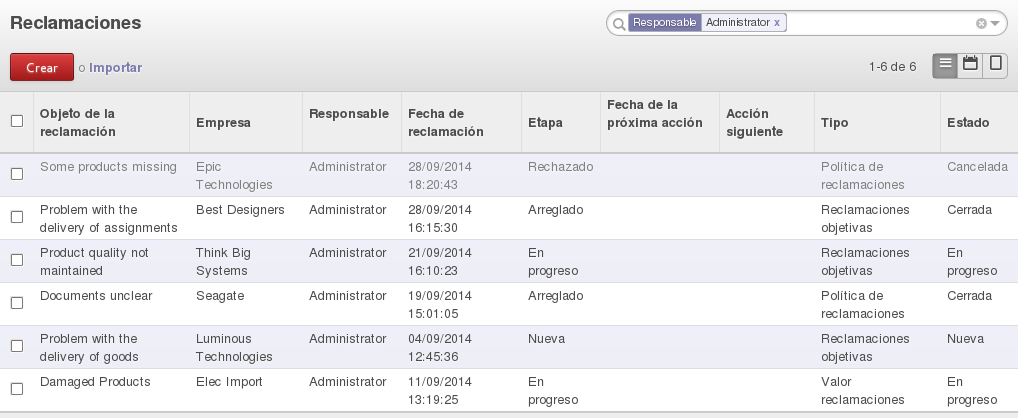
\includegraphics[width=\textwidth]{ventas/img/ven_reclista.png}
\caption{Listado de incidencias}
\label{ven:reclista}
\end{figure}

La figura \ref{ven:reclista} muestra el listado de incidencias, la visión general que se da al entrar en la sección de las mismas. De un
vistazo se pueden ver la información principal. \textbf{Objeto de la reclamación} contendrá un pequeño resumen de la incidencia. En 
\textbf{Empresa} se refleja el cliente que ha generado la incidencia, también se indica el \textbf{Responsable} y \textbf{Fecha de creación}.
La \textbf{Etapa} en la que se encuentra la incidencia. Estas etapas pueden ser:

\begin{description}
  \item[Nueva] -- Cuando se crea la reclamación, este será la etapa que se le asigna por defecto.
  \item[En progreso] -- Si se inician unos trámites que requieran de varios pasos o alargar en el tiempo la incidencia, se le deberá asignar
                     esta etapa. Para poder usar esta etapa habrá que hacer click sobre su nombre en el listado de etapas que figura en la 
                     ficha individual de reclamación, en la parte superior derecha de la misma.
  \item[Arreglado] -- Esta etapa se alcanza cuando se resuelve la reclamación.
  \item[Rechazado] -- Si la reclamación finalmente no resulta como tal, se rechaza y quedará constancia de que esa reclamación realizada
                      por el cliente no es responsabilidad de la empresa.
\end{description} 

La \textbf{Fecha de la próxima acción} y \textbf{Acción siguiente} dan, en este modo de presentar las reclamaciones, una vista rápida del siguiente paso a dar -- el qué y el cuándo -- para resolver la reclamación. El campo \textbf{Estado} representa lo mismo que \textbf{Etapa} en este caso.

\subsubsection{Ficha de reclamación}

\begin{figure}[H]
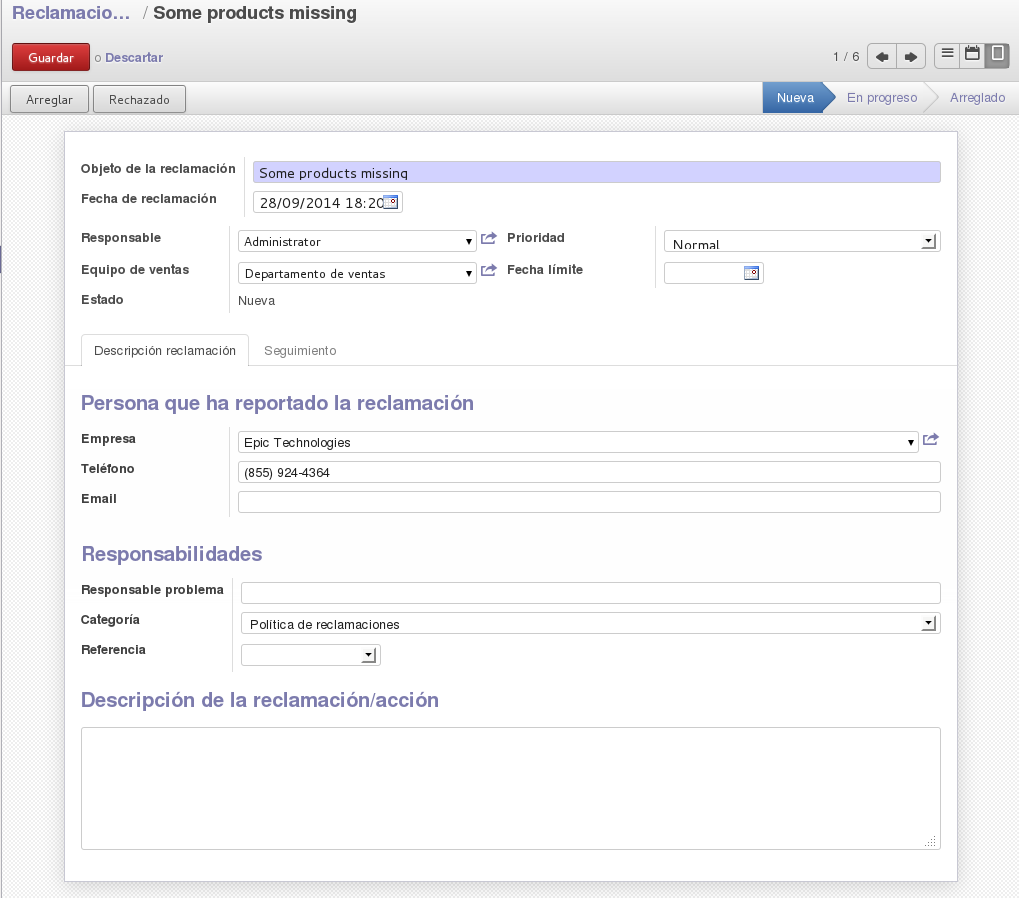
\includegraphics[width=\textwidth]{ventas/img/ven_recindividual.png}
\caption{Ficha de reclamación}
\label{ven:recindividual}
\end{figure}

En la ficha de la reclamación se rellenarán los datos sobre la misma (como se ve en la figura \ref{ven:recindividual}) siendo importante siempre
el utilizar una fecha límite para evitar retrasos en la resolución de problemas. Esta fecha límite debería ser una norma según la empresa que lleve las reclamaciones para evitar problemas que queden sin resolver.

La otra pestaña disponible (\textbf{Seguimiento}) se utiliza para temporizar y hacer el seguimiento detallado del problema expuesto en la
reclamación (figura \ref{ven:recseguimiento})

\begin{figure}[H]
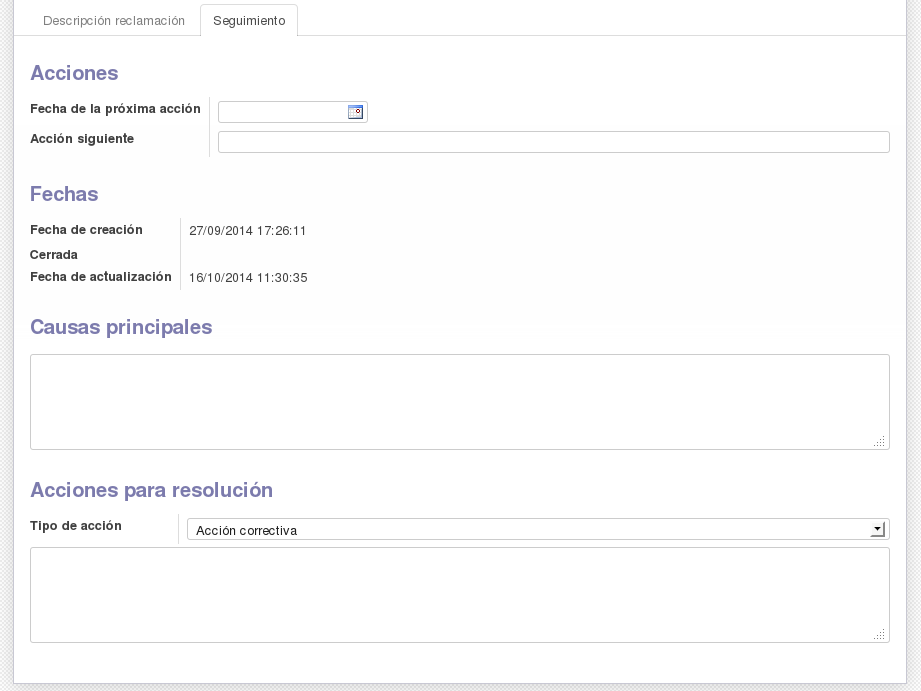
\includegraphics[width=\textwidth]{ventas/img/ven_recseguimiento.png}
\caption{Pestaña de seguimiento en la ficha de reclamación}
\label{ven:recseguimiento}
\end{figure}

Es importante rellenar siempre la \textbf{Acción siguiente} y su \textbf{Fecha de próxima acción} para una gestión eficiente de las 
reclamaciones. El rellenar también las \textbf{Causas principales} y \textbf{Acciones para resolución} ahorrará tiempo en el futuro, tanto
al encargado de resolver la reclamación como a cualquier otro que requiera intervenir en la misma, además de ofrecer información sobre
los problemas que se van encontrando al supervisor del área.

\subsection{Helpdesk}
A continuación, en la figura \ref{ven:hellistado} se muestra la vista en forma de lista de las peticiones de ayuda.

\begin{figure}[H]
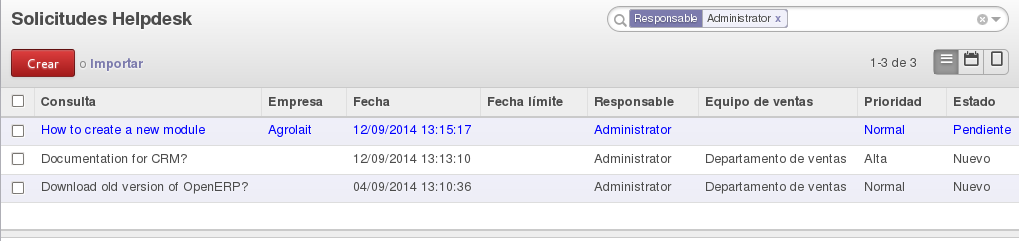
\includegraphics[width=\textwidth]{ventas/img/ven_hellistado.png}
\caption{Listado de peticiones de ayuda (helpdesk)}
\label{ven:hellistado}
\end{figure}

De igual modo que en las reclamaciones, aquí se ofrece una visión generalizada de las peticiones existentes y una descripción breve
de las mismas. Se observa una distribución distinta de los campos a pesar de que la información que muestran es la misma. La \textbf{Fecha límite} es igual de importante que cuando se mencionó en las reclamaciones.

\subsubsection{Ficha de Helpdesk}

\begin{figure}[H]
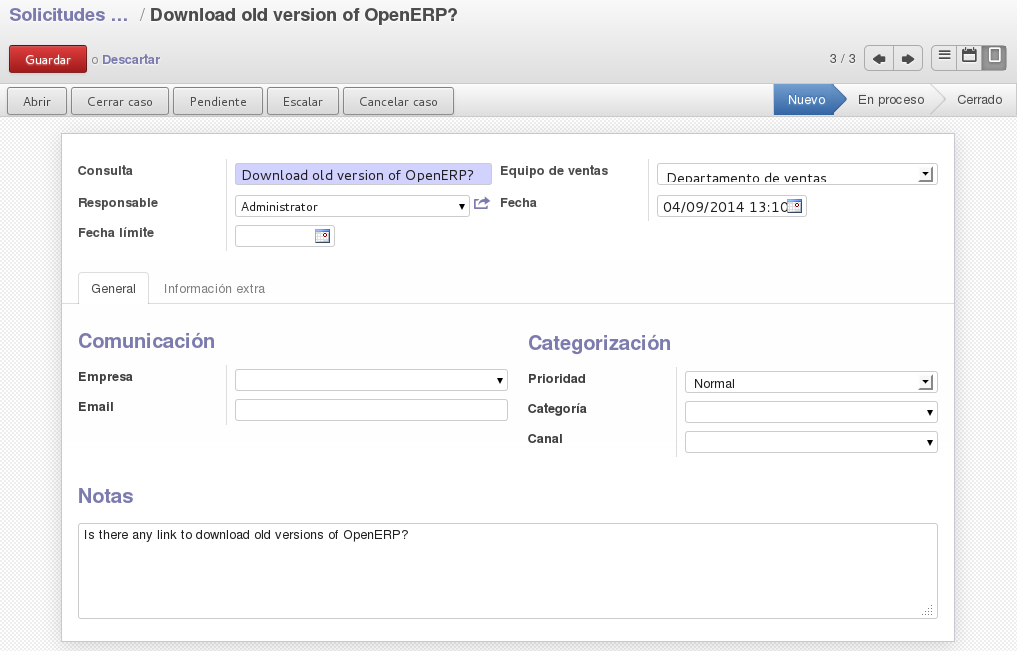
\includegraphics[width=\textwidth]{ventas/img/ven_helindividual.png}
\caption{Ficha individual de Helpdesk}
\label{ven:helindividual}
\end{figure}

La ficha de Helpdesk individual mostrada en la figura superior (\ref{ven:helindividual}) muestra los detalles de la petición de ayuda.
La sección \textbf{Comunicación} se utiliza para introducir los datos de la empresa/cliente que genera la petición de ayuda. En \textbf{Categorización} se clasifica la petición en categorías y prioridades. También se le puede asignar un \textbf{Canal}, que hace referencia
al canal por el cuál ha llegado la petición -- algunos ejemplos son: por email, teléfono, a través de web\ldots --. Y por supuesto en el apartado de \textbf{Notas} se detalla la petición de ayuda con más detalle.

En la pestaña de \textbf{Información extra} (figura \ref{ven:helextra}) pueden añadirse \textbf{Referencias} como la empresa que generó la consulta, una factura relacionada, eventos, números de serie\ldots Al igual que añadir si va a llevar algún coste resolver esta duda para poder facturarlo a posteriori.

\begin{figure}[H]
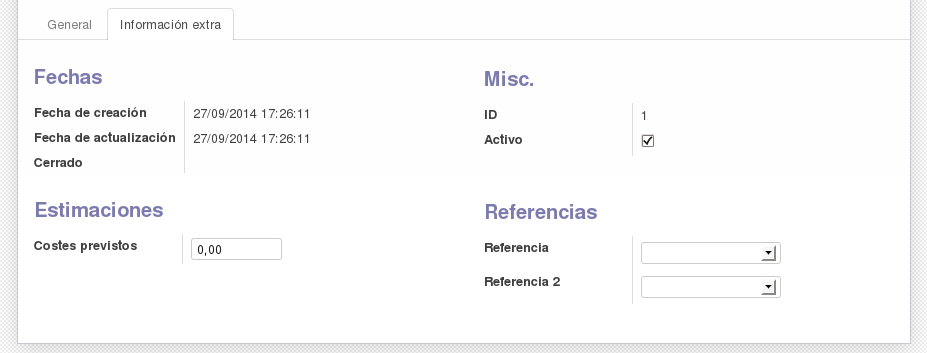
\includegraphics[width=\textwidth]{ventas/img/ven_helextra.png}
\caption{Pestaña \emph{Información extra} de Helpdesk}
\label{ven:helextra}
\end{figure}




\section{LLamadas telefónicas}
\label{llamadas}

Con las llamadas se puede tener un control informativo sobre los contactos hechos a través de teléfono con clientes y/o clientes potenciales. También para organizar comercialmente las llamadas, pudiendo planificar llamadas, extraer conclusiones y generar reuniones, todo directamente desde esta sección.

Hay dos tipos de llamadas en el software. Unas son las \textbf{llamadas registradas} que son aquellas que se registran como ya hechas, a cliente contactado, y las \textbf{llamadas planificadas}

\subsection{Llamadas registradas}
Las llamadas realizadas las conforman el registro de llamadas ya hechas a clientes. Es una sección sencilla, la única visión es en forma
de lista como se ve en la figura \ref{ven:llarealizadas}.

\begin{figure}[H]
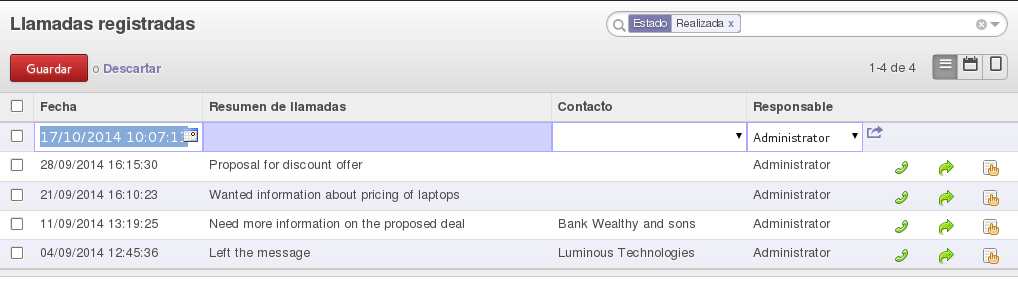
\includegraphics[width=\textwidth]{ventas/img/ven_llarealizadas.png}
\caption{Listado de llamadas realizadas}
\label{ven:llarealizadas}
\end{figure}

Los campos resultan bastante intuitivos, la \textbf{fecha}, el \textbf{Resumen de llamadas}, \textbf{Contacto} y \textbf{Responsable} se 
completaran con los datos descritos por el mismo campo. En el caso del \emph{Contacto} se puede realizar la busqueda del cliente a través
del desplegable, al igual que del \textbf{Responsable}.

En la parte derecha de cada llamada registrada hay tres iconos que permiten distintas acciones a partir de la información de la llamadas, son los siguientes:

\begin{itemize}
  \item \textbf{Teléfono} -- Con este botón se puede generar una nueva llamada registrada o planificar una nueva llamada. Al pulsarlo se 
                           abrirá una ventana con los datos rellenados -- y modificables por el que esté creando esta nueva llamada -- en 
                           un diálogo que se puede ver en la figura \ref{ven:llacrear}
  \item \textbf{Flecha verde} -- Crea una nueva reunión a partir de la llamada. Al pulsar, se abrirá la visión del calendario, donde se 
                           podrá pinchar en cualquier día para crear ahí la nueva reunión. Al pulsar sobre el día se abrirá un dialogo 
                           complementario para introducir todos los datos de la reunión.
  \item \textbf{Icono de la mano} -- Convierte la llamada en una oportunidad. Crea la oportunidad y automáticamente introduce los datos
                           del contacto -- los que hubiera en la llamada -- en la oportunidad. El resto de datos puede introducirlos o
                           modificarlos el usuario.
\end{itemize}

\begin{figure}[H]
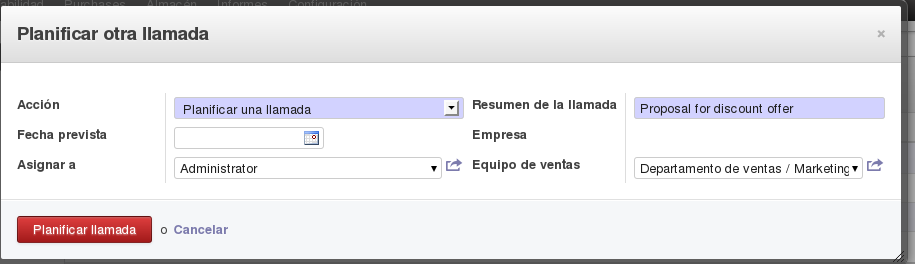
\includegraphics[width=\textwidth]{ventas/img/ven_llacrear.png}
\caption{Diálogo para crear una nueva llamada a partir de una registrada}
\label{ven:llacrear}
\end{figure}




\subsection{Llamadas planificadas}

Estas llamadas son las que están por realizar. La vista principal al entrar en esta sección es en forma de lista (figura \ref{ven:llaplanificadas}). Los campos que coinciden en nombre con los descritos en las llamadas realizadas cumplen las mismas funciones,
\textbf{Fecha}, \textbf{Resumen de llamada}, \textbf{contacto}, \textbf{teléfono} y \textbf{responsable} no necesitan una descripción más allá de su propio nombre.

En el caso del \textbf{Estado} sólo podrá ser \emph{Confirmado}, refiriendos a que la llamada está creada y confirmada, y \emph{Realizada}, una vez hecha. En ese punto, la llamada se moverá automáticamente al listado de llamadas realizadas. Si se \emph{cancela} una llamada puede alcanzar un estado del mismo nombre. La llamada cancelada se verá en gris, no desaparece del todo para, en caso necesario, volver a activarla.

\begin{figure}[H]
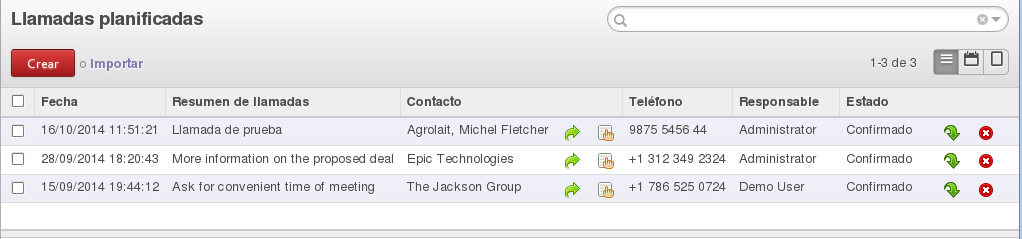
\includegraphics[width=\textwidth]{ventas/img/ven_llaplanificadas.png}
\caption{Diálogo para crear una nueva llamada a partir de una registrada}
\label{ven:llaplanificadas}
\end{figure}

Al igual en las llamadas realizadas, aquí se aprecian algunos iconos que dotan de acciones extra a las llamadas. En el area central se
pueden apreciar dos iconos, identicos en aspecto y funcionalidad a los vistos en las llamadas registradas, en este caso son dos en lugar 
de tres y son:

\begin{itemize}
  \item \textbf{Flecha verde} -- Crea una nueva reunión a partir de la llamada. Al pulsar, se abrirá la visión del calendario, donde se 
                           podrá pinchar en cualquier día para crear ahí la nueva reunión. Al pulsar sobre el día se abrirá un dialogo 
                           complementario para introducir todos los datos de la reunión.
  \item \textbf{Icono de la mano} -- Convierte la llamada en una oportunidad. Crea la oportunidad y automáticamente introduce los datos
                           del contacto -- los que hubiera en la llamada -- en la oportunidad. El resto de datos puede introducirlos o
                           modificarlos el usuario.
\end{itemize}

Además de estos, hay dos iconos más en la parte derecha de cada elemento de la lista de llamadas planificadas:

\begin{itemize}
  \item \textbf{Flecha verde hacia abajo} -- Indica que la llamada ha sido realizada. Convierte la llamada planificada en realizada y 
                           la pasa automáticamente al listado de llamadas realizadas.
  \item \textbf{Circulo rojo con X} -- Cancela la llamada, pasandola a su estado de \emph{Cancelada}.
  \item \textbf{Figuras geométricas con una flecha} -- Este icono sólo aparece cuando la llamada está en el estado de \emph{Cancelada}.
                           su función es pasar la llamada de nuevo a \emph{para hacer}, reactivandola y devolviendola al estado de 
                           confirmada. Cuando aparece este icono -- al estar en el estado de cancelada -- los demás iconos, a excepción 
                           del de crear una oportunidad a través de la llamda, desaparecen.
\end{itemize}


\subsubsection{Ficha de llamada planificada}

\begin{figure}[H]
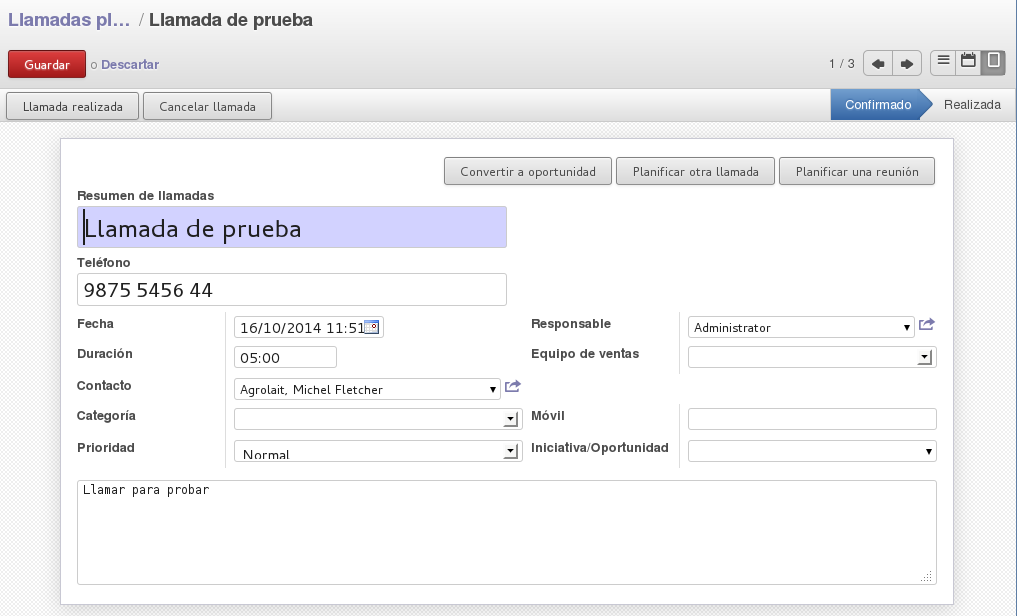
\includegraphics[width=\textwidth]{ventas/img/ven_llaindividual.png}
\caption{Ficha de una llamada planificada}
\label{ven:llaindividual}
\end{figure}

En la imagen superior (figura \ref{ven:llaindividual}) se observa la ficha de una llamada planificada. La zona superior, habilitada con
múltiples botones, realizan las funciones que se han visto en los iconos que aparecen en las llamadas cuando se ve en forma de listado.

Los campos son los mismos que los vistos hasta ahora. Con \textbf{Categoría} y \textbf{Prioridad} se puede realizar la clasificación 
vista en otras secciones para organizar y gestionar correctamente las llamadas. El \textbf{Responsable} y \textbf{Equipo de ventas} clasifican las llamadas de manera que cada usuario de esta sección pueda ver sólo las llamadas de las que es responsable y, a la vez, dar
una estructura de permisos para generar supervisores más o menos generales de las llamadas.

El campo \textbf{Iniciativa/Oportunidad} sirve para relacionar la llamada que se está creando con una iniciativa u oportunidad ya existente. Asociandolas de esta manera se podrá, después, acceder desde la iniciativa u oportunidad a esta y las demás llamadas relacionadas con ella, pudiendo hacer un seguimiento de como se ha tratado esa inciativa/oportunidad por parte del responsable.

%\section{Productos}


%
% Este archivo es parte de un documento sobre OpenERP/Odoo creado
% y distribuido bajo licencia GNU Free Documen License v1.3.
%
% Para obtener la fuente e información más detallada, visite
% https://github.com/Gabriel-fm/oerp-manual
%
% Copyright (c) 2014 - Gabriel Franco
%

\chapter{Módulo de Contabilidad}

\section{Conceptos previos de Contabilidad}

En este módulo se utilizan lo que se conocen como \textbf{diarios}.

Los \textbf{diarios} no son más que una forma más de agrupar los datos. Las facturas, por ejemplo, pueden guardarse en distintos \emph{diarios}. Esto, al final, no influye en ningún elemento de la factura ni en la gestión de las mismas, siguen siendo las mismas facturas con los mismos datos y los mismos efectos. La diferencia está en que después se puede hacer una busqueda o realizar listados por diarios.

Pueden entenderse estos diarios como carpetas físicas. Las facturas pueden guardarse -- hablando de facturas impresas -- en el mismo lugar y, a la vez, ordenadas en carpetassegún la necesidad, para una mayor organización.

De igual modo, los \textbf{asientos contables} son otro ejemplo de elementos clasificables en diarios. Siguen siendo asientos contables y no se ven alterados por el diario en el que sean almacenados. En este caso se pueden utilizar, por ejemplo, como se ve en la sección \ref{con:asentar}, que puede asentarse todos los asientos de un diario, ahorrando la selección de los mismos.



\section{Clientes}

En la sección de \textbf{clientes} de este módulo se encuentran las distintas opciones en relación a los datos contables sobre los mismos. Desde las facturas a recibos e incluso los mismos datos de clientes y sus fichas.

\subsection{Facturas de clientes}
Esta opción da acceso al área de la aplicación donde se almacenan las facturas realizadas a los clientes (las facturas de ventas). Desde aquí pueden crearse nuevas facturas y ver de un vistazo las ya existentes y algunos de sus datos más importantes.

A pesar de que desde aquí pueden crearse nuevas facturas, hay que recordar que algunas son generadas automáticamente a través de los pedidos de ventas. Los encargados del control y aprobación de facturas deberán estar atentos a las nuevas facturas generadas automáticamente como borrador, que aparecen en azul en el listado, verificando que los datos introducidos son correctos para validar y generar la factura a enviar al cliente.

\begin{figure}[H]
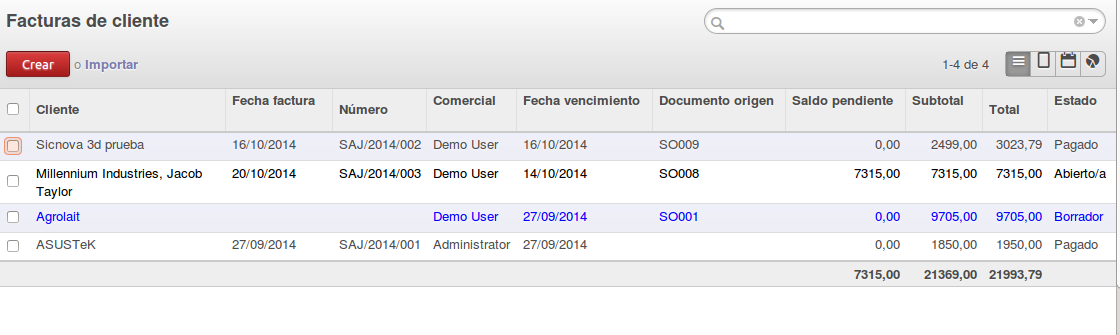
\includegraphics[width=\textwidth]{contabilidad/img/con_lisfact2.png}
\caption{Listado de facturas}
\label{con:lisfact}
\end{figure}


En el listado de facturas (figura \ref{con:lisfact} ) se ven los datos principales de las mismas. El \textbf{Cliente} al que hace referencia la factura, la \textbf{Fecha factura} de cuando fue creada, el \textbf{Número}, que no es más que la numeración de la factura, la cual es además personalizable. 

El \textbf{Comercial} hacereferencia a quién ha gerenardo la factura. Si la factura se crea a mano, este campo será el del usuario
que la ha creado. Si la factura ha sido generada automáticamente a través de una orden de venta, por ejemplo, este campo se rellenará con el nombre del comercial que ha generado dicha orden de venta. De igual manera, el campo \textbf{Documento origen} hará referencia a ese documento (orden de venta, por ejemplo) que ha generado automáticamente la factura.

La \textbf{Fecha de vencimiento} indica, en el caso de utilizar \emph{plazos de pago}. Esta fecha de vencimiento se genera automáticamente de acuerdo a estos plazos. Cuando se utilizan plazos de pagos, se generarán automáticamente los asientos contables en distintas fechas (para por  ejemplo pagos de 50\% en un plazo y el resto en otra fecha, adaptando este campo a estas fechas de asientos. También pueden no utilizarse plazo de pago y forzar una fecha de vencimiento concreta. O no utilizar ni fecha de vencimiento ni plazo de pago, indicando de esta manera que el pago es directo.

El \textbf{Saldo pendiente} indica el dinero pendiente de pago de esa factura. El campo \textbf{Subtotal} muestra el total a facturar \textbf{sin} contar con los impuestos, mientras que en el campo \textbf{Total} si muestra la facturación total incluyendo los impuestos.

El \textbf{Estado} de la factura, cuyos posibles estados son los siguientes:

\begin{itemize}
  \item \textbf{Borrador} -- Estado por defecto para las nuevas facturas. En este punto, las facturas \emph{son todavía editables en todos sus
                             campos}
  \item \textbf{Pro-forma} -- Si el sistema tiene activada la capacidad de generar facturas pro-forma, este estado se encontrará disponible. En
                             este punto, la factura no tiene aún una numeración asignada.
  \item \textbf{Abierto/a} -- En este estado, la factura está confirmada, y se mantiene en este estado hasta que se realiza el pago completo
                             de la misma. Al llegar a este estado, las facturas \emph{no permite editar todos sus campos}, no se pueden cambiar
                             las líneas de factura y otros elementos. Si fuera necesario cambiarlos, habría que \emph{Cancelar} la factura, editarla
                             y volver a aprobarla.
  \item \textbf{Pagada} -- Estado al que se llega automáticamente al introducir el pago (o los pagos) de la factura. Los asientos de estos pagos pueden
                           o no estar conciliados, esto no es relevante para el cambio de estado.
  \item \textbf{Cancelada} -- Estado al cancelar la factura. Las facturas canceladas que ya han sido numeradas (que han pasado por el estado de
                           abierto) \textbf{no pueden ser borradas}, hay que pasarlas a borrador, editarlas con la nueva información
\end{itemize}


\subsubsection{Factura individual}
\label{contabilidad:factura}
La figura \ref{con:facindividual} muestra la visión individual de una factura con su pestaña \emph{Líneas de factura} seleccionada. Además de esta pestaña hay otras dos denominadas \emph{Otra información} y \emph{Pagos}

\figura{contabilidad/img/con_facindividual.png}
{Vista individual de edición de una factura}
{con:facindividual}

Al seleccionar en el campo de \textbf{Cliente} uno ya existente, la factura se rellenará automáticamente con los datos de dirección y facturación introducidos en la ficha del cliente, no siendo necesario volver a repetirlos en la factura.

Se debe seleccionar la \textbf{Posición fiscal} si procede y añadirla fecha de la factura si no está completada (si no es una factura creada
automáticamente)

El campo de \textbf{Cuenta} se rellena automáticamente según el cliente, indica en que cuenta se crearán los asientos contables de esta factura  (no incluyendo los impuestos, por supuesto)

En la imágen se puede apreciar también la \textbf{pestaña Líneas de factura}. En esta pestaña se introducen las líneas de facturación, es decir, los productos incluidos en esta factura. Pulsando sobre el texto \emph{Añadir un elemento} se creará una nueva línea en la que se podrá elegir el producto a incluir a través de la columna \emph{Producto}. Al seleccionar el producto se rellenarán automáticamente el resto de campos. Estos se rellenarán con los datos introducidos previamente en el producto, pero pueden ser editados in situ en cada línea, por ejemplo. \textbf{A cada cambio que pueda afectar al precio} se debe, tras el susodicho cambio, pulsar en \emph{(actualizar)}, situado justo encima del calculo total de la cantidad de la factura.

Como \textbf{Plazos de pago} existen algunos por defecto, siendo totalmente configurable según las necesidades de la venta.

De igual forma, el campo de \textbf{Información adicional} se puede utilizar para almacenar cualquier información extra en relación a la factura.


\figura{contabilidad/img/con_pesotra.png}
{Pestaña \emph{Otra información} de una factura}
{con:pesotra}

La figura \ref{con:pesotra} muestra la \textbf{pestaña de \emph{Otra información}}. En la misma se puede observar algunos campos no relacionados de forma totalmente directa con la factura como el \textbf{Comercial} y \textbf{Equipo de ventas} responsables de la factura   el \textbf{Documento origen}-- rellenado automáticamente si la factura se genera automáticamente desde otro documento.

La \textbf{Referencia del cliente} es rellenada automáticamente en el caso de que exista dicha información en la ficha del cliente. De igual forma la \textbf{Cuenta bancaria}, campo que hace referencia al número de cuenta contra el que se pagará la factura, se extrae automáticamente de la ficha del cliente en el caso de que exista tal información con anterioridad. En cualquier otro caso siempre puede rellenarse en este punto.

El \textbf{Periodo contable} puede forzar a la factura a aparecer en determinado periodo contable si se elige alguno aquí. En caso contrario su periodo contable será asignado en función de la fecha de creación.

Los \textbf{Asientos contables}, que se aprecian vacios en la imagen, mostrarán un enlace a estos asientos en el momento en el que la facturasea validada.

Lo último que se puede observar es la \textbf{tabla de impuestos}. En ésta se reflejan los distintos impuestos que se han asignado en las líneas de factura indicando su descripción, la cuenta a la que apuntan los asientos de estos impuestos y la base y el importe del impuesto. Cada impuesto se representa en una línea distina.

\figura{contabilidad/img/con_pesasientos.png}
{Pestaña \emph{Pagos} de la factura}
{con:pesasientos}

La última pestaña es la \textbf{pestaña \emph{Pagos}}. En esta se presenta una tabla que contendrá la información de los pagos realizados para la factura. En esta se aprecia la \textbf{Fecha vigencia} y el \textbf{Asiento contable} asociado a ese pago. También el \textbf{Nombre} y \textbf{Referencia} del pago, información que se rellena cuando se crea este pago.

También aparece el \textbf{Diario} en el que se registra el pago y los campos \textbf{Debe} y \textbf{Haber} que complementan la información sobre el pago indicando la cantidad y dirección de la transacción de dinero.

\subsubsection{Pago de facturas}

La manera más cómoda de registrar los pagos de las facturas es a través de las mismas facturas. Cuando una factura ha sido validada, aparecerá un botón en la zona superior denominado \textbf{Registrar pago} tal como se aprecia en la figura \ref{con:facpagos}. Hacer click en este botón presentará la pantalla de registro de pago que se ve a continuación en la figura \ref{con:facpagar}

\figura{contabilidad/img/con_facpagos.png}
{Botones que aparecen en una factura abierta}
{con:facpagos}

\figura{contabilidad/img/con_facpagar.png}
{Diálogo para el registro de un pago}
{con:facpagar}

La mayoría de datos en el diálogo, se rellenarán de acorde a la información de la factura. El \textbf{Cliente} será el mismo que el indicado en la factura. El \textbf{Importe pagado} se rellenará automáticamente con el saldo pendiente de pago, pero modificable por el usuario. Mediante el \textbf{Método de pago} se indica la forma de pago, a través de banco, con efectivo\ldots

El resto de campos hacen referencia a la \textbf{Fecha} del pago, al \textbf{Periodo} al que pertenece el pago -- por defecto el actual aunque es modificable también por el usuario -- y una \textbf{Ref. Pago}, referencia personalizable del pago  y \textbf{Memoria}, campo también de uso personalizado. Cabe recalcar que estos dos últimos campos son opcionales.

En el momento en el que la suma de los pagos alcance el total de la factura, esta se considerará pagada automáticamente y los asientos serán conciliados.




\subsection{Facturas rectificativas de cliente}

Las \textbf{facturas rectificativas} son, en funcionamiento y en presentación, exactamente iguales que las facturas de cliente vistas en la sección anterior.

Cabe destacar que no es necesario, en la factura rectificativa, añadir cantidades en negativo. Al crear una factura rectificativa se da por sentado que las cantidades no son a cobrar por parte de los clientes, sino a reintegrar a los mismos. Esto quiere decir que una factura rectificativa que incluya, por ejemplo, una impresora, es señal de que se está haciendo una devolución de la misma por parte del cliente al que se le ha vendido -- todo en cifas positivas en la factura.

\subsubsection{Creación de facturas rectificativas}

La creación de facturas rectificativas puede hacerse de dos formas. La primera de ella es a través del botón \textbf{Crear} en la vista del listado de facturas rectificativas de cliente. Con este botón se creará una factura rectificativa vacia, a rellenar por completo por el usuario, incluyendo datos como el cliente, las referencias de la pestaña \emph{Otra información}, las líneas de productos\ldots

Una segunda forma de crear facturas rectificativas es a través del botón \textbf{Reintegrar factura} en las \emph{Facturas de clientes} -- no en las facturas rectificativas -- puede observarse en la figura \ref{con:facpagos} de la sección anterior. Aparecerá en las facturas validadas y abiertas y en las pagadas. Con este botón se presentará un diálogo (figura \ref{con:facrect}) en el que se indica como se reintegra la factura y como se rectificará.

\figura{contabilidad/img/con_facrect.png}
{Diálogo de creación de factura rectificativa}
{con:facrect}

Los campos obligatorios son, por un lado, el \textbf{Motivo}, de manera que se indique la razón de la rectificación de la factura, y el \textbf{Método de abono}, que determina como se crea la factura rectificativa. Las opciones de este método de pago y su funcionamiento son:

\begin{itemize}
  \item \textbf{Crear una factura rectificativa borrador} -- Crea una factura rectificativa en el estado de borrador para ser modificada por el
            usuario, pudiendo rectificar líneas de productos
  \item \textbf{Cancelar} -- Esta opción considera que la factura no debería haber sido creada, así pues, crea una factura rectificativa que
            anula aquella que se esté reintegrando, validandola y conciliando la factura de cliente y la rectificativa. La factura 
            rectificativa creada es automáticamente validada, no es posible editarla.
  \item \textbf{Modificar} -- Con la elección de esta opción se indica que se quiere modificar la factura. Como, en teoría, las facturas
            validadas y con una numeración asignada no pueden ser modificadas, esta opción crea una factura rectificativa que cancela -- 
            como la opción anterior -- la factura y las concilia y crea una nueva factura identica a la que se modifica en estado 
            de borrador. 
\end{itemize}






\subsection{Recibo de ventas}

Los recibos de ventas se utilizan para introducir los movimientos contables sin necesidad del uso de una factura. Serían los movimientos generados por un ticket de venta. 

Para estos elementos (puede verse una pantalla de edición en la figura \ref{con:recedita}) los datos mínimos necesarios son:

\begin{itemize}

  \item \textbf{Cuenta} -- Cuenta contable en la que se registrará el pago. Si se elige un cliente y se tiene configurada una cuenta para el
          mismo
  \item \textbf{Pago} -- Hay que indicar la forma de pago
      \begin{itemize}
         \item \textbf{Pagar directamente} -- Se interpreta que el pago ha sido inmediato
         \item \textbf{Pagar tarde o agrupar fondos} -- De esta manera se interpreta que el pago se realizará en una fecha determinada que se puede
              introducir bajo este campo (sólo aparecerá la opción de rellenar una fecha si se elige esta opción)
      \end{itemize}

  \item \textbf{Elementos de la venta} -- Se añaden en la pestaña de \textbf{Información de ventas}. Dentro de éste, hay que completar cuatro
 campos:
      \begin{itemize}
         \item \textbf{Cuenta} -- Cuenta contable referente a la venta (por ejemplo, la 7000000)
         \item \textbf{Descripción} --  Descripción de los productos que se venden.
         \item \textbf{Importe} -- Precio de la compra
         \item \textbf{Impuesto} -- En el caso de aplicar IVA a la compra, habrá que especificarlo en este campo
      \end{itemize}
\end{itemize}



\figura{contabilidad/img/con_recedita.png}
{Edición de un ticket de venta}
{con:recedita}


La creación de tickets de venta conlleva la creación de sus asientos contables correspondientes para ser asentados tras una supervisión de los mismos.




\subsection{Pagos de cliente}

Esta sección se encarga de mostrar -- y crear en caso necesario -- los pagos registrados en las facturas realizados por los clientes.

\figura{contabilidad/img/con_paglista.png}
{Listado de pagos de clientes}
{con:paglista}

De un vistazo se pueden observar los pagos realizados por los clientes, pudiendo determinar la \textbf{Fecha} de realización de los mismos, al igual que el \textbf{Número} que se asigna al pago.

También puede verse la \textbf{Empresa} responsable del pago, la \textbf{Referencia} si se ha introducido alguna, y el \textbf{total} del pago junto a su \textbf{Estado}, el cual puede variar entre estados \emph{Borrador}, \emph{Contabilizado} y \emph{Cancelado}.

\figura{contabilidad/img/con_pagindividual.png}
{Edición de un ticket de venta}
{con:pagindividual}

La información mostrada en una ficha individual de un pago (figura \ref{con:pagindividual} muestra la información sobre el cliente que realiza el pago, y las transacciones realizadas. Estas transacciones especifican el \textbf{Apunte contable} al que pertenece -- visible desde la pestaña \emph{Apuntes contables} de esa misma pantalla --, la \textbf{Cuenta} relacionada con la transacción, las \textbf{Fechas}, tanto de creación como de vencimiento y las diferencias en los \textbf{Saldos} con la transacción.

También puede verse si el asiento se encuentra conciliado al completo o no.


\subsubsection{Creación de pagos}

Desde esta misma sección se pueden crear esos pagos de clientes, no obstante, y debido a la complejidad relativa de esta pantalla, se aconseja -- en la medida de lo posible -- utilizar las funciones de registrar pagos desde las facturas. De esta manera se evitan posibles errores por despistes y asegura que todos los datos creados están relacionados y son consistentes.





\subsection{Clientes}
Los datos que se van a ver aquí son los mismos que se han explicado en la sección \ref{ven:clientes} (Vease esta sección para la explicación de estos datos)

Al seleccionar esta opción del menú, los datos presentados son aquellos clientes que tengan marcado, en la pestaña de ventas y compras de la ficha del mismo, la opción de \emph{Cliente}, situado encima de la otra opción \emph{Proveedor}. Se puede ver dicha opción en la imagen ref{con:fichacliente}

\figura{ventas/img/ven_cliventas.png}
{Ficha del cliente con la pestaña \emph{Ventas y compras}}
{con:fichacliente}











\section{Proveedores}

\subsection{Proveedores}
Los datos que se van a ver aquí son los mismos que se han explicado en la sección \ref{ven:clientes} (Vease esta sección para la explicación de estos datos)

Al seleccionar esta opción del menú, los datos presentados son aquellos clientes que tengan marcado, en la pestaña de ventas y compras de  la ficha del mismo, la opción de \emph{Proveedor}, situado bajo la otra opción \emph{Cliente}. Se puede ver dicha opción en la imagen \ref{con:fichacliente2}

\figura{ventas/img/ven_cliventas.png}
{Ficha del cliente con la pestaña \emph{Ventas y compras}}
{con:fichacliente2}


\subsection{Otras secciones de proveedor}

El resto de secciones en el área de proveedores corresponden a exactamente lo mismo que en el área de clientes, pero con la orientación contraria. 

Esto último quiere decir, obviamente, que las \textbf{Facturas de proveedor} y \textbf{Facturas rectificativas de proveedor} es la información de las facturas realizadas a nuestra empresa por parte de los proveedores. El formato de las mismas para insertarlas aquí es exactamente el mismo que en las facturas que se realizan a los clientes. El software se encargará de que el IVA (por ejemplo, además de otros campos) se dirija a la cuenta adecuada, al IVA de las compras.

Los \textbf{Recibos de compra} son los tickets de compra de distintos elementos (como pueda ser gasolina sin facturar o pequeñas comprar en comercios donde no realicen factura) Se insertan de igual manera que los \emph{Recibos de ventas}

La sección de \textbf{Pagos a proveedores} aglutina las distintas transacciones realizadas hacia los proveedores de igual manera que en \emph{Pagos de cliente} se pueden observar todos los pagos de los clientes hacia nuestra empresa de un solo vistazo.








\section{Banco y caja}
\subsection{Extractos bancarios}
El software permite la introducción y almacenaje de los extractos bancarios. Cuando se edita un extracto se puede ver la pantalla
representada en la figura \ref{con:banextractos}.

Con el \textbf{saldo inicial} introducido, el \textbf{saldo final} es calculado en función de las transacciones introducidas en el 
extracto.

Cabe la posibilidad de insertar cada transacción a mano en las líneas inferiores o bien utilizar el botón \textbf{Importar Facturas}, desde la cual se pueden seleccionar facturas pendientes de cobro o de pago. Con esta acción, se añadirán automáticamente líneas en el extracto con la información de la factura. Por defecto, en el extracto se supone que se paga toda la factura (o lo que queda por pagar de la misma), pero es modificable por el usuario. En el caso de que se realice un pago que complete la factura, se indicará mediante un icono verde a la derecha de la línea, mientras que si no concilia por completo el pago, lo mostrará con un icono rojo.

Cuando el extracto es confirmado, se generarán los asientos a los que hace referencia el extracto, con las cantidades, cuentas y clientes indicados en las lineas del mismo.

\figura{contabilidad/img/con_banextractos.png}
{Extracto bancario}
{con:banextractos}



%\subsection{Registros de caja}







\section{Asientos contables}

\subsection{Apuntes contables}
\figura{contabilidad/img/con_apuapuntes.png}
{Listado de apuntes contables}
{con:apuapuntes}

En la pantalla de apuntes contables se presentará, en forma de listado y filtrado por \textbf{Periodo} y \textbf{Diario} -- como se aprecia en la parte superior izquierda del mismo listado -- todos los apuntes contables (figura \ref{con:apuapuntes})



Desde este mismo punto es posible crear nuevos apuntes contables pulsando sobre el boton \textbf{Crear} y rellenando todos los datos adecuadamente. Hay que tener claro que siempre se ha de situar el mismo valor en el campo \emph{Asiento contable} si lo que se está creando son las partidas y contrapartidas de un asiento ya que sólo se consideran como parte de un mismo asiento, si coinciden en este campo. En caso contrario se entienden como apuntes sueltos, no relacionados con ningún asiento.	



\subsection{Asientos contables}

La opción de \emph{Asientos contables} mostrará todos los asientos, sin filtrar ni por periodo ni por diario como en el caso de los apuntes. La figura \ref{con:apuasientos} muestra la presentación de los mismos.

\figura{contabilidad/img/con_apuasientos.png}
{Listado de asientos contables}
{con:apuasientos}

Los campos que se pueden ver son:

\begin{itemize}
  \item \textbf{Nombre} -- Nombre del apunte
  \item \textbf{Referencia} -- Referencia que puede apuntar a facturas u otros documentos.
  \item \textbf{Fecha} -- Fecha de creación del apunte
  \item \textbf{Periodo} -- Periodo del ejercicio fiscal al que pertenece el apunte.
  \item \textbf{Diario} -- Diario en el que se introduce el apunte.
  \item \textbf{Empresa} -- Empresa cliente (o proveedor) relacionada con esta entrada.
  \item \textbf{Importe} -- Valor total del importe contenido en el apunte.
  \item \textbf{A revisar} -- Permite marcar el asiento en el estado "A revisar" para que un supervisor encargado lo revise dado el caso.
                            No tiene efecto sobre el asiento en ningún aspecto, tan sólo lo etiqueta para su revisión posterior.
  \item \textbf{Estado} -- Estado en el que se encuentra el asiento. En este caso sólo hay dos estados
     \begin{itemize}
       \item No asentado
       \item Asentado
     \end{itemize}
\end{itemize}

Bien utilizando el botón \textbf{Crear} o pulsando sobre uno de los asientos, se puede acceder para ver y editar -- en el caso de que no se encuentre asentado -- cualquier asiento individual. Lo que el usuario verá está presentado en la figura  \ref{con:apuasientoeditar}

\figura{contabilidad/img/con_apuasientoeditar.png}
{Listado de asientos contables}
{con:apuasientoeditar}

El \textbf{Diario} y el \textbf{Periodo} son seleccionables por el usuario y obligatorios. El campo de \textbf{Referencia} es opcional, es autorellenado en caso de que el asiento sea creado automáticamente a partir de una factura o algún otro documento, al igual que los campos de \emph{Diario} y \emph{Periodo}.

En la pestaña de \textbf{Apuntes contables} se pueden ver e introducir los apuntes correspondientes al asiento, los campos a rellenar de los que se dispone son:

\begin{itemize}

  \item \textbf{Nombre} -- El nombre del apunte.
  \item \textbf{Empresa} -- Empresa relacionada con el apunte. No es obligatoria.
  \item \textbf{Cuenta} -- Cuenta a la que hace referencia esa línea de apunte.
  \item \textbf{Fecha de vencimiento} -- Fecha límite para el pago de la línea.
  \item \textbf{Debe -- Haber} -- Campos para introducir la información de Debe y Haber del apunte.
  \item \textbf{Importe divisa} -- En el caso de un asiento multidivisa, aquí debe insertarse el valor de la misma.
  \item \textbf{Cuenta impuesto} -- Cuenta de un impuesto a la que hace referencia el apunte. En este caso hace referencia al código del impuesto, no a la cuenta del mismo (la cual se insertaría en el campo \emph{cuenta}).
  \item \textbf{Importe Impuesto/base} -- Se introduce el valor del monto del impuesto o la base impositiva en función del tipo de cuenta. En el caso de cuentas de tipo impositivo, se utiliza el monto del impuesto. En caso contrario introduce el monto de la base imponible.
  \item \textbf{Estado} -- No es editable por el usuario. Indica si el apunte está cuadrado o no, pudiendo saber si el asiento cuadra finalmente.
  \item \textbf{Conciliar} -- No editable por el usuario. Cuando se realiza la conciliación de los apuntes, se indica en este campo la referencia a la conciliación.
  \item \textbf{Conciliación parcial} -- No editable por el usuario. Igual que en el caso anterior, pero se aplica en el caso de conciliaciones parciales.
\end{itemize}


%\subsection{Diarios de comprobantes}







\section{Planes contables}

Las opciones disponibles  en esta sección se encargan de generar las tablas, en formato legible en pantalla sobre el plan contable actual y sus cuentas y la información sobre impuestos que se encuentra en la contabilidad de la base de datos.

\subsection{Plan contable}

Para la obtención del plan se presenta un diálogo en el que se selecciona tanto el ejercicio fiscal como el rango de \textbf{periodos} entre los que se quiere obtener la información, seleccionando además si para este informe se utilizará la información contenida sólo en los
asientos asentados o la información de todos los asientos -- no asentados incluidos.

El diálogo para la configuración del plan se puede ver en la figura \ref{con:plancontable} y la presentación en pantalla del mismo se puede ver en la figura \ref{con:plancontablefinal}

\figura{contabilidad/img/con_plancontable.png}
{Diálogo para la creación del plan contable}
{con:plancontable}

\figura{contabilidad/img/con_plancontablefinal.png}
{Presentación en pantalla del plan contable}
{con:plancontablefinal}

Si en alguna de las líneas que se ven en el plan contable, se hace click, se abrirá para ver en mayor detalle los asientos correspondientes a esa cuenta seleccionada.

\subsection{Impuestos}

De igual manera que en la sección anterior, al acceder a esta opción se presenta un diálogo para definir que impuestos analizar. La elección en este caso se reduce a un \textbf{periodo} (trimestre, mes...) En caso de que se deje vacio ese campo, el informe se hará  analizando todos los periodos que no esten cerrados.

Otra opción disponible es, al igual que en el informe del plan contable, si para la creación del informe se tendrán en cuenta los asientos asentados o todos, inclusive los que no están asentados (Opción \textbf{Movimientos destino}

En las siguientes figuras se puede ver el diálogo para definir el informe (\ref{con:planimpuestos}) y la presentación en pantalla de la información (\ref{con:planimpuestosfinal})

\figura{contabilidad/img/con_planimpuestos.png}
{Diálogo para la obtención del informe de impuestos}
{con:planimpuestos}

\figura{contabilidad/img/con_planimpuestosfinal.png}
{Presentación en pantalla del informe sobre impuestos}
{con:planimpuestosfinal}

Además, haciendo click sobre alguno de los impuestos, se abrirá en más detalle los movimientos (asientos) relacionados con ese impuesto.


\section{Procesamiento periódico}


\subsection{Asientos Borrador}
\label{con:asentar}
La única opción dentro de esta subsección es \textbf{Asentar asientos}. Como su propio nombre indica, es una utilidad para asentar todos esos asientos que no se encontraran ya en ese estado.

Esta opción abrirá un diálogo (figura \ref{con:aseasientos}) a través del cuál se seleccionará el \textbf{Diario} de asientos que se quiere asentar y el \textbf{periodo}. Tras seleccionar ambos elementos se asentarán todos esos elementos que entren dentro 
de las opciones seleccionadas.

\figura{contabilidad/img/con_aseasientos.png}
{Dialogo de asentamiento de asientos}
{con:aseasientos}



\subsection{Conciliación}

\subsubsection{Conciliación manual}

En esta opción se presentará una lista de todos los movimientos (asientos) no conciliados, organizados por empresas a las que pertenecen estos movimientos. La vista general es la que se observa en la figura \ref{con:conmanual}

\figura{contabilidad/img/con_conmanual.png}
{Pantalla de conciliación manual}
{con:conmanual}

A través de esta pantalla se pueden seleccionar distintos asientos no conciliados y aceptar la conciliación entre ellos. Cuando esta selección y acción se realiza, aparece un diálogo para la confirmación de la conciliación (figura \ref{con:conmanuald1})

\figura{contabilidad/img/con_conmanual_d1.png}
{Diálogo de conciliación manual}
{con:conmanuald1}

Si el importe del desajuste fuese igual a cero, se permitiría realizar una \textbf{Conciliación total}. En el caso de que no lo sea -- como en el ejemplo --, puede realizarse una conciliación parcial o una conciliación con desfase. La \textbf{Conciliación parcial} se utiliza si el cliente va a pagar sólo parte de la factura, dejando conciliados los asientos. Con la \textbf{Conciliación con desfase} crea un movimiento de desajuste para su conciliación a posteriori.

Con la opción de \emph{Conciliación con desfase} se presentará a su vez un diálogo para crear ese Movimiento de desajuste, diálogo que es exactamente igual que la parte inferior del diálogo de conciliación automática (figura \ref{con:conauto}). En este diálogo se completa la información sobre ese movimiento, la cuenta, diario y periodo en el que se creará el desajuste.


\subsubsection{Conciliación automática}
Para que una factura se considere pagada, los apuntes contables de la mismas deben estar conciliados con sus contrapartidas, normalmente pagos. Con esta función de conciliación automática, el programa realiza una búsqueda de apuntes a conciliar en las cuentas en las que se le indica. Encuentra los apuntes, de acorde a las empresas, cuando las cantidades se corresponden realiza la conciliación de esos apuntes. 

La siguiente figura muestra el diálogo de conciliación automática.

\figura{contabilidad/img/con_conauto.png}
{Diálogo de conciliación automática}
{con:conauto}

En el área superior y mediante el botón \textbf{Agregar}, se añaden las cuentas en las que se realizará la busqueda de asientos a conciliar. Como se puede apreciar, muestra información sobre esas cuentas, incluyendo entre otras, información sobre el \textbf{debe} y el \textbf{haber}, mostrando también el \textbf{saldo pendiente}.

El campo \textbf{Fuerza} se refiere al número de importes parciales máximo que pueden agruparse para encontrar una conciliación. Esto quiere decir que, en función de todos los asientos disponibles, los combinará entre ellos (con un máximo de elementos combinados definidos por este campo) para comprobar cuales cuadran para ser conciliados.

Si se selecciona la opción \textbf{Permitir desfase}, creará una entrada en la \emph{cuenta}, \emph{diario} y \emph{periodo} indicados en la parte inferior del diálogo -- la parte bajo el nombre \textbf{Movimiento de desajuste} -- donde también se puede indicar el importe máximo para el que se puede crear esa entrada de desajuste.




\subsection{Asientos recurrentes}

En esta sección se pueden definir y generar asientos que se repitan en el tiempo. Pueden categorizarse aquí elementos como algunos alquileres o gastos que se conocen fijos cada cierto periodo de tiempo.

\subsubsection{Definir asientos recurrentes}

La pantalla a la que se accede a través de ésta sección muestra la lista de asientos que se repiten a lo largo del tiempo. Cada una de estas entradas es accesible de forma individual, pudiendo verse la pantalla como la que se muestra en la figura \ref{con:reclista}.

\figura{contabilidad/img/con_reclista.png}
{Edición de asiento recurrente}
{con:reclista}

En la creación de estos asientos recurrentes es necesario el uso de un \textbf{modelo} (que se puede ver más adelante), usar un \textbf{Nombre} para referenciarse al mismo, e indicarle una \textbf{Fecha inicial}, una \textbf{unidad de tiempo} y un \textbf{ periodo} (cada cuantas unidades de tiempo se repetirá el asiento) además del \textbf{número de periodos}, es decir, el número de repeticiones.

Cuando todas esas opciones se encuentran seleccionadas, se puede hacer uso del botón \textbf{Calcular}. Este botón creará los apuntes (que no los asientos) periódicos y los mostrará en la lista inferior (\emph{Apuntes de asientos periódicos}). El ejemplo anterior mostraría lo que se ve en la figura \ref{con:reclistacal}.

\figura{contabilidad/img/con_reclistacal.png}
{Apuntes de asientos periódicos calculados}
{con:reclistacal}

Sin embargo, se aprecia que los campos \emph{Asiento} no está completado. Con esto, se ha calculado donde estarán los asientos, no los asientos en sí. Para generarlos, debe usarse la siguiente opción en el menú (\emph{Generar asientos}). Una vez generados, se enlazarán en estos campos del listado.

De igual manera, se puede seleccionar, pulsando sobre el apunte en la lista, un asiento ya creado.


\subsubsection{Generar asientos}

Esta opción mostrará el diálogo que se aprecia en la figura \ref{con:recgenerar}. Mediante este, se selecciona una fecha \textbf{hasta la cual} se generarán todos los asientos de los asientos recurrentes que no tengan creados esos asientos. 

Siguiendo el ejemplo anterior, utilizar la fecha a tres meses de la actual, generará tres asientos de alquiler, que además se reflejará en la lista de apuntes del asiento recurrente (el listado visto en la figura \ref{con:reclistacal})

\figura{contabilidad/img/con_recgenerar.png}
{Diálogo de generación de asientos}
{con:recgenerar}


\subsubsection{Modelos}

Los modelos hacen referencia a las entradas del asiento que compondrán cada asiento recurrente. Para el ejemplo del alquiler, se rellenarían los datos tal y como se haría para crear los asientos referidos a un alquiler. Con ello, cada vez que se cree un asiento de este modelo, ese asiento contendrá únicamente esos datos, con las fechas adecuadas en cada caso.


\figura{contabilidad/img/con_recmodelo.png}
{Edición de un model de asiento recurrente}
{con:recmodelo}




\subsection{Fin de periodo}

\subsubsection{Cerrar un periodo}
A través de este elemento, se presentará un listado de los periodos actualmente abiertos (figura \ref{con:finperiodo}). En esta lista se puede seleccionar uno o varios periodos y utilizar el menú desplegable \emph{Más} para seleccionar la opción \textbf{cerrar}.

Otra opción es entrando en la visión individual de periodo, haciendo click sobre el que se desée en la lista, y utilizar el botón \textbf{Cerrar periodo} que aparece en la ficha del mismo.

\figura{contabilidad/img/con_finperiodo.png}
{Listado de periodos a cerrar}
{con:finperiodo}


\subsubsection{Generar asientos de apertura}
Esta opción del menú mostrará un diálogo para generar los asientos de apertura de un ejercicio fiscal en base a los datos del
ejercicio fiscal anterior.

Se ha de indicar el \textbf{ejercicio a cerrar} y el \textbf{ejercicio a abrir}, además de el \textbf{diario} y \textbf{periodo} en 
los que se crearán los asientos de apertura, pudiendo además añadirle un \textbf{Nombre} a esos asientos para poder 
identificarlos apropiadamente.

\figura{contabilidad/img/con_finapertura.png}
{Diálogo de generación de asientos de apertura}
{con:finapertura}



\subsubsection{Cancelar apuntes de cierre}

Esta opción del menú abrirá el diálogo que permite cancelar los apuntes de cierre del año fiscal. Sólo será necesario indicarle
el año fiscal del que hay que cancelar los asientos

\figura{contabilidad/img/con_fincancelar.png}
{Diálogo de cancelación de asientos de cierre}
{con:fincancelar}



\subsubsection{Cerrar un ejercicio fiscal}

Cierra un ejercicio fiscal. El diálogo sólo requerirá de indicarle que ejercicio es el que se debe cerrar.

\figura{contabilidad/img/con_fincierre.png}
{Diálogo de cierre del año fiscal}
{con:fincierre}









\section{Informe}

Este menú permite la generación de distintos informes sobre la contabilidad de la empresa agrupando los datos según los mismos. Genera un archivo PDF en cada ocasión.

Para generar los distintos informes, todos siguen un patrón relativamente fijo al poder filtrar los resultados por fecha, por periodos o por otros parametros como -- por ejemplo en los balances -- aquellas cuentas cuyo total no sea cero.

Cada una de las opciones de informes abrirá una ventana emergente con las distintas opciones para la generación de dichos informes. Generar los informes no modifica ninguna información existente en la base de datos, pudiendo por lo tanto generar todos los que sean necesarios sin temor a modificar nada.

%\subsection{Informes legales}
%\subsubsection{Informes contables}
%\subsubsection{Diarios}

%\subsection{Informes genéricos}
%\subsubsection{Empresas}
%\subsubsection{Impuestos}


%
% Este archivo es parte de un documento sobre OpenERP/Odoo creado
% y distribuido bajo licencia GNU Free Documen License v1.3.
%
% Para obtener la fuente e información más detallada, visite
% https://github.com/Gabriel-fm/oerp-manual
%
% Copyright (c) 2014 - Gabriel Franco
%


\chapter{Módulo de Almacén}
\label{moduloAlmacen}
El stock es la parte física de sus productos, cosas más que datos. Por ello, necesitan ser almacenados y trasladados entre ubicaciones, y hacer un seguimiento en grupos e individualmente. Tienen un tamaño, un peso y un coste. OpenERP gestiona todo este de una manera única y práctica.

La gestión del stock por OpenERP es muy simple, flexible y completa. Se basa en el concepto de la doble entrada que \emph{revolucionó} la contabilidad. El sistema puede ser descrito por la máxima de Lavoisier “nada perdido, todo cambiado” o, mejor, “todo  se movió”. En OpenERP no se habla de desaparecer, consumir o perdida de productos: en su lugar se habla sólo de movimientos de stock de un lugar a otro.


Al igual que en contabilidad, OpenERP gestiona contrapartidas para cada una de sus operaciones como recibos de proveedores, envío a clientes, beneficio y perdidas de inventario y consumo de materiales. Los movimientos de stock siempre se hacen de una ubicación a otro. Para satisfacer esta necesidad de una contrapartida para cada movimiento de stock, el software permite distintos tipos de ubicación para el stock.

\begin{itemize}
\item Ubicaciones físicas del stock
\item Ubicaciones de cliente
\item Ubicaciones virtuales como contrapartida para la producción e inventario
\end{itemize}

Las ubicaciones físicas representan almacenes físicos y su estructura jerárquica. Estos son generalmente las ubicaciones que son manejadas por los sistemas de stock tradicionales.

Las ubicaciones de los clientes representan los stocks de sus clientes y proveedores. Para seguir con la analogía de contabilidad, estos almacenas representan el papel de las cuentas de terceros. Recibir de un proveedor puede mostrarse como un movimiento de bienes de una ubicación de otra empresa a una ubicación física en su propia compañía. Como ve, las ubicaciones de proveedor muestran normalmente un stock negativo y las ubicaciones de cliente tendran un stock positivo.


Las ubicaciones virtuales como contrapartida para la producción, son utilizadas en las operaciones de manufactura. Manufacturar se caracteriza por el consumo de materiales y la producción de productos finales. Las ubicaciones virtuales se usan como contrapartida de estas dos operaciones. En el caso que nos concierne, no trataremos con ellas.


Las ubicaciones del inventario son contrapartidas de las operaciones del stock, representando los beneficios y perdidas de su compañía en términos de stock.

En OpenERP, las ubicaciones se estructuran jerárquicamente. Puede estructurar sus ubicaciones como un árbol o con relaciones padre-hijo. Esto brinda niveles más detallados de análisis de sus operaciones de stock y de la organización de su almacén.

En OpenERP un Almacén representa el lugar donde su stock físico se encuentra almacenado. Un Almacén puede estructurarse en varias ubicaciones y multiples niveles. Las ubicaciones se usan para gestionar todo tipo de lugares de almacenamiento, tal como las contrapartidas del cliente y producción.



\section{Conceptos en gestión de stock}
Para mostrar el concepto de gestión de stock veremos como se generan los movimientos de stock a través de las siguientes operaciones:

\begin{itemize}
\item Recibir productos de un proveedor
\item Envíos a clientes
\item Operaciones de inventario para materiales perdidos
\end{itemize}

Estos movimientos se muestran en tablas para hacerlo visualmente más comprensible:

\begin{table}[!th]
\begin{center}
\begin{tabular}{|c|c|}
  \hline
  Ubicación & Productos \\
  \hline
  Ubicaciones $>$ Proveedores & -30 bicicletas \\
  \hline
  Ubicaciones físicas $>$ Su empresa $>$ Stock & +30 bicicletas \\
  \hline
  
\end{tabular}
\end{center}
\caption{Compra de stock}
\label{al:compra}
\end{table}

En la tabla \ref{al:compra} se observa como al obtener stock, se muestra la aparición del mismo en las instalaciones de la empresa, mientras que aparece la cantidad equivalente, pero en negativo, en las ubicaciones del proveedor. Esto muestra como el proveedor se deshace de dos bicicletas mientras que en nuestro almacén aparecen dos bicicletas. El resultado de la operación, si todo está correcto y el stock se mueve de forma correcta es que todo suma siempre cero. 

De forma equivalente a esto, se realizan los movimientos de stock hacia los clientes como se muestra en la tabla \ref{al:venta} a continuación

\begin{table}[!th]
  \begin{center}
  \begin{tabular}{|c|c|}
    \hline
    Ubicación & Poductos \\
    \hline
    Ubicaciones físicas $>$ Su compañia $>$ Stock & -2 bicicletas \\
    \hline
    Ubicaciones clientes $>$ Clientes europeos & +2 biciletas \\
    \hline
  \end{tabular}
  \end{center}
  \caption{Venta de stock}
  \label{al:venta}

\end{table}

Así puede ver que la suma de stocks de un producto en todas las ubicaciones de OpenERP es siempre cero. En contabilidad se diría que la suma de débitos es igual a la suma de créditos.

Las ubicaciones de las empresas (de clientes y proveedores) no se localizan jerárquicamente bajo su empresa, así pues sus contenidos no se consideran parte de su stock. Así que si mira en la ubicación física dentro de su compañía, esas dos bicicletas no están más en su compañía. Aunque no se encuentren en su stock físico, es todavía muy útil el verlos en el stock de su cliente, ya que ayudará a llevar un análisis de la gestión de stock detallada.

En la gestión del stock, es complicado evitar un salto entre los datos en el software y las cantidades reales en el stock. La gestión de doble entrada del stock da el doble de oportunidades para encontrar un error. Si olvida dos items del stock, este error se reflejará automáticamente en la ubicación de la contrapartida.


Puede realizar una comparación con contabilidad, ya que podrá encontrar errores fácilmente ya que puede buscar errores en las cuentas propias o en las contrapartidas: si no hay suficiente en la cuenta del banco es, probablemente, porque alguien olvidó introducir el pago de una factura de cliente. Sabe que siempre la suma de debitos debe ser igual a la suma de créditos tanto en contabilidad como en la gestión de stock de OpenERP.
En contabilidad, todos los documentos apuntan a entradas de contabilidad que forman la base de la gestión contable. Si crea facturas, por ejemplo, los resultados de las operaciones son entradas de contabilidad en las cuentas. Y de igual forma para la gestión del stock en OpenERP. Todas las operaciones de stock se llevan a cabo como movimientos de stock. Ya si empaqueta productos o los manufactura o realiza una operación sobre el inventario en el stock, los movimientos de stock lo reflejarán en todo momento.


Se ha visto un ejemplo simple de recepción de bienes y envío de productos, pero algunas operaciones son menos obvias – una operación de inventario en el stock, por ejemplo. Una operación de inventario se lleva a cabo cuando se compara el stock mostrado en el software con los productos reales contados en los almacenes.

En OpenERP, con su gestión de doble entrada de stock, debería usar los movimientos de stock para estas operaciones de inventario. Esto ayudará a la trazabilidad del stock. Suponga que hay 26 bicicletas en el stock real, pero OpenERP muestra 28 en el sistema. Debe pues, reducir el número en OpenERP a 26. Esta reducción de 2 unidades se considera una perdida o destrucción de productos y la corrección se realiza con la siguiente operación:

\begin{table}[!th]
\begin{center}
\begin{tabular}{|c|c|}
  \hline
  Ubicación & Productos \\
  \hline
  Ubicaciones físicas $>$ Su empresa $>$ Stock & -2 bicicletas \\
  \hline
  Ubicaciones virtuales $>$ Perdidas de inventario & +2 bicicletas \\
  \hline
\end{tabular}
\end{center}
\caption{Operación de ajuste de stock}
\label{al:perdidas}
\end{table}

Después de unos meses, usted puede realizar evaluaciones del stock en la ubicación a través de Control de Inventario $>$ Estructura de ubicaciones $>$ ubicaciones virtuales $>$ Perdidas de inventario. Esto le dará el valor de perdidas de stock de la compañía en un periodo dado.

Una vez comprendido como funciona la gestión de stock en OpenERP, se puede pasar al analisis de cada elemento del módulo de Almacén.


\section{Recepción/Envios por Pedidos}
En esta parte del módulo de gestión de almacén se lleva el control del movimiento de stock desde y hacia la compañia. Se entiende cada uno de los movimientos en esta sección como un albarán en el que se engloba, como un único pedido, varios productos.

La creación de estos albaranes puede ser tanto manual como automática. La creación automática de estos albaranes viene en consecuencia de la creación de ordenes de venta a clientes y pedidos de compra a proveedores. Estas acciones, aparte del movimiento económico que conllevan, implican un cambio en el stock de la empresa, tanto una minimización del mismo en las ventas como un engrosamiento en el caso de compras. También existen albaranes de movimientos de stock internos en el caso de que la compañia mantenga varias ubicaciones físicas de stock, controlando en cualquier caso qué y cuánto material hay en cada sitio.

En el caso de las ventas, cuando alguién en la sección ventas lleva a cabo el proceso comercial con éxito, resultando en la facturación al cliente, con la aprobación de la venta se generará a su par un albarán de salida en el que estarán reflejados los productos que han sido vendidos en esa transacción, a qué cliente se envían y el resto de datos relacionados con el proceso. De esta manera, el encargado de almacén, tan sólo tiene que estar atento a esta, su sección, para saber que materiales deben salir del almacén y a que dirección han de ser enviados. De igual manera, al realizar una compra, el encargado sabrá que ha de haber una recepción de material, especificando cuál y cuánto, para poder confirmar que la compra se ha realziado con éxito.



\subsection{Albaranes de entrada}
\subsubsection{LISTADO DE ALBARANES}

\begin{figure}[H]
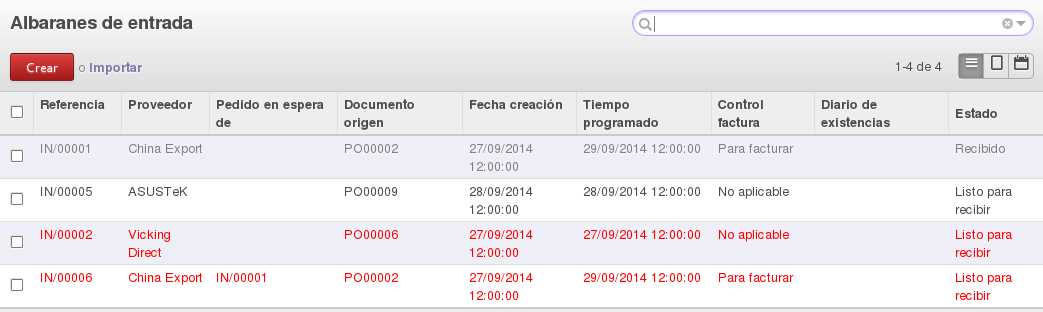
\includegraphics[width=\textwidth]{almacen/img/alb_entrada.png}
\caption{Albaranes de entrada}
\end{figure}

Al entrar en la sección de albaranes de entrada, se ofrecerá una visión general de todos los albaranes para los pedidos entrantes en sus distintos estados. En una visión general, los distintos campos representados serán:

\begin{description}
  \item[Referencia] 
    Una referencia a este albarán/pedido. Usado para control interno. 
  \item[Proveedor] 
    Proveedor del que se espera la recepción de material.
  \item[Pedido en espera de]
    Este campo es usado en caso de que se realicen recepciones parciales de material. Si cuando se espera un pedido, se recibe sólo una parte del mismo, al indicar que parte de material se recibe, se crea un segundo albarán que contendrá el resto de materiales a recibir, indicando en este campo de que albarán original depende ese material a recibir.
  \item[Documento origen] 
    Cuando se realizan los pedidos desde las ordenes de compra u otros lugares, este campo hace referencia a ese documento que originó la recepción de material. En el caso del ejemplo se puede ver que los albarances tienen como documento de origen pedidos de compra.
  \item[Fecha de creación] 
    Fecha en la que se creó el albarán.
  \item[Tiempo programado] 
    Fecha en la que se espera la recepción del producto. Para el cálculo de la misma se tiene en cuenta los datos ya introducidos en el proveedor y en los productos, en los que se puede indicar los tiempos de espera que suelen tener ese proveedor/producto.
  \item[Control factura] 
    Especifica el estado de facturación del pedido. Este campo también dependerá de como se haya generado el pedido. Hay pedidos que pueden facturarse una vez recibidos y habrá pedidos que se facturen antes de ser recibidos. En la captura del ejemplo se puede observar como una de las recepciones está lista para facturar, mientras que el resto la factura es a priori.
  \item[Diario de existencias] 
    En este campo se especifica si el albarán/pedido es parte de algún diario de existencias. Estos \emph{diarios} sirven para aglutinar distintos albaranes bajo la responsabilidad del dueño del diario. Si existen responsables distintos para la recepción de diferentes productos, se puede especificar en este campo. 

Esto es útil a efectos de análisis de responsabilidades en el caso de tener diferentes responsables de materiales en almacén. También puede utilizarse para indicar quién es el encargado de la recepción de ese pedido en el momento de llegada. Usarlo de una u otra manera queda en función de como gestione la empresa el almacen.
  \item[Estado] 
    Estado del albarán. Este puede variar entre distintos estados. Los habituales en este caso son \emph{Recibido} y \emph{Listo para recibir}.
\end{description}

\vspace{0.5cm}


\subsubsection{Vista de un albarán}

En la lista anterior, al hacer click sobre alguna linea de albarán, se pasará a la vista de un albarán y sus contenidos, de manera más especifica que la visión en la lista. En este punto se detallará el contenido esperado del pedido y más especificaciones.

\begin{figure}[H]
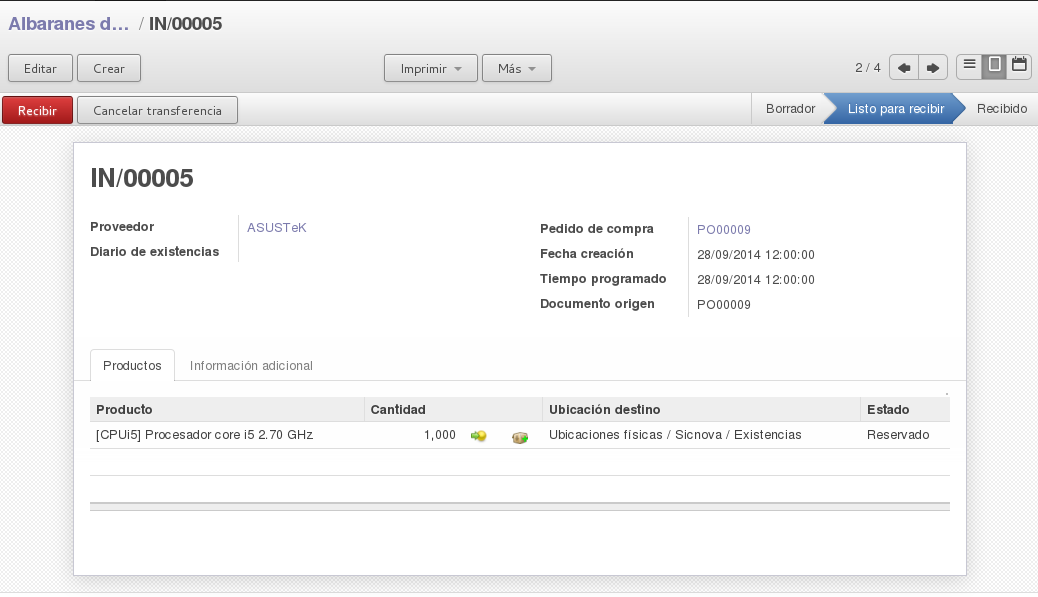
\includegraphics[width=\textwidth]{almacen/img/alb_entrada_i.png}
\caption{Albarán de entrada individual}
\end{figure}

En la parte superior del albarán individual se pueden observar los campos que se veían cuando se abría la lista de albaranes de entrada.

En la parte inferior se pueden observar dos pestañas. La primera de ellas es \textbf{Productos}. En esta pestaña se listarán los productos que se esperan de ese pedido. En cada una de las lineas se especificará uno de los productos a recibir y los elementos de cada línea se componen de los siguientes elementos:

\begin{description}
  \item[Producto] Se especfica el nombre del producto y su referencia según se ha especificado al crear el producto.

  \item[Cantidad] Indica el número de productos de ese tipo a recibir en la recepción de este albarán.

  \item[Botón de deshechar productos] Con este botón se pueden pasar productos de la recepción a una ubicación virtual denominada \emph{Productos deshechados} que indicarían que tales productos no han sido validos y han sido deshechados.

Con esta acción se abrirá una nueva ventana emergente en la que se preguntará que cantidad de producto es la que va a ser deshechada y permitirá indicar en que ubicación de almacén de deshecho se registrará el movimiento de stock (en caso de que haya varias)

  \item[Botón Poner en un nuevo paquete] Permite indicar que cierta parte del pedido de ese producto en concreto llegará o ha llegado en un nuevo paquete.

Al seleccionar esta opción se abrirá una ventana emergente en la que se preguntará que cantidad del producto elegido \textbf{se quedará} en el albarán actual.

  \item[Ubicación destino] Este campo describe en que ubicación del almacén será el que albergue los productos una vez sean recibidos.

  \item[Estado] Indica, en ese producto, cuál es su estado en el stock. Esto quiere decir que ese producto que se va a recibir puede tener alguno de los siguientes estados:

    \begin{description}
    \item[Reservado] \hfill \\ Cuando los productos a recibir están reservados quiere decir que existe otro movimiento (normalmente una venta) que está a la espera de recibir stock de ese producto para poder ser realizado
    \item[Esperando disponibilidad] \hfill \\ Si el producto está en este estado es que simplemente está a la espera de la recepción del paquete. Una vez que el paquete se recibe se supone que este producto está disponible. En este caso el producto no se encuentra reservado ni pedido por otra transacción de almacén.
    \end{description}
\end{description}

\vspace{0.5cm}

La pestaña \textbf{Información adicional} contiene algunos datos extra sobre la recepción del pedido, algunos de los cuales pueden ser modificados por el responsable de almacén si se da el caso.

\begin{figure}[H]
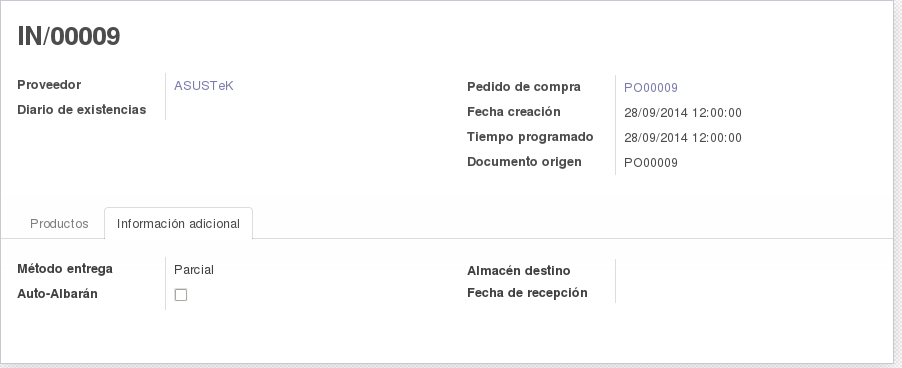
\includegraphics[width=\textwidth]{almacen/img/alb_entrada_m.png}
\caption{Pestaña de información adicional}
\end{figure}


\begin{description}
  \item[Método de entrega] Puede ser \textbf{Parcial} si se puede recibir en varias partes los distintos productos, o \textbf{Todo junto} si la recepción se realiza en un solo paquete.
  \item[Auto-Albarán] Esta opción es creada cuando se utiliza OpenERP para la manufactura de productos. Añade un elemento más de control sobre los productos que son la base de la manufactura de otros.

Esto quiere decir que, cuando existe una orden de creación de un producto, si faltan los elementos base, se generará un pedido de los mismos y cuando estos productos base lleguen, si la opción Auto-albarán \textbf{está} activada, estos elementos base pasarán directamente al proceso de manufactura. En el caso de que \textbf{no} se encuentre seleccionada, habrá que dar un paso extra y antes de realizar la manufactura, dar el visto bueno al uso y movimiento de esos productos base.
  \item[Almacén destino] Almacén en el que se guardará el producto.
  \item[Fecha recepción] Fecha en la que se ha recibido el paquete.
\end{description}

\vspace{0.5cm}

\subsubsection{Estados del albarán}
Con esto, se conoce ya el contenido y funcionamiento de los albaranes de entrada. Sólo queda aclarar sus posibles estados. Los estados posibles para los albaranes de entrada son los que se pueden ver en la parte superior derecha de la pantalla cuando se está visualizando un albarán individual.

\begin{itemize}
\item[$\star$] \textbf{Borrador} -- Cuando se crea un albarán desde la misma pantalla del albarán mediante el botón \emph{Crear} en la parte superior de la pantalla, pasará a estar en este estado. Es, como su propio nombre indica, un estado aún no confirmado y que puede continuar editandose. En este estado, los pasos posibles (realizables por los botones situados en la parte superior de la pantalla) son:
  \begin{itemize}
  \item[--] \textbf{Confirmar} - Confirma el borrador y lo pasa al estado \emph{Listo para recibir}
  \item[--] \textbf{Confirmar y recibir} - Confirma el borrador y pasa directamente a confirmar la recepción de los productos mediante un dialogo en el que se especifica cuantos productos de los especificados en el albarán han llegado. Esto hace que, si todos los productos son recibidos, el albarán pase directamente a \textbf{Recibido}
  \item[--] \textbf{Cancelar transferencia} - Con esto se cancela el albarán y todos los calculos relativos a cambios en el stock. Si se cancela no se podrá volver a utilizar, teniendo que crear uno nuevo dado el caso.
  \end{itemize}


\item[$\star$] \textbf{Listo para recibir} -- Este estado indica que el borrador ha sido confirmado. Cuando el albarán se crea desde una orden de compra (y en general, cuando es creado automáticamente) este es su estado por defecto. Desde este estado el albarán puede utilizar los botones de estado siguientes:
  \begin{itemize}
  \item[--] \textbf{Recibir} - Presentará el dialogo de confirmación del número de productos recibidos para confirmar su inclusión en el stock. Tras esto, el albarán pasará a su estado de \emph{Recibido}. En el caso de que no todos los productos hayan sido recibidos, se generará automáticamente otro albarán en estado \textbf{Listo para recibir} que contendrá como productos los no incluidos en la recepción del albarán original.
  \item[--] \textbf{Cancelar transferencia} - Se cancela el albarán y todos los calculos relativos a cambios en el stock. Si se cancela no se podrá volver a utilizar, teniendo que crear uno nuevo dado el caso.
  \end{itemize}
  

\item[$\star$] \textbf{Recibido} -- Cuando el producto ha sido recibido el albarán pasará a este estado.
  \begin{itemize}
  \item[--] \textbf{Crear factura/abono} - Esta opción estará disponible sólo si el producto fué configurado de manera que el pago del mismo se haga en la recepción.
  \item[--] \textbf{Devolver productos} - Usado en caso de que sea necesario realizar alguna devolución. Esta opción abrirá una ventana de dialogo en la que se especificará la cantidad de que producto será devuelta y si la devolución \textbf{será abonada por parte del proveedor o no}.

Esta devolución creará automáticamente un albarán de salida con los datos del proveedor y los productos indicados en esta devolución.

El dialogo de devolución de productos se puede ver en la figura \ref{al:devolver}
  \end{itemize}
\end{itemize}


\begin{figure}[H]
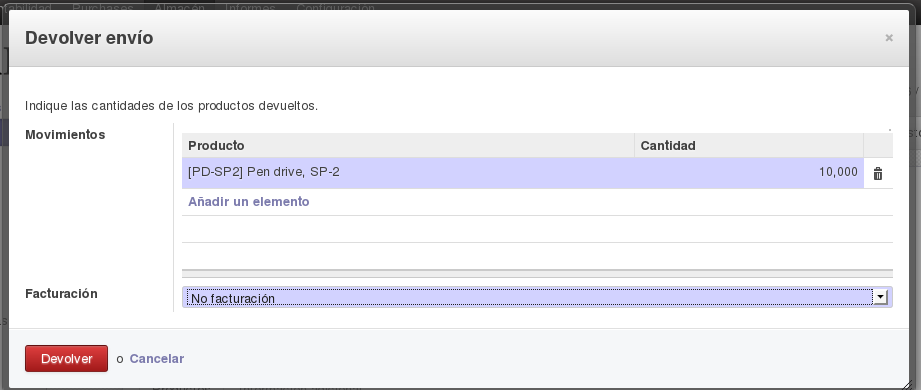
\includegraphics[width=\textwidth]{almacen/img/alb_entrada_dev.png}
\caption{Pestaña de devolución de productos}
\label{al:devolver}
\end{figure}




\vspace{0.5cm}
\subsection{Albaranes internos}
Los albaranes internos son utilizados en el caso de que su empresa tenga dos o más ubicaciones donde almacenar sus productos. En tales casos estos albaranes informan de cambios de ubicación entre las instalaciones de la empresa.


\vspace{0.5cm}
\subsection{Albaranes de salida}
Los albaranes de salida son los que hacen referencia a movimientos de productos desde un almacén propiedad de su empresa y los clientes. Se entienden como movimientos de salida de stock. La creación de los mismos se puede realizar de forma manual o de forma automática a través del modulo de ventas, generando una orden de venta.

En su concepción más básica, los albaranes de salida son y funcionan prácticamente igual que los albaranes de entrada. A continuación se va a recalcar principalmente las diferencias entre los albaranes de entrada y salida, pasando rápidamente por las secciones iguales y equivalentes en ambos tipos de albaranes.

\subsubsection{LISTADO DE ALBARANES DE SALIDA}
\label{almacen:envio}

\begin{figure}[H]
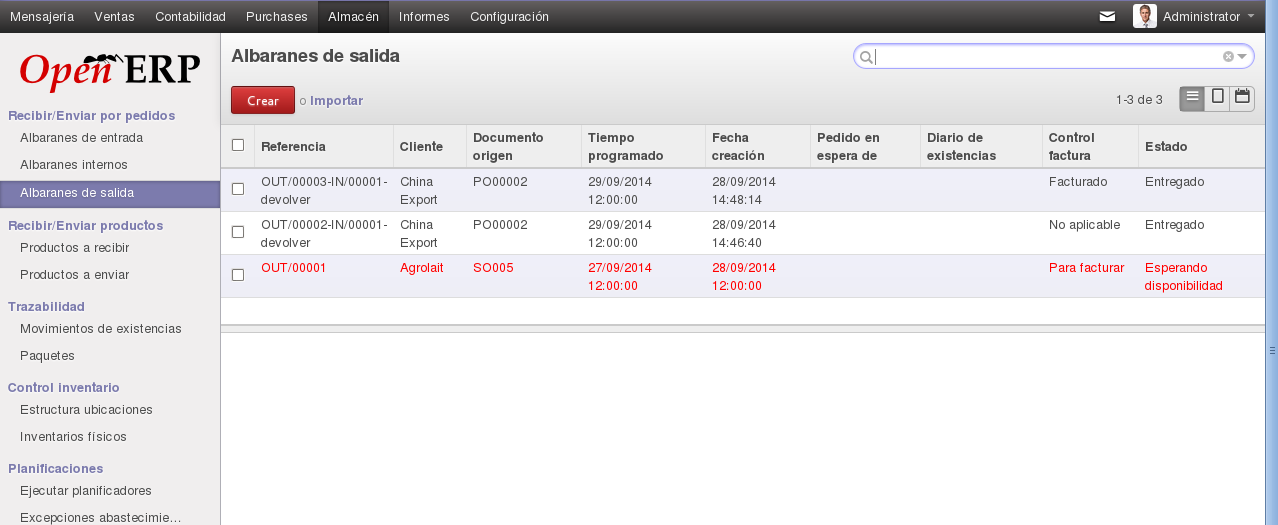
\includegraphics[width=\textwidth]{almacen/img/alb_salida.png}
\caption{Listado de albaranes de salida}
\label{al:listasalida}
\end{figure}

Los campos que se pueden observar en el listado de albaranes de salida son:

\begin{description}
  \item[Referencia] -- Referencia del albarán. Permite ver de un vistazo si es un albarán de salida normal o corresponde a alguna variación como a una devolución (pueden observarse dos albaranes de devolución en la figura \ref{al:listasalida}

  \item[Cliente] -- Cliente al que hace referencia el albarán y al que se le entregarán los productos.

  \item[Documento origen] -- Si el albarán ha sido generado automáticamente, este campo apunta al documento que dió lugar a su creación.

  \item[Tiempo programado] -- Tiempo calculado para servir los productos.

  \item[Fecha creación] -- Fecha en la que se ha creado el albarán

  \item[Pedido en espera de] -- Equivalente al mismo campo en los albaranes de entrada. Cuando se realiza un envío, puede realizarse por partes por las razones que sean (falta de stock, paquetes distintos) Cuando se realiza de tal manera, los productos del albarán que \textbf{no} son enviados, son incluidos en un nuevo albarán de salida, y ese albarán de salida tendrá este campo apuntando a ese albarán original con los materiales enviados.

  \item[Diario de existencias] -- Equivalente al mismo campo en los albaranes de salida.
 
  \item[Control factura] -- Al igual que en los albaranes de entrada, indica el estado de facturación, si procede, del albarán.

  \item[Estado] -- Indica el estado de los productos. Las posibilidades son:
    \begin{itemize}
    \item[*] \textbf{Borrador} -- Un albarán no confirmado y a la espera de ser confirmado o borrado.
    \item[*] \textbf{Esperando disponibilidad} -- Se encuentra a la espera de que los productos del albarán se encuentren disponibles.
    \item[*] \textbf{Lista para envío} -- Los productos están disponibles y es posible realizar el envío.
    \item[*] \textbf{Entregado} -- El albarán ha sido procesado integramente
    \end{itemize}
\end{description}


\vspace{0.5cm}
\subsubsection{ALBARAN DE SALIDA INDIVIDUAL}
Al igual que en los albaranes de entrada, hacer click sobre uno de los albaranes lo abrirá de manera individual mostrando los detalles del mismo.

\begin{figure}[H]
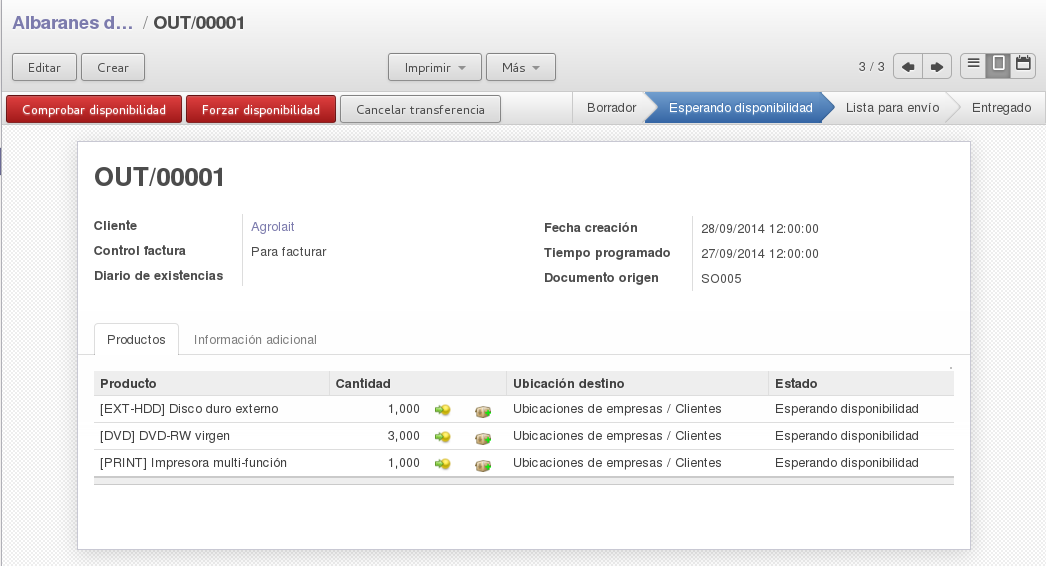
\includegraphics[width=\textwidth]{almacen/img/alb_salida_i.png}
\caption{Albarán de salida individual}
\label{al:salidaind}
\end{figure}

La parte superior del albarán es, al igual que en los albaranes de entrada, los mismos datos que se ven cuando se visualiza la lista de todos los albaranes de salida.

En la parte inferior están las mismas dos pestañas que en los albaranes de entrada con un funcionamiento idéntico. En este punto, la diferencia principal está en los posibles estados de cada producto. En este caso, los posibles estados son:

\begin{description}
  \item[Nuevo] -- Cuando se crea el albarán a mano y no ha sido confirmado aún.
  
  \item[Esperando otro movimiento] -- En caso de que el producto deba pasar por algún movimiento previo, el producto estára en este estado.

  \item[Esperando disponibilidad] -- En este caso, no hay suficiente disponibilidad del producto y queda a la espera de las variaciones del inventario hasta ser favorable.

  \item[Disponible] -- Existe stock del producto y puede ser enviado.

  \item[Reservado] -- Cuando se comprueba la disponibilidad de los productos mediante el botón homónimo en la parte superior del albarán, si existe suficiente stock del producto, lo reservará. Esto quiere decir que si se reserva en un albarán y aparece otro albarán después que requiere de los mismos productos, este segundo albarán verá el stock de productos como el total de los disponibles \textbf{menos} los reservados, evitando así que pedidos que no tienen material reservado se adelanten a otros que ya están siendo preparados.

En el caso de estar reservados y que por cualquier razón tengan que eliminar tal reserva, para ello se ha de hacer click sobre la línea del producto reservado y en la ventana emergente del producto (figura \ref{al:prodreser}, utilizar el botón \textbf{Cancelar disponibilidad}
\end{description}

\begin{figure}[H]
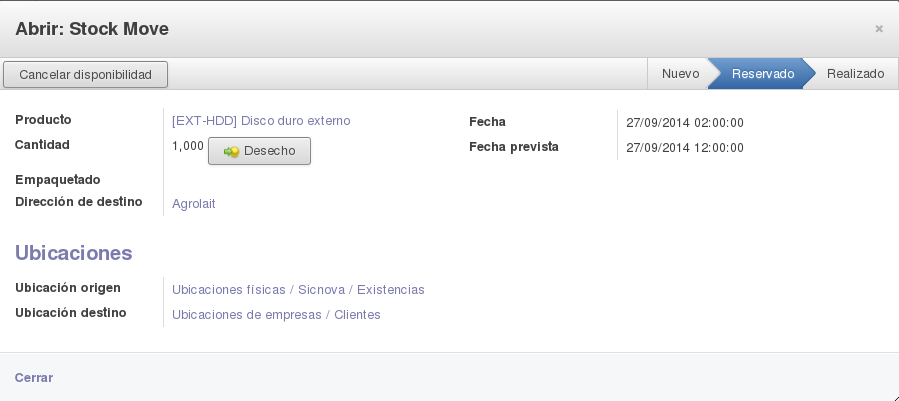
\includegraphics[width=\textwidth]{almacen/img/alb_salida_res.png}
\caption{Línea de un producto reservado para salida}
\label{al:prodreser}
\end{figure}

\vspace{0.5cm}
\subsubsection{ESTADOS DEL ALBARAN}

Los distintos estados y transiciones en los albaranes de salida son:

\begin{itemize}

  \item[$\star$] \textbf{Borrador} -- Albarán por confirmar, aún editable en todos sus campos. Este estado se da por defecto cuando se crea el albarán a través del botón \emph{Crear}.

    \begin{itemize}
      \item[--] \textbf{Confirmar} - Confirma el albarán y le permite pasar al estado \emph{Esperando disponibilidad}.
      \item[--] \textbf{Confirmar y enviar} - Confirma el albarán y da por enviados los productos. Da dos pasos en un solo click.
      \item[--] \textbf{Cancelar} - Cancela el albarán. Este paso no permite volver a ponerlo en estado de disponibilidad, hay que volver a crearlo tras cancelarlo.
    \end{itemize}



  \item[$\star$] \textbf{Esperando disponibilidad} -- Cuando el borrador es confirmado o cuando el albarán es creado automáticamente desde una orden de venta, pasará a este estado. En este punto pueden ocurrir dos cosas según si existe stock o no de alguno de los productos de las líneas.

    \begin{itemize}
    \item[--] \textbf{Existe stock de alguna línea de producto} - Si en algún producto hay stock, el albarán pasará al estado de \emph{Lista para el envío} en el caso de que la opción \emph{Método de entrega} de la pestaña \emph{Información adicional} tenga su valor en \emph{Parcial}. 

En caso de que su valor sea \emph{Todo junto}, sólo pasará al estado \emph{Lista para envío} cuando todos los productos estén disponibles.
      
    \item[--] \textbf{No existe stock de ningún producto} - En tal caso se permite la elección entre tres posibles pasos
      \begin{itemize}
      \item \textbf{Comprobar disponibilidad} Realiza un chequeo del stock de los productos. Si existe stock suficiente de alguna de las líneas de productos, realizará la reserva de los mismos y según el valor de \emph{Método de entrega} (explicado en el punto anterior) podrá pasar al estado de \emph{Lista para el envío}.

      \item \textbf{Forzar disponibilidad} Fuerza los productos como disponibles, situando el stock de los mismos en números negativos si es necesario y pasando el albarán al estado de \emph{Lista para el envío}.
      \end{itemize}
    \end{itemize}




  \item[$\star$] \textbf{Lista para envío} -- En este estado alguno o todos los productos se encuentran disponibles para el envío. En este punto sólo pueden realizarse dos acciones:

    \begin{itemize}
    \item[--] \textbf{Enviar} - Da por enviados los productos y realiza los cambios en el stock.
    \item[--] \textbf{Canclear} - Cancela el albarán y la transferencia de productos.
    \end{itemize}
\end{itemize}






\vspace{0.5cm}
\section{Recibir/Enviar Productos}
Los datos a los que se pueden acceder a través de las secciones de este menú son los mismos que en los submenús de la sección \emph{Recibir/Enviar por pedidos} con la salvedad de que se presentan de forma distinta.

En la sección anterior los datos se agrupaban por albaranes. Cada pedido/venta estaba relacionado con un albarán, el cual podía contener varías lineas de productos. En la actual sección se van a representar esas líneas de producto de forma independiente a los albaranes. Esto quiere decir que esta vista nos va a permitir ver los productos que están por entrar o por salir independientemente de sus albaranes y de los productos que puedan acompañarles en los mismos.

\subsection{Productos a recibir}
Las líneas representadas en esta sección corresponde a todos los productos contenidos en los albaranes de entrada.

\subsubsection{LISTADO DE PRODUCTOS A RECIBIR}

La vista por defecto al entrar en esta sección es la de la figura \ref{al:prodentrada}

\begin{figure}[H]
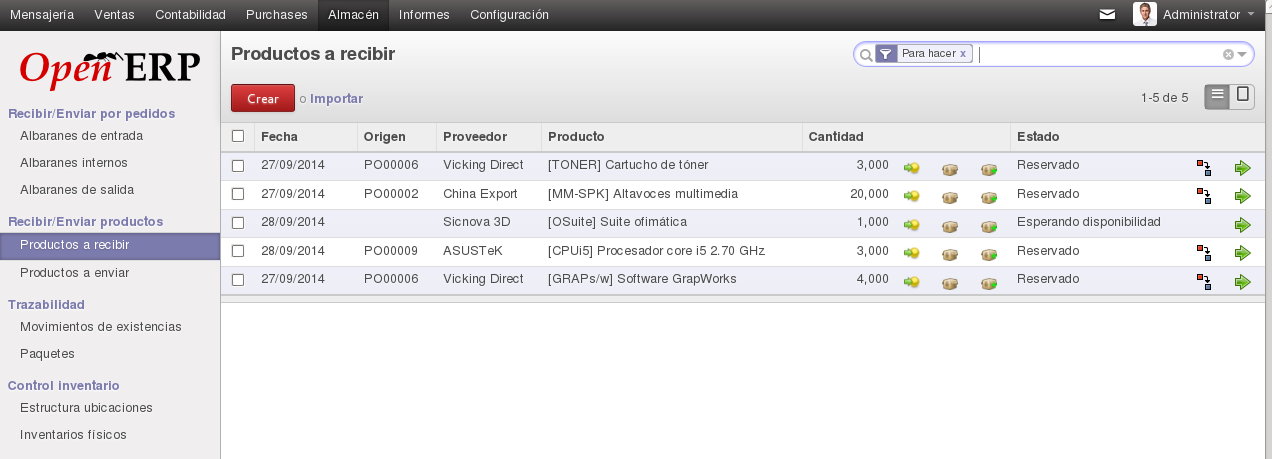
\includegraphics[width=\textwidth]{almacen/img/prod_entrada.png}
\caption{Lista de productos entrantes}
\label{al:prodentrada}
\end{figure}

Los campos disponibles son similares a los que se han visto en secciones anteriores relacionadas con los albaranes. En un repaso rápido y una explicación de algunos nuevos botones:

\begin{itemize}
  \item[*]\textbf{Fecha} -- Fecha de creación de la línea de pedido
  \item[*]\textbf{Origen} -- Documento que ha generado esta línea de pedido (si existe)
  \item[*]\textbf{Proveedor} -- Proveedor del producto
  \item[*]\textbf{Producto} -- Producto de la línea de pedido
  \item[*]\textbf{Cantidad} -- Cantidad de productos a recibir
  \item[*]\textbf{Botón de deshechar} -- No se utiliza desde los productos a recibir con la configuración actual. Es útil en caso de que en la recepción se utilizarán diversas ubicaciones físicas para la recepción del material y por el camino pudiera deshecharse parte del mismo.
  \item[*]\textbf{Botón de poner en el paquete actual} -- 
  \item[*]\textbf{Botón poner en un nuevo paquete} -- Realiza la división de los productos en varios paquetes.

Por defecto, cuando se piden X unidades de un producto, todas aparecen en la misma línea, representando esto que vienen en el mismo paquete. Mediante este botón se puede dividir el número de unidades de un producto en varias líneas, representando con esto que venían divididos en varios paquetes.

  \item[*]\textbf{Estado} -- Estado del pedido del producto. Más adelante se explica cuales son y como varían sus estados.

  \item[*]\textbf{Botón de procesado parcial} -- Cuando el producto se encuentra reservado, pueden procesarse parte de ese pedido para que forme parte del stock.

  \item[*]\textbf{Botón Realizado} -- Hacer click sobre este botón va a procesar esa línea del producto y va a dar por recibido ese producto incorporandolo al stock.

\end{itemize}


\subsubsection{LINEA DE PEDIDO INDIVIDUAL}

Al hacer click sobre uno de los elementos en el listado, se abrirá una visión individual del mismo como se ve en la figura \ref{al:prodentradai}

\begin{figure}[H]
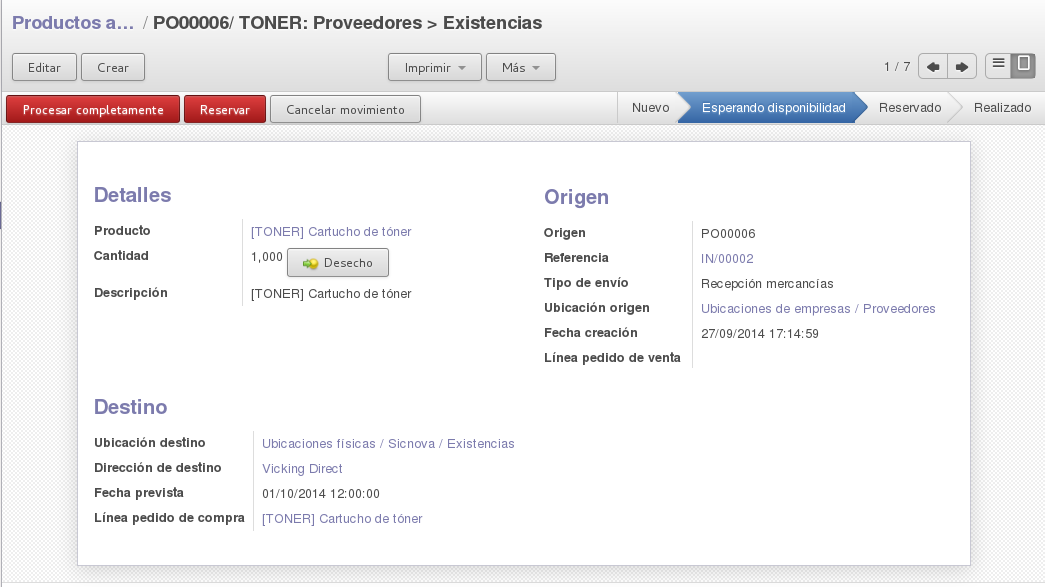
\includegraphics[width=\textwidth]{almacen/img/prod_entrada_i.png}
\caption{Linea de entrada individual}
\label{al:prodentradai}
\end{figure}

La visión individual engloba tres áreas con distinta información como son:

\begin{description}
  \item[Detalles] -- Que especifican los datos del producto de esa línea
    \begin{itemize}
    \item[$\star$] \textbf{Producto} - Nombre del producto que enlaza a la ficha del mismo
    \item[$\star$] \textbf{Cantidad} - Número de unidades del producto esperadas
    \item[$\star$] \textbf{Descripción} - Descripción del producto, insertada en la creación del mismo.
    \end{itemize}


  \item[Destino] -- Contiene la información relativa al lugar al que se va a realizar el movimiento de stock.
    \begin{itemize}
      \item[$\star$] \textbf{Ubicación destino} - Ubicación donde se contabilizará el stock
      \item[$\star$] \textbf{Dirección de destino} - Una desafortunada traducción. En este campo se indica la dirección y ficha de datos del proveedor.
      \item[$\star$] \textbf{Fecha prevista} - Fecha prevista de recepción de los productos.
      \item[$\star$] \textbf{Línea pedido de compra} - Nombre de la línea en el albarán.
    \end{itemize}

  \item[Origen] - Información relativa al origen de pedido, de la línea y del producto.
    \begin{itemize}
      \item[$\star$] \textbf{Origen} - Documento que origina el albarán en el que se encuentra la línea de producto.
      \item[$\star$] \textbf{Referencia} - Enlace al albarán que ha generado esta línea de producto
      \item[$\star$] \textbf{Tipo de envío} - Especifica que tipo de envío es, pudiendo elegirse entre \emph{Recepción de mercancías}, \emph{Envío de mercancías} e \emph{Interno}.
      Esta opción se rellena automáticamente según que tipo de albarán haya genereado esa línea de producto, sólo hay que rellenarla manualmente si se crean líneas de pedido individuales desde esta sección.
      \item[$\star$] \textbf{Ubicación origen} - Ubicación origen de la que aparecen estos productos.
      \item[$\star$] \textbf{Fecha creación} - Fecha en la que se ha creado la línea de pedido
      
    \end{itemize}
\end{description}

\vspace{.5cm}
Cuando la línea está creada correctamente y su estado es \textbf{Esperando disponibilidad} (ha pasado del su estado \emph{Nuevo} a \emph{Esperando disponibilidad} en el caso de crearla manualmente) pueden darse tres pasos con esa línea tal y como se ve en la figura \ref{al:prodentradai} anterior.
\begin{itemize}
\item[*] \textbf{Procesar completamente} - Da por recibidos los productos y pasa esta línea al estado de \textbf{Realizado}
\item[*] \textbf{Reservar} - Realiza la reserva en el stock de los productos, reflejandolo en las ubicaciones del stock e influyendo en lineas de pedidos posteriores, que tendrán en cuenta si hay más o menos stock según las reservas.
\item[*] \textbf{Cancelar movimientos} - Cancela estas líneas en el albarán correspondiente
\end{itemize}

\vspace{.5cm}
Cuando se realiza la reserva se pasa la línea al estado de \textbf{Reservado}. En este estado sólo caben dos opciones, tres si tenemos en cuenta que se pueden recibir productos parcialmente, los botones en ese estado se pueden ver en la figura \ref{al:prodentradares}

\begin{figure}[H]
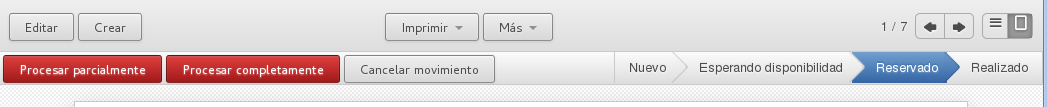
\includegraphics[width=\textwidth]{almacen/img/prod_salida_state.png}
\caption{Botones en el estado ``Reservado''}
\label{al:prodentradares}
\end{figure}

\begin{itemize}
\item[*] \textbf{Procesar parcialmente} - Mostrará un diálogo con el que se permite procesar sólo una parte de todo el pedido. Se usa cuando llega sólo una cantidad de productos que no es la esperada por la línea de producto.
\item[*] \textbf{Procesar completamente} - Da por recibido todos los productos y pasa la línea al estado de \textbf{Realizado}
\item[*] \textbf{Cancelar movimiento} - Cancela la línea de pedido.
\end{itemize}

\subsection{Productos a enviar}
En esta parte, el funcionamiento y la presentación de la información de las líneas es exactamente igual que en la anterior. 

La diferencia principal es que, en este caso, las líneas que se muestran son las de los productos de los \textbf{albaranes de salida}. Esto quiere decir que es una especie de sección espejo, se maneja y fucniona igual que \emph{Productos a recibir} con la salvedad de que hay que tener en cuenta que los movimientos de stock van \emph{al revés}.

Si en la sección anterior se podían ver y manipular los productos que venían de los proveedores al stock de nuestra empresa, en esta sección hay que tener claro que se está trabajando con movimientos que van desde nuestro stock hacia los clientes.






\section{Trazabilidad}

\subsection{Movimientos de existencias}
Esta sección muestra \textbf{todos} los movimientos de productos línea a línea, tanto los envíados como los recibidos. Da una visión global de todos
los movimientos para busquedas avanzadas.

También se incluyen aquí movimientos que no están relacionados directamente con los albaranes como pueden ser las ordenes de abastecimiento creadas
por las cantidades mínimas de stock como se verá más adelante.

\begin{figure}[H]
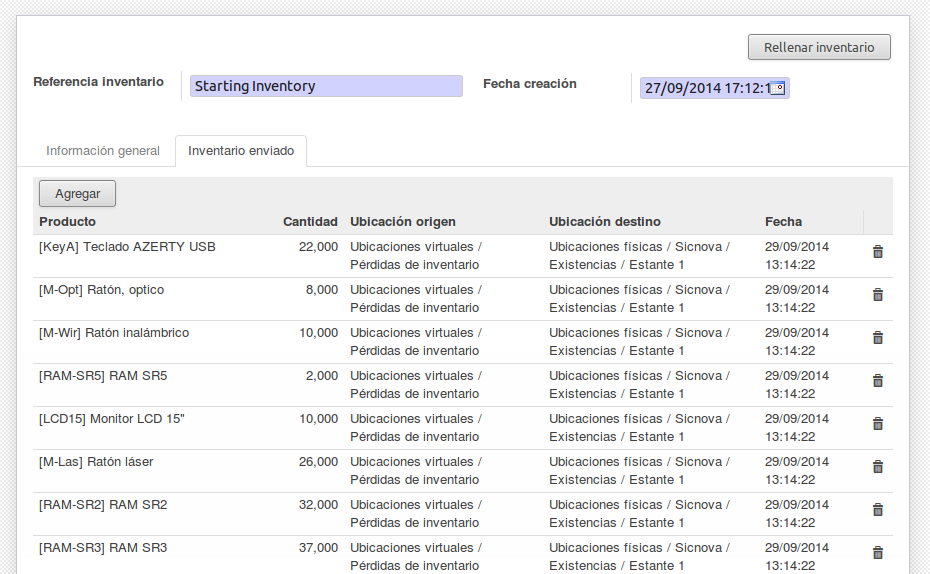
\includegraphics[width=\textwidth]{almacen/img/tra_mov.png}
\caption{Pantalla de movimiento de existencias}
\label{al:movex}
\end{figure}

%\subsection{Paquetes}






\section{Control Inventario}

A través de esta sección se llevará el inventario y se podrá controlar de forma semiautomática los inventarios y movimientos, así como las posibles perdidas de inventario y otros detalles relativos al stock.

\subsection{Estructura ubicaciones}
Aquí se va a presentar un menú desplegable y una zona para desplegar información en forma de árbol.

El desplegable permite elegir entre los tres tipos de ubicaciones posibles:
\begin{description}
  \item[Ubicaciones físicas] -- Ubicaciones que representan un espacio físico concreto como puede ser las zonas de almacenaje de las empresas. Se representa en la figura \ref{ub:fisicas}
\begin{figure}[H]
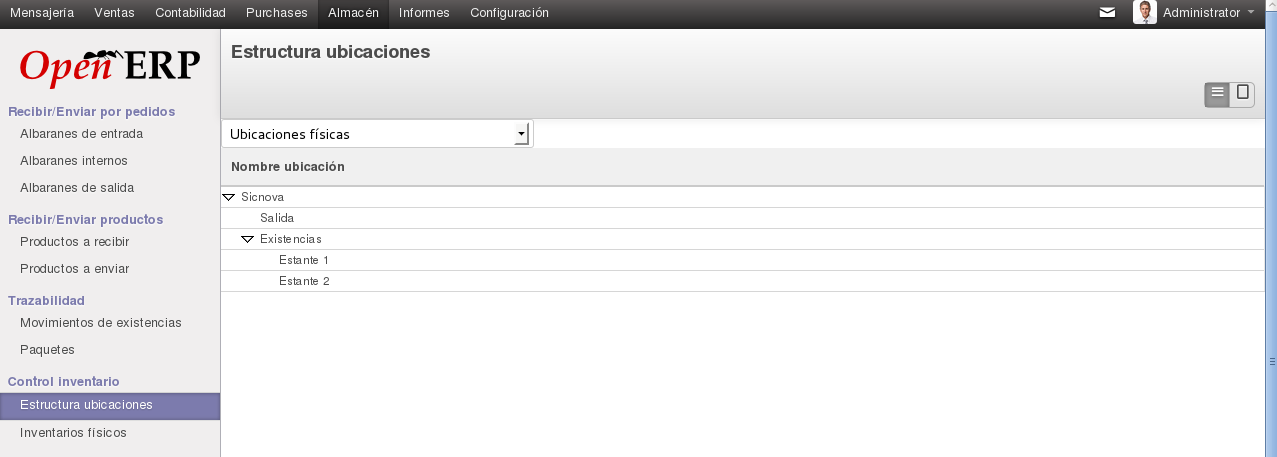
\includegraphics[width=\textwidth]{almacen/img/ubi_fisica.png}
\caption{Ejemplo de ubicaciones físicas}
\label{ub:fisicas}
\end{figure}

  \item[Ubicaciones de empresas] -- Ubicaciones relativas a clientes, proveedores y envíos internos.
  \item[Ubicaciones virtuales] -- Este tipo de ubicaciones es también importante ya que entre ellas se puede encontrar la ubicación de \emph{Pérdidas de inventario} que puede ser crítica para el análisis del stock. Puede verse en la figura \ref{ub:virtuales}
\end{description}


\begin{figure}[H]
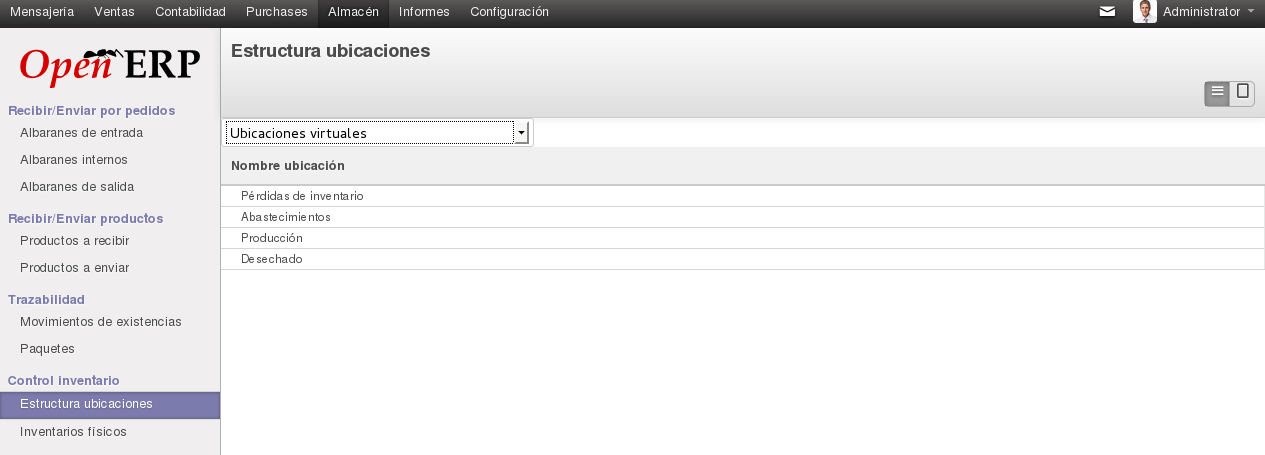
\includegraphics[width=\textwidth]{almacen/img/ubi_virtual.png}
\caption{Ubicaciones virtuales por defecto}
\label{ub:virtuales}
\end{figure}


Hacer click sobre cualquiera de estas ubicaciones abrirá un diálogo que llevará a una visualización del inventario en la ubicación marcada. Este dialogo permitirá elegir como mostrar el inventario mediante la elección del \emph{Tipo de análisis}. El menú es el que se puede ver en la figura \ref{ub:inventariomenu}. Las opciones de esta elección son:


\begin{itemize}
  \item \textbf{Analizar inventorio actual} - Muestra el inventorio teniendo en cuenta \emph{todos} los movimientos de stock
                                            en la base de datos
  \item \textbf{Analizar periodo} - Permite elegir la fecha inicial y final para el análisis del inventario. Es lo más
                                   práctico para análisis más minuciosos.
\end{itemize}

\begin{figure}[H]
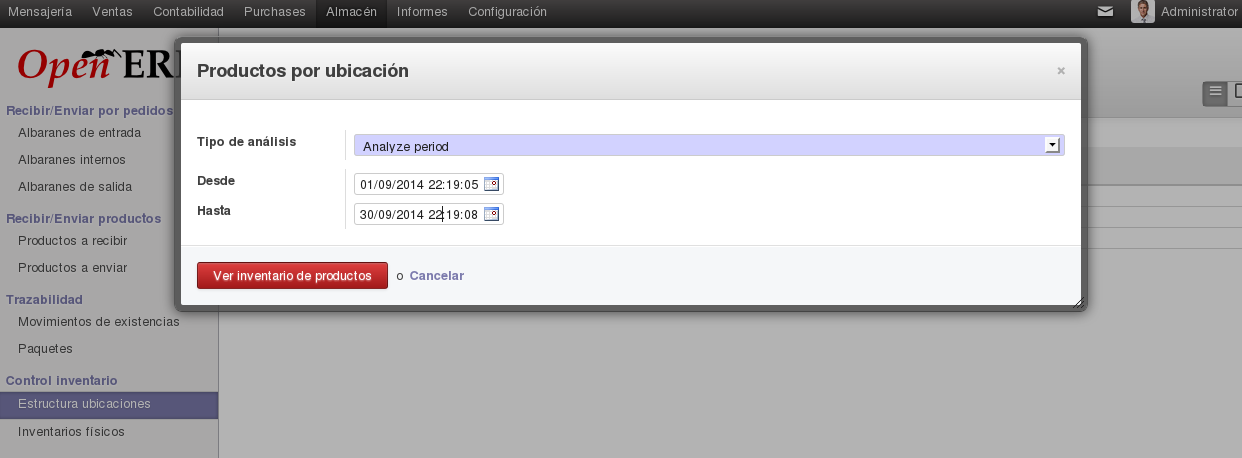
\includegraphics[width=\textwidth]{almacen/img/ubi_invent_menu.png}
\caption{Menú de análisis de inventario}
\label{ub:inventariomenu}
\end{figure}


El inventario mostrado contiene la información de los productos existentes en el mismo y una previsión de los que habrá cuando se vayan aprobando los distintos albaranes y transacciones de productos. Un ejemplo de este inventario se puede ver en la figura \ref{ub:inventarioej} con una descripción de los campos tras la figura.

\begin{figure}[H]
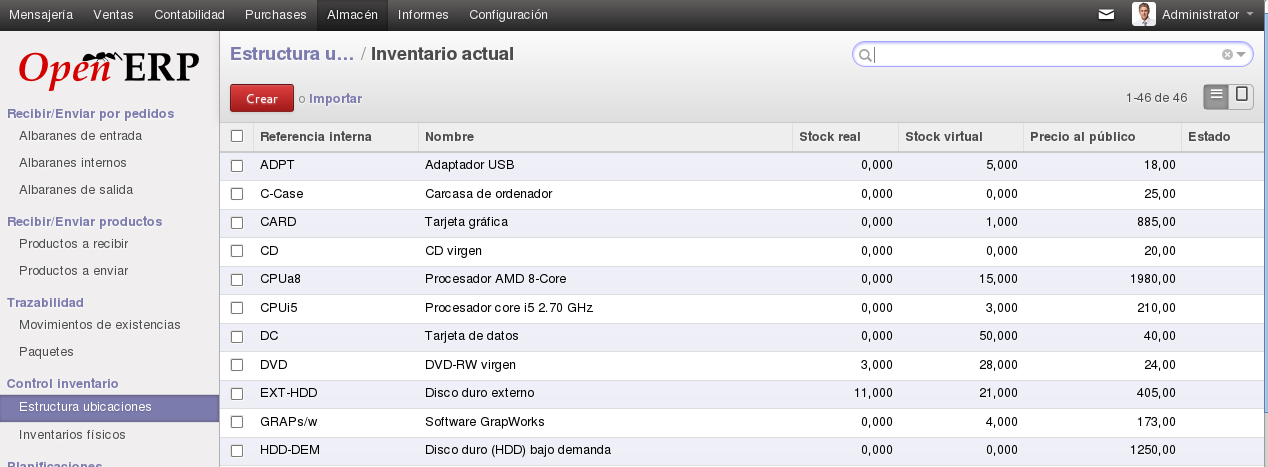
\includegraphics[width=\textwidth]{almacen/img/ubi_inventario.png}
\caption{Inventario físico de ejemplo}
\label{ub:inventarioej}
\end{figure}


\begin{description}
  \item[Referencia interna] -- Referencia del producto. Especificada en la ficha del mismo.
  \item[Nombre] -- Nombre del producto.
  \item[Stock real] -- Stock existente en el momento actual.
  \item[Stock virtual] -- Stock que pasará a ser real en cuanto se ejecuten las transacciones de productos pendientes. Este stock se calcula mediante
                          el stock real - stock saliente + stock entrante, siendo estos dos últimos (entrante y saliente) las operaciones pendientes
  \item[Precio al público] -- Precio del producto al público. Especificado en la ficha del producto.
\end{description}


\subsection{Inventarios físicos}
Los inventarios físicos, como su nombre indica, hacen referencia a los inventarios, los recuentos de material disonibles físicamente. En esta zona del
programa es a través de la cual se informará de los recuentos de material y se mezclará con la información de las transacciones de productos realizadas
para finalmente poder obtener un informe detallado de lo que se tiene y de lo que se debería tener y, por ende, fallos en transacciones, en recuentos, 
existencia de material perdido...

\subsubsection{Listado de inventarios}
Al entrar en esta opción, la primera visión de los inventarios es un listado de los mismos (figura \ref{ub:inventariolista}). Los datos visibles de los mismos serán:

\begin{itemize}
  \item \textbf{Referencia inventario} -- Referencia del inventario que se le da a la hora de crearlo.
  \item \textbf{Fecha de creación} -- Fecha en la que se ha creado el inventario.
  \item \textbf{Estado} -- Estado del inventario. El mismo puede tener tres estados:
    \begin{itemize}
      \item[$\star$] \textbf{Borrador} - Se han hecho los recuentos apropiados pero no se ha confirmado. En este estado, la información contenida
                                         en el inventario no modifica la información de stock de los productos en la base de datos.
      \item[$\star$] \textbf{Confirmado} - El paso siguiente tras el borrador. En este estado, la información de recuentos se refleja en la base de
                                           datos. En este caso, los recuentos influyen sólo en el stock virtual.
      \item[$\star$] \textbf{Realizado} - Una vez confirmado y comprobados todos los pasos, se valida el inventario. Es en este momento en el que
                                          los calculos pasan a ser efectivos y se modifica el stock real en la base de datos.
    \end{itemize}
\end{itemize}

\begin{figure}[H]
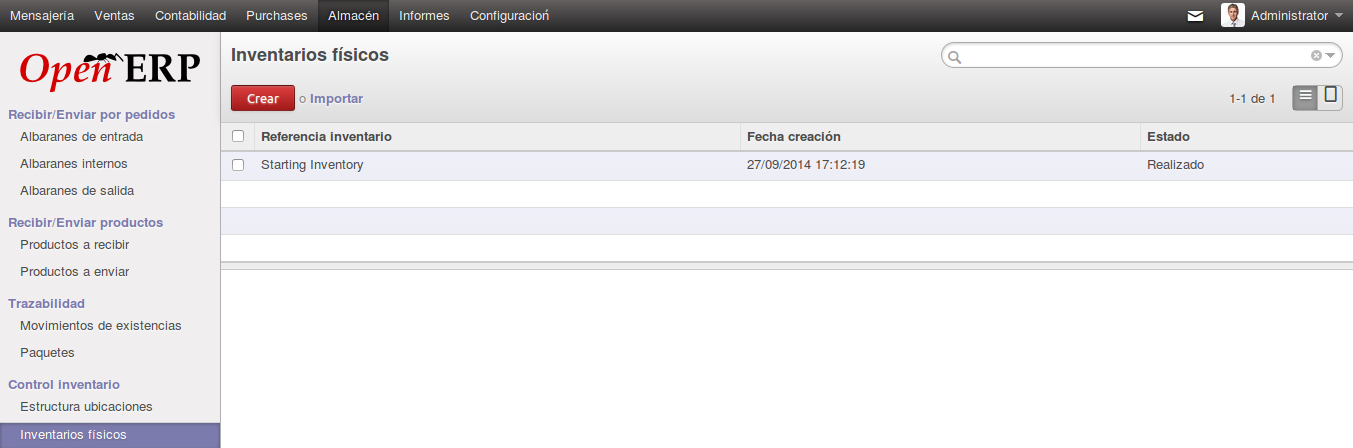
\includegraphics[width=\textwidth]{almacen/img/inv_lista.png}
\caption{Listado de inventarios}
\label{ub:inventariolista}
\end{figure}	

Haciendo click sobre uno de los inventarios o pulsando el botón de crear, se procede al inventario seleccionado o a crear un nuevo inventario como se
ve en la figura \ref{ub:inventarioindividual}. Los datos a rellenar son los mismos que los que se han visto en el listado de inventarios aparte de dos
pestañas que se rellenan con los datos del inventario.

En la pestaña de \textbf{información general} (también se puede ver en la figura \ref{ub:inventarioindividual}) los datos a rellenar son:

\begin{itemize}
  \item \textbf{Ubicación} -- Ubicación física en la que se encuentra el material recontado.
  \item \textbf{Producto} -- Producto que se está inventariando.
  \item \textbf{Cantidad} -- Cantidad de producto a inventariar.
\end{itemize}

\begin{figure}[H]
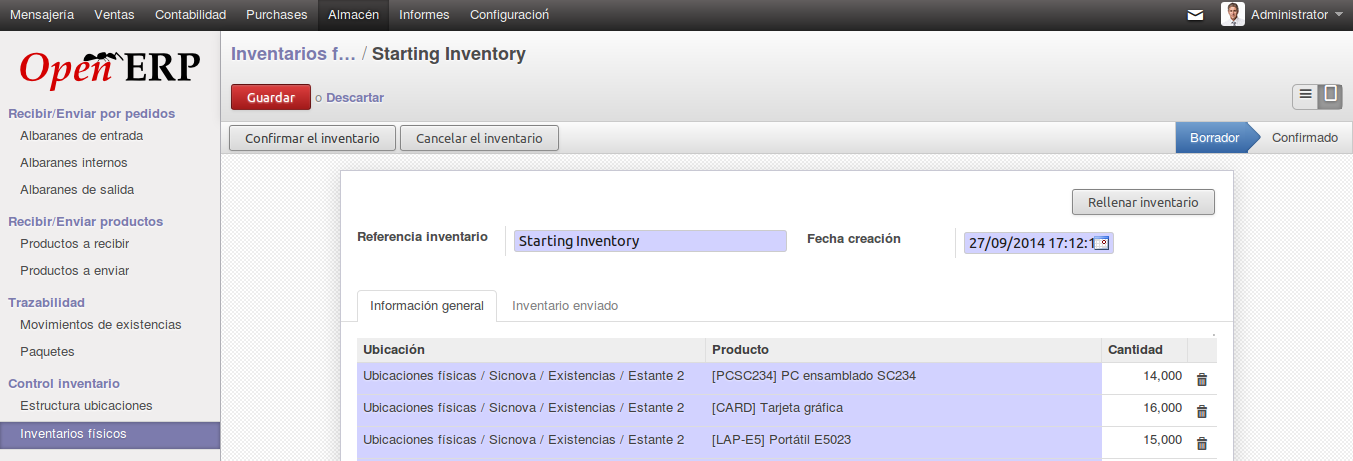
\includegraphics[width=\textwidth]{almacen/img/inv_ind.png}
\caption{Edición de inventario}
\label{ub:inventarioindividual}
\end{figure}	

El botón \emph{Rellenar inventario} ayuda a importar el inventario actual. Abre una ventana emergente (figura \ref{ub:inventarioimportar}) que,
una vez seleccionada la ubicación, importa todos los productos contenidos en esa ubicación y su número actual en la lista de productos del inventario
que se está creando/rellenando. La importación admite dos opciones que se presentan como checkboxes:

\begin{itemize}
  \item \textbf{Incluir hijos} -- Incluye, en la importación, todos los productos que existan también en las ubicaciones hijas de la ubicación
                                  seleccionada.
  \item \textbf{Inicializar a cero} -- Pone a 0 la cantidad de productos en la lista del inventario que se está creando/editando.
\end{itemize}

\begin{figure}[H]
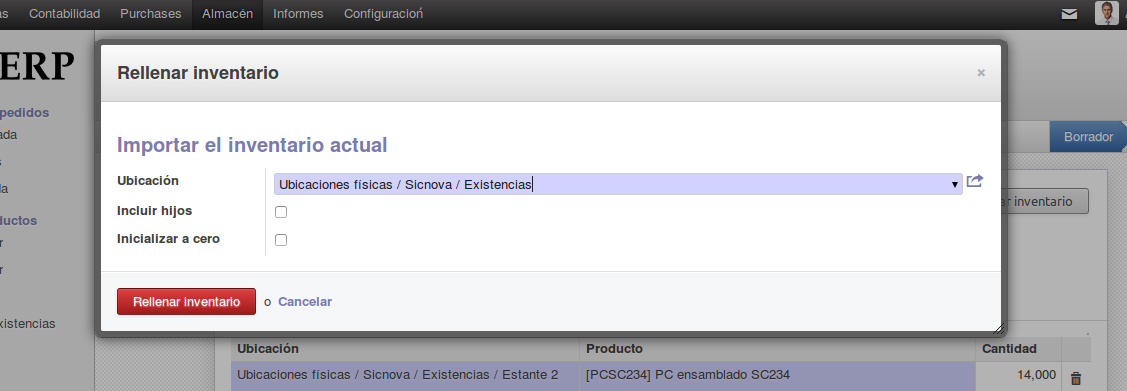
\includegraphics[width=\textwidth]{almacen/img/inv_imp.png}
\caption{Importación del inventario}
\label{ub:inventarioimportar}
\end{figure}


La otra pestaña disponible es la de \textbf{Inventario enviado}. En esta pestaña se rellena con la información de las transacciones de productos
ya realizadas, es decir, con la información de los albaranes de entrada salida. Mediante el botón \emph{Agregar}, que se puede apreciar en la
figura \ref{ub:inventarioenviado}, se despliega un menú que permite seleccionar que transacciones se van a incluir en esta pestaña. Lo habitual es
incluirlas todas.

\begin{figure}[H]
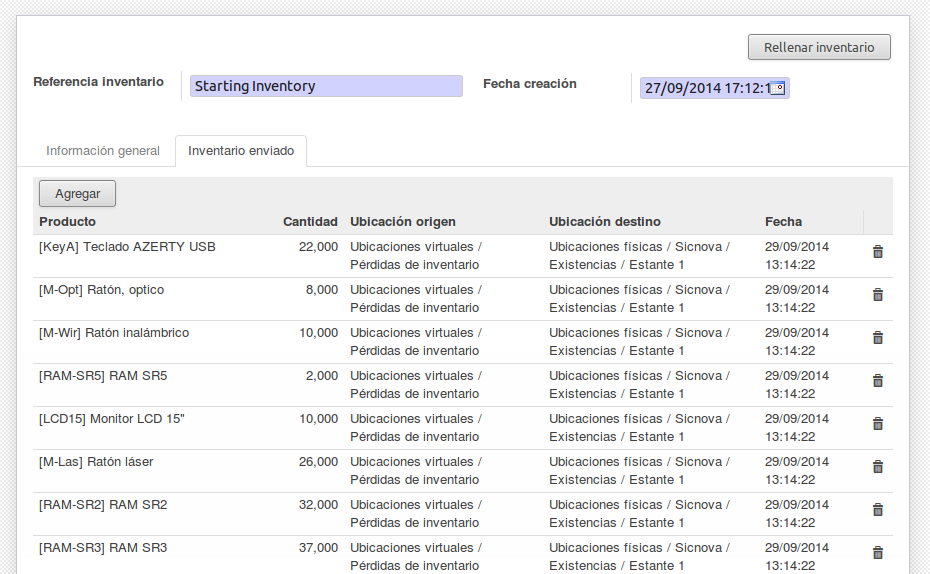
\includegraphics[width=\textwidth]{almacen/img/inv_env.png}
\caption{Importación del inventario}
\label{ub:inventarioenviado}
\end{figure}

Mediante el inventario físico se está indicando al software cuál es la cantidad de productos disponibles, y será la utilizada en el stock.
Con el inventario enviado el software calcula cuál sería la cantidad de productos disponibles en función del inventario existente anteriormente.
Si los calculos no corresponden, el software presentará esa diferencia en la ubicación \emph{Perdidas de inventario} como señal de la necesidad
de revisar las transacciones del producto correspondiente.




\section{Planificaciones}
Con OpenERP se pueden realizar planificaciones de aprovisionamiento. Se pueden definir unas reglas para poder tener siempre entre un mínimo y
un máximo de stock de productos. Esta configuración se realiza de manera individual para cada producto.

\subsection{Ejecutar planificadores}
\label{planificadores}
Esta opción disparará todas las reglas de planificación de stock. En caso de que haya productos que no cumplas con las reglas del mínimo
establecido, generará automáticamente ordenes de abastecimiento que podrán ser comprobadas a mano y, a su vez, generará presupuestos de compra
en el módulo de compras con los artículos que no cumplan los mínimos.

El encargado de compras podrá ver aparecer los nuevos presupuestos de compra con una referencia a la orden de abastecimiento, sabiendo así que
la compra a realizar aparece para cumplir las mínimas cantidades en el stock.

\begin{figure}[H]
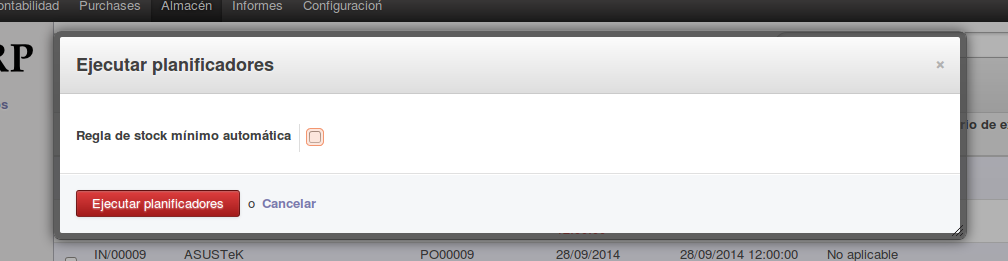
\includegraphics[width=\textwidth]{almacen/img/inv_plan.png}
\caption{Ejecución de planificadores}
\label{ub:inventarioplan}
\end{figure}

La figura \ref{ub:inventarioplan} muestra la ventana flotante que aparece tras seleccionar la opción de ejecución de los planificadores. Seleccionar
la opción \emph{Regla de stock mínima automática} hará que \textbf{todos} los productos que tengan un stock virtual menor que 0 ejecuten una orden
de abastecimiento para dejar este stock virtual a 0. No es recomendable utilizar esta opción puesto que puede generar pedidos indeseados.

\subsection{Excepciones abastecimiento}
Si tras ejecutar las planificaciones existiese algún problema con el stock, aparecerá aquí marcado en rojo. En cualquier otro caso se podrán ver como
en la figura \ref{ub:inventarioerr}

\begin{figure}[H]
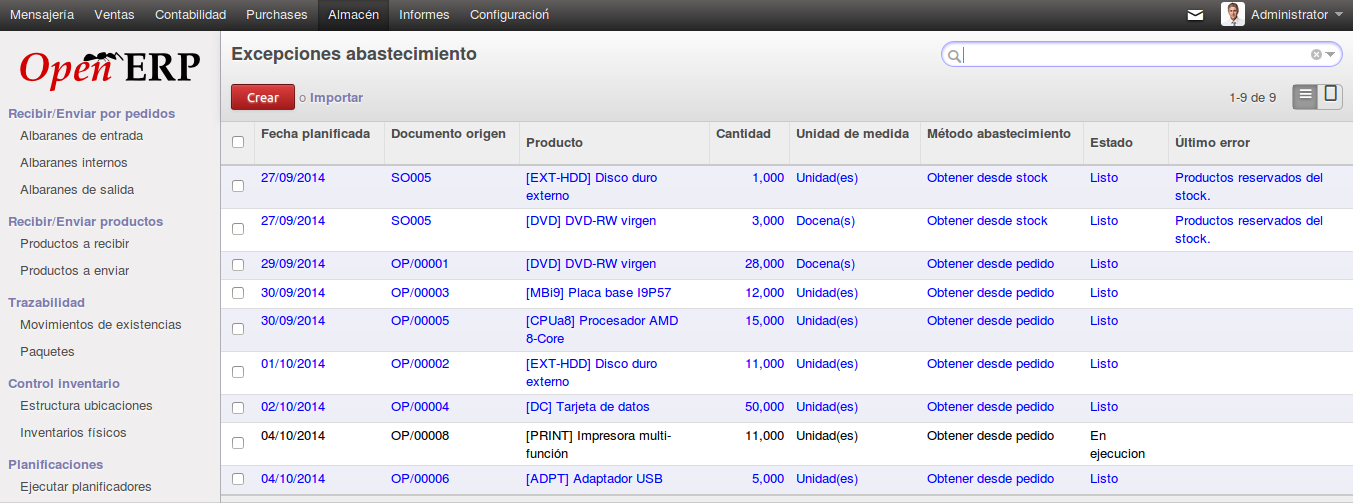
\includegraphics[width=\textwidth]{almacen/img/inv_error.png}
\caption{Ejecución de planificadores}
\label{ub:inventarioerr}
\end{figure}

Los campos que se pueden apreciar en esta sección son:

\begin{itemize}
  \item \textbf{Fecha planificada} -- Fecha calculada en la que se producirá el abastecimiento
  \item \textbf{Documento orgien} -- Referencia al documento que ha creado la orden de abastecimiento
  \item \textbf{Product} -- Producto al que hace referencia la orden
  \item \textbf{Cantidad} -- Cantidad de producto a pedir
  \item \textbf{Unidad de medida} -- Unidad de medida de las cantidades del producto
  \item \textbf{Método de abastecimiento} -- Indica de donde se obtiene el abastecimiento de este producto. Los que se puede encontrar es:
    \begin{itemize}
       \item[$\star$] \textbf{Obtener desde stock} - Las ordenes de venta, por ejemplo, pueden requerir de productos que estén en stock, en tal
                                                    caso, el abastecimiento del producto para el pedido se realiza desde el stock
       \item[$\star$] \textbf{Obtener desde pedido} - Algunos productos pueden configurarse para que cuando sean requeridos, se genere una orden 
                                                    de pedido. Cuando se ejecutan los planificadores, al encontrar productos que no cumplen los
                                                    mínimos también crea presupuestos para pedidos a proveedores, siendo pues este tipo de
                                                    abastecimiento también.
    \end{itemize}
  \item \textbf{Estado} -- Estado de la orden de excepción
    \begin{itemize}
      \item[$\star$] \textbf{Borrador} - Estado por defecto al crear la orden de abastecimiento. Si son creadas automáticamente, pasarán a alguno
                                         de los estados siguientes
      \item[$\star$] \textbf{Confirmado} - Estado alcanzado cuando se confirma el abastecimiento
      \item[$\star$] \textbf{En ejecución} - Estado tras la confirmación
      \item[$\star$] \textbf{Excepción} - Este estado se alcanza en el caso de que ocurra algún error. La orden aparecerá en rojo.
      \item[$\star$] \textbf{Listo} - Tras eliminar la excepción la orden pasará a este estado.
      \item[$\star$] \textbf{Esperando} - La orden está a la espera de que alguna otra sea atendida. Este estado puede aparecer si se usan opciones
                                          de manufacturación
    \end{itemize}
  \item \textbf{Último error} -- Especifica que es lo que ha provocado la excepción de abastecimiento de manera que permita buscar una solución.
\end{itemize}



\section{Configuración del módulo}
Con los subsiguientes menús se puede realizar una configuración más personalizada de algunos de los parámetros del módulo de almacén.

\subsection{Reglas de reabastecimiento}
\label{alm:reabastecimiento}

A través de esta opción se presentará un menú que permitirá la inserción de reglas de reabastecimiento. Tales reglas consisten en la inserción de una cantidad mínima y máxima de cada elemento del almacén. En el momento en el que el \emph{stock virtual} se situa \textbf{por debajo} de un nivel mínimo establecido, se generará automáticamente un abastecimiento para que el stock del producto sea el especificado a través de la cantidad máxima.

Puede crearse tantas reglas de reabastecimiento como sean necesarias, en la figura \ref{alm:lista-reabast}.

\figura{almacen/img/rea_list.png}
{Listado de reglas de reabastecimiento}
{alm:lista-reabast}

A través de la vista de listado de las reglas de reabastecimiento se puede ver rápidamente que productos se encuentran con reglas de reabastecimiento y las cantidades mínimas y máximas de los mismos.

La ficha individual sobre la información se aprecia en la siguiente figura (\ref{alm:rea-individual})

\figura{almacen/img/rea_individual.png}
{Ficha individual de producto}
{alm:rea-individual}

El campo \textbf{Nombre} será el identificador único de esta orden. Será lo que permitirá organizar los pedidos, habitualmente se utiliza un prefijo con una numeración como se ve en el ejemplo. 

En el campo \textbf{producto} se introducirá el producto para el que se está creando y para el que se aplicará la regla de reabastecimiento.

Los campos bajo el texto \textbf{Reglas} indican la \textbf{cantidad mínima} -- que indica cual es el límite para el stock virtual a partir del que se realizará una orden de pedido --, la \textbf{cantidad máxima} que será la cantidad a alcanzar cuando se realice el proceso de reabastecimiento y el \textbf{Múltiplo de la cantidad}, que será a que cifra se redondeará el pedido en el caso de que se utilicen cifras con decimales para el producto.

En el área de \textbf{Varios} se podrá acceder, mediante un enlace, al \textbf{Último abastecimiento} realizado y podrá activarse o desactivarse la orden de reabastecimiento con la casilla \textbf{Activo}. La utilidad de desactivar las ordenes son validas para evitar que se realicen los pedidos del producto sin borrar la orden para, en caso de necesidad, vovler a reactivarla en cualquier momento sin haber llegado a perderla.

El listado que se encuentra bajo el texto \textbf{Órdenes de abastecimiento a procesar} muestra las ordenes disponibles en el sistema que están listas para ser procesadas -- como su propio nombre indica --, relacionados con el producto y su reabastecimiento.

Hay que recordar que para generar estas ordenes de pedido a través de las ordenes de reabastecimiento, hay que hacer uso periodico de la opción \textbf{Ejecutar planificadores} del menú del módulo de almacén, eligiendo la opción \textbf{Regla de stock mínima automática}, tal como se indica en la sección \ref{planificadores}.



%%%
%%%  Anexos
%%%
\part*{Anexos}
\addcontentsline{toc}{part}{Anexos}

%%%
%%% Información sobre el documento
%%%
\addcontentsline{toc}{chapter}{Sobre este documento}
\chapter*{Sobre este documento}

El documento que tiene en sus manos ha sido creado por Gabriel Franco, componente de la Filé Aesir (\url{http://fileaesir.com}) con la 
finalidad de poder documentar el software aquí descrito OpenERP / Odoo debido, principalmente, a la falta de documentación en castellano
sobre el mismo. Esperamos que, a medida que avancemos en versiones, el contenido pase de unas simples instrucciones para el uso de
las funciones más básicas a un completo manual que alcance, esperamos en cierta medida, elementos como incluso el desarrollo de módulos
y conceptos más profundos que los del simple usuario.

Lo publicamos bajo licencia GNU Free Documentation License, Version 1.3, para compartirlo con la comunidad y dar la posibilidad a todos
aquellos que lo deseen, de compartir y colaborar en este documento/guía líbremente.

Para cualquier consulta, duda o sugerencia se puede contactar con nosotros a través de la cuenta en Github relacionada con el repositorio
donde se encuentra este documento y su fuente \url{https://github.com/Gabriel-fm/oerp-manual} o a través del correo \href{mailto:file@fileaesir.com}{file@fileaesir.com}

El enlace desde el que podrá descargar y obtener este documento (y sus fuentes en formato TeX) se encuentra disponible en \url{https://github.com/Gabriel-fm/oerp-manual}


%%%
%%% Historial de cambios
%%%
\addcontentsline{toc}{chapter}{Historial de cambios}
\chapter*{Historial de cambios}
\begin{description}
  \item[v0.2] Incluído el módulo de Ventas
  \item[v0.3] Inlcuido el módulo de Contabilidad
  \item[v0.3.5] Terminado el módulo de Contabilidad
  \item[v0.4] Añadidas ordenes de reabastecimiento en almacén y capítulo sobre los productos
  \item[v0.5] Reglas de stock mínimas explicadas
\end{description}



%%%
%%%  Texto Licencia GFDL
%%%
\chapter*{\rlap{GNU Free Documentation License}}
%%\phantomsection  % so hyperref creates bookmarks
%\addcontentsline{toc}{chapter}{Apendices}
%\chapter{Apendices}
\addcontentsline{toc}{chapter}{GNU Free Documentation License}
%\chapter*{\rlap{GNU Free Documentation License}}
%\label{label_fdl}

 \begin{center}

       Version 1.3, 3 November 2008


 Copyright \copyright{} 2000, 2001, 2002, 2007, 2008  Free Software Foundation, Inc.
 
 \bigskip
 
     \texttt{<http://fsf.org/>}
  
 \bigskip
 
 Everyone is permitted to copy and distribute verbatim copies
 of this license document, but changing it is not allowed.
\end{center}


\begin{center}
{\bf\large Preamble}
\end{center}

The purpose of this License is to make a manual, textbook, or other
functional and useful document ``free'' in the sense of freedom: to
assure everyone the effective freedom to copy and redistribute it,
with or without modifying it, either commercially or noncommercially.
Secondarily, this License preserves for the author and publisher a way
to get credit for their work, while not being considered responsible
for modifications made by others.

This License is a kind of ``copyleft'', which means that derivative
works of the document must themselves be free in the same sense.  It
complements the GNU General Public License, which is a copyleft
license designed for free software.

We have designed this License in order to use it for manuals for free
software, because free software needs free documentation: a free
program should come with manuals providing the same freedoms that the
software does.  But this License is not limited to software manuals;
it can be used for any textual work, regardless of subject matter or
whether it is published as a printed book.  We recommend this License
principally for works whose purpose is instruction or reference.


\begin{center}
{\Large\bf 1. APPLICABILITY AND DEFINITIONS\par}
%%\phantomsection
%\addcontentsline{toc}{section}{1. APPLICABILITY AND DEFINITIONS}
\end{center}

This License applies to any manual or other work, in any medium, that
contains a notice placed by the copyright holder saying it can be
distributed under the terms of this License.  Such a notice grants a
world-wide, royalty-free license, unlimited in duration, to use that
work under the conditions stated herein.  The ``\textbf{Document}'', below,
refers to any such manual or work.  Any member of the public is a
licensee, and is addressed as ``\textbf{you}''.  You accept the license if you
copy, modify or distribute the work in a way requiring permission
under copyright law.

A ``\textbf{Modified Version}'' of the Document means any work containing the
Document or a portion of it, either copied verbatim, or with
modifications and/or translated into another language.

A ``\textbf{Secondary Section}'' is a named appendix or a front-matter section of
the Document that deals exclusively with the relationship of the
publishers or authors of the Document to the Document's overall subject
(or to related matters) and contains nothing that could fall directly
within that overall subject.  (Thus, if the Document is in part a
textbook of mathematics, a Secondary Section may not explain any
mathematics.)  The relationship could be a matter of historical
connection with the subject or with related matters, or of legal,
commercial, philosophical, ethical or political position regarding
them.

The ``\textbf{Invariant Sections}'' are certain Secondary Sections whose titles
are designated, as being those of Invariant Sections, in the notice
that says that the Document is released under this License.  If a
section does not fit the above definition of Secondary then it is not
allowed to be designated as Invariant.  The Document may contain zero
Invariant Sections.  If the Document does not identify any Invariant
Sections then there are none.

The ``\textbf{Cover Texts}'' are certain short passages of text that are listed,
as Front-Cover Texts or Back-Cover Texts, in the notice that says that
the Document is released under this License.  A Front-Cover Text may
be at most 5 words, and a Back-Cover Text may be at most 25 words.

A ``\textbf{Transparent}'' copy of the Document means a machine-readable copy,
represented in a format whose specification is available to the
general public, that is suitable for revising the document
straightforwardly with generic text editors or (for images composed of
pixels) generic paint programs or (for drawings) some widely available
drawing editor, and that is suitable for input to text formatters or
for automatic translation to a variety of formats suitable for input
to text formatters.  A copy made in an otherwise Transparent file
format whose markup, or absence of markup, has been arranged to thwart
or discourage subsequent modification by readers is not Transparent.
An image format is not Transparent if used for any substantial amount
of text.  A copy that is not ``Transparent'' is called ``\textbf{Opaque}''.

Examples of suitable formats for Transparent copies include plain
ASCII without markup, Texinfo input format, LaTeX input format, SGML
or XML using a publicly available DTD, and standard-conforming simple
HTML, PostScript or PDF designed for human modification.  Examples of
transparent image formats include PNG, XCF and JPG.  Opaque formats
include proprietary formats that can be read and edited only by
proprietary word processors, SGML or XML for which the DTD and/or
processing tools are not generally available, and the
machine-generated HTML, PostScript or PDF produced by some word
processors for output purposes only.

The ``\textbf{Title Page}'' means, for a printed book, the title page itself,
plus such following pages as are needed to hold, legibly, the material
this License requires to appear in the title page.  For works in
formats which do not have any title page as such, ``Title Page'' means
the text near the most prominent appearance of the work's title,
preceding the beginning of the body of the text.

The ``\textbf{publisher}'' means any person or entity that distributes
copies of the Document to the public.

A section ``\textbf{Entitled XYZ}'' means a named subunit of the Document whose
title either is precisely XYZ or contains XYZ in parentheses following
text that translates XYZ in another language.  (Here XYZ stands for a
specific section name mentioned below, such as ``\textbf{Acknowledgements}'',
``\textbf{Dedications}'', ``\textbf{Endorsements}'', or ``\textbf{History}''.)  
To ``\textbf{Preserve the Title}''
of such a section when you modify the Document means that it remains a
section ``Entitled XYZ'' according to this definition.

The Document may include Warranty Disclaimers next to the notice which
states that this License applies to the Document.  These Warranty
Disclaimers are considered to be included by reference in this
License, but only as regards disclaiming warranties: any other
implication that these Warranty Disclaimers may have is void and has
no effect on the meaning of this License.


\begin{center}
{\Large\bf 2. VERBATIM COPYING\par}
%\phantomsection
%\addcontentsline{toc}{section}{2. VERBATIM COPYING}
\end{center}

You may copy and distribute the Document in any medium, either
commercially or noncommercially, provided that this License, the
copyright notices, and the license notice saying this License applies
to the Document are reproduced in all copies, and that you add no other
conditions whatsoever to those of this License.  You may not use
technical measures to obstruct or control the reading or further
copying of the copies you make or distribute.  However, you may accept
compensation in exchange for copies.  If you distribute a large enough
number of copies you must also follow the conditions in section~3.

You may also lend copies, under the same conditions stated above, and
you may publicly display copies.


\begin{center}
{\Large\bf 3. COPYING IN QUANTITY\par}
%\phantomsection
%\addcontentsline{toc}{section}{3. COPYING IN QUANTITY}
\end{center}


If you publish printed copies (or copies in media that commonly have
printed covers) of the Document, numbering more than 100, and the
Document's license notice requires Cover Texts, you must enclose the
copies in covers that carry, clearly and legibly, all these Cover
Texts: Front-Cover Texts on the front cover, and Back-Cover Texts on
the back cover.  Both covers must also clearly and legibly identify
you as the publisher of these copies.  The front cover must present
the full title with all words of the title equally prominent and
visible.  You may add other material on the covers in addition.
Copying with changes limited to the covers, as long as they preserve
the title of the Document and satisfy these conditions, can be treated
as verbatim copying in other respects.

If the required texts for either cover are too voluminous to fit
legibly, you should put the first ones listed (as many as fit
reasonably) on the actual cover, and continue the rest onto adjacent
pages.

If you publish or distribute Opaque copies of the Document numbering
more than 100, you must either include a machine-readable Transparent
copy along with each Opaque copy, or state in or with each Opaque copy
a computer-network location from which the general network-using
public has access to download using public-standard network protocols
a complete Transparent copy of the Document, free of added material.
If you use the latter option, you must take reasonably prudent steps,
when you begin distribution of Opaque copies in quantity, to ensure
that this Transparent copy will remain thus accessible at the stated
location until at least one year after the last time you distribute an
Opaque copy (directly or through your agents or retailers) of that
edition to the public.

It is requested, but not required, that you contact the authors of the
Document well before redistributing any large number of copies, to give
them a chance to provide you with an updated version of the Document.


\begin{center}
{\Large\bf 4. MODIFICATIONS\par}
%\phantomsection
%\addcontentsline{toc}{section}{4. MODIFICATIONS}
\end{center}

You may copy and distribute a Modified Version of the Document under
the conditions of sections 2 and 3 above, provided that you release
the Modified Version under precisely this License, with the Modified
Version filling the role of the Document, thus licensing distribution
and modification of the Modified Version to whoever possesses a copy
of it.  In addition, you must do these things in the Modified Version:

\begin{itemize}
\item[A.] 
   Use in the Title Page (and on the covers, if any) a title distinct
   from that of the Document, and from those of previous versions
   (which should, if there were any, be listed in the History section
   of the Document).  You may use the same title as a previous version
   if the original publisher of that version gives permission.
   
\item[B.]
   List on the Title Page, as authors, one or more persons or entities
   responsible for authorship of the modifications in the Modified
   Version, together with at least five of the principal authors of the
   Document (all of its principal authors, if it has fewer than five),
   unless they release you from this requirement.
   
\item[C.]
   State on the Title page the name of the publisher of the
   Modified Version, as the publisher.
   
\item[D.]
   Preserve all the copyright notices of the Document.
   
\item[E.]
   Add an appropriate copyright notice for your modifications
   adjacent to the other copyright notices.
   
\item[F.]
   Include, immediately after the copyright notices, a license notice
   giving the public permission to use the Modified Version under the
   terms of this License, in the form shown in the Addendum below.
   
\item[G.]
   Preserve in that license notice the full lists of Invariant Sections
   and required Cover Texts given in the Document's license notice.
   
\item[H.]
   Include an unaltered copy of this License.
   
\item[I.]
   Preserve the section Entitled ``History'', Preserve its Title, and add
   to it an item stating at least the title, year, new authors, and
   publisher of the Modified Version as given on the Title Page.  If
   there is no section Entitled ``History'' in the Document, create one
   stating the title, year, authors, and publisher of the Document as
   given on its Title Page, then add an item describing the Modified
   Version as stated in the previous sentence.
   
\item[J.]
   Preserve the network location, if any, given in the Document for
   public access to a Transparent copy of the Document, and likewise
   the network locations given in the Document for previous versions
   it was based on.  These may be placed in the ``History'' section.
   You may omit a network location for a work that was published at
   least four years before the Document itself, or if the original
   publisher of the version it refers to gives permission.
   
\item[K.]
   For any section Entitled ``Acknowledgements'' or ``Dedications'',
   Preserve the Title of the section, and preserve in the section all
   the substance and tone of each of the contributor acknowledgements
   and/or dedications given therein.
   
\item[L.]
   Preserve all the Invariant Sections of the Document,
   unaltered in their text and in their titles.  Section numbers
   or the equivalent are not considered part of the section titles.
   
\item[M.]
   Delete any section Entitled ``Endorsements''.  Such a section
   may not be included in the Modified Version.
   
\item[N.]
   Do not retitle any existing section to be Entitled ``Endorsements''
   or to conflict in title with any Invariant Section.
   
\item[O.]
   Preserve any Warranty Disclaimers.
\end{itemize}

If the Modified Version includes new front-matter sections or
appendices that qualify as Secondary Sections and contain no material
copied from the Document, you may at your option designate some or all
of these sections as invariant.  To do this, add their titles to the
list of Invariant Sections in the Modified Version's license notice.
These titles must be distinct from any other section titles.

You may add a section Entitled ``Endorsements'', provided it contains
nothing but endorsements of your Modified Version by various
parties---for example, statements of peer review or that the text has
been approved by an organization as the authoritative definition of a
standard.

You may add a passage of up to five words as a Front-Cover Text, and a
passage of up to 25 words as a Back-Cover Text, to the end of the list
of Cover Texts in the Modified Version.  Only one passage of
Front-Cover Text and one of Back-Cover Text may be added by (or
through arrangements made by) any one entity.  If the Document already
includes a cover text for the same cover, previously added by you or
by arrangement made by the same entity you are acting on behalf of,
you may not add another; but you may replace the old one, on explicit
permission from the previous publisher that added the old one.

The author(s) and publisher(s) of the Document do not by this License
give permission to use their names for publicity for or to assert or
imply endorsement of any Modified Version.


\begin{center}
{\Large\bf 5. COMBINING DOCUMENTS\par}
%\phantomsection
%\addcontentsline{toc}{section}{5. COMBINING DOCUMENTS}
\end{center}


You may combine the Document with other documents released under this
License, under the terms defined in section~4 above for modified
versions, provided that you include in the combination all of the
Invariant Sections of all of the original documents, unmodified, and
list them all as Invariant Sections of your combined work in its
license notice, and that you preserve all their Warranty Disclaimers.

The combined work need only contain one copy of this License, and
multiple identical Invariant Sections may be replaced with a single
copy.  If there are multiple Invariant Sections with the same name but
different contents, make the title of each such section unique by
adding at the end of it, in parentheses, the name of the original
author or publisher of that section if known, or else a unique number.
Make the same adjustment to the section titles in the list of
Invariant Sections in the license notice of the combined work.

In the combination, you must combine any sections Entitled ``History''
in the various original documents, forming one section Entitled
``History''; likewise combine any sections Entitled ``Acknowledgements'',
and any sections Entitled ``Dedications''.  You must delete all sections
Entitled ``Endorsements''.

\begin{center}
{\Large\bf 6. COLLECTIONS OF DOCUMENTS\par}
%\phantomsection
%\addcontentsline{toc}{section}{6. COLLECTIONS OF DOCUMENTS}
\end{center}

You may make a collection consisting of the Document and other documents
released under this License, and replace the individual copies of this
License in the various documents with a single copy that is included in
the collection, provided that you follow the rules of this License for
verbatim copying of each of the documents in all other respects.

You may extract a single document from such a collection, and distribute
it individually under this License, provided you insert a copy of this
License into the extracted document, and follow this License in all
other respects regarding verbatim copying of that document.


\begin{center}
{\Large\bf 7. AGGREGATION WITH INDEPENDENT WORKS\par}
%\phantomsection
%\addcontentsline{toc}{section}{7. AGGREGATION WITH INDEPENDENT WORKS}
\end{center}


A compilation of the Document or its derivatives with other separate
and independent documents or works, in or on a volume of a storage or
distribution medium, is called an ``aggregate'' if the copyright
resulting from the compilation is not used to limit the legal rights
of the compilation's users beyond what the individual works permit.
When the Document is included in an aggregate, this License does not
apply to the other works in the aggregate which are not themselves
derivative works of the Document.

If the Cover Text requirement of section~3 is applicable to these
copies of the Document, then if the Document is less than one half of
the entire aggregate, the Document's Cover Texts may be placed on
covers that bracket the Document within the aggregate, or the
electronic equivalent of covers if the Document is in electronic form.
Otherwise they must appear on printed covers that bracket the whole
aggregate.


\begin{center}
{\Large\bf 8. TRANSLATION\par}
%\phantomsection
%\addcontentsline{toc}{section}{8. TRANSLATION}
\end{center}


Translation is considered a kind of modification, so you may
distribute translations of the Document under the terms of section~4.
Replacing Invariant Sections with translations requires special
permission from their copyright holders, but you may include
translations of some or all Invariant Sections in addition to the
original versions of these Invariant Sections.  You may include a
translation of this License, and all the license notices in the
Document, and any Warranty Disclaimers, provided that you also include
the original English version of this License and the original versions
of those notices and disclaimers.  In case of a disagreement between
the translation and the original version of this License or a notice
or disclaimer, the original version will prevail.

If a section in the Document is Entitled ``Acknowledgements'',
``Dedications'', or ``History'', the requirement (section~4) to Preserve
its Title (section~1) will typically require changing the actual
title.


\begin{center}
{\Large\bf 9. TERMINATION\par}
%\phantomsection
%\addcontentsline{toc}{section}{9. TERMINATION}
\end{center}


You may not copy, modify, sublicense, or distribute the Document
except as expressly provided under this License.  Any attempt
otherwise to copy, modify, sublicense, or distribute it is void, and
will automatically terminate your rights under this License.

However, if you cease all violation of this License, then your license
from a particular copyright holder is reinstated (a) provisionally,
unless and until the copyright holder explicitly and finally
terminates your license, and (b) permanently, if the copyright holder
fails to notify you of the violation by some reasonable means prior to
60 days after the cessation.

Moreover, your license from a particular copyright holder is
reinstated permanently if the copyright holder notifies you of the
violation by some reasonable means, this is the first time you have
received notice of violation of this License (for any work) from that
copyright holder, and you cure the violation prior to 30 days after
your receipt of the notice.

Termination of your rights under this section does not terminate the
licenses of parties who have received copies or rights from you under
this License.  If your rights have been terminated and not permanently
reinstated, receipt of a copy of some or all of the same material does
not give you any rights to use it.


\begin{center}
{\Large\bf 10. FUTURE REVISIONS OF THIS LICENSE\par}
%\phantomsection
%\addcontentsline{toc}{section}{10. FUTURE REVISIONS OF THIS LICENSE}
\end{center}


The Free Software Foundation may publish new, revised versions
of the GNU Free Documentation License from time to time.  Such new
versions will be similar in spirit to the present version, but may
differ in detail to address new problems or concerns.  See
\texttt{http://www.gnu.org/copyleft/}.

Each version of the License is given a distinguishing version number.
If the Document specifies that a particular numbered version of this
License ``or any later version'' applies to it, you have the option of
following the terms and conditions either of that specified version or
of any later version that has been published (not as a draft) by the
Free Software Foundation.  If the Document does not specify a version
number of this License, you may choose any version ever published (not
as a draft) by the Free Software Foundation.  If the Document
specifies that a proxy can decide which future versions of this
License can be used, that proxy's public statement of acceptance of a
version permanently authorizes you to choose that version for the
Document.


\begin{center}
{\Large\bf 11. RELICENSING\par}
%\phantomsection
%\addcontentsline{toc}{section}{11. RELICENSING}
\end{center}


``Massive Multiauthor Collaboration Site'' (or ``MMC Site'') means any
World Wide Web server that publishes copyrightable works and also
provides prominent facilities for anybody to edit those works.  A
public wiki that anybody can edit is an example of such a server.  A
``Massive Multiauthor Collaboration'' (or ``MMC'') contained in the
site means any set of copyrightable works thus published on the MMC
site.

``CC-BY-SA'' means the Creative Commons Attribution-Share Alike 3.0
license published by Creative Commons Corporation, a not-for-profit
corporation with a principal place of business in San Francisco,
California, as well as future copyleft versions of that license
published by that same organization.

``Incorporate'' means to publish or republish a Document, in whole or
in part, as part of another Document.

An MMC is ``eligible for relicensing'' if it is licensed under this
License, and if all works that were first published under this License
somewhere other than this MMC, and subsequently incorporated in whole
or in part into the MMC, (1) had no cover texts or invariant sections,
and (2) were thus incorporated prior to November 1, 2008.

The operator of an MMC Site may republish an MMC contained in the site
under CC-BY-SA on the same site at any time before August 1, 2009,
provided the MMC is eligible for relicensing.


\begin{center}
{\Large\bf ADDENDUM: How to use this License for your documents\par}
%\phantomsection
%\addcontentsline{toc}{section}{ADDENDUM: How to use this License for your documents}
\end{center}

To use this License in a document you have written, include a copy of
the License in the document and put the following copyright and
license notices just after the title page:

\bigskip
\begin{quote}
    Copyright \copyright{}  YEAR  YOUR NAME.
    Permission is granted to copy, distribute and/or modify this document
    under the terms of the GNU Free Documentation License, Version 1.3
    or any later version published by the Free Software Foundation;
    with no Invariant Sections, no Front-Cover Texts, and no Back-Cover Texts.
    A copy of the license is included in the section entitled ``GNU
    Free Documentation License''.
\end{quote}
\bigskip
    
If you have Invariant Sections, Front-Cover Texts and Back-Cover Texts,
replace the ``with \dots\ Texts.''\ line with this:

\bigskip
\begin{quote}
    with the Invariant Sections being LIST THEIR TITLES, with the
    Front-Cover Texts being LIST, and with the Back-Cover Texts being LIST.
\end{quote}
\bigskip
    
If you have Invariant Sections without Cover Texts, or some other
combination of the three, merge those two alternatives to suit the
situation.

If your document contains nontrivial examples of program code, we
recommend releasing these examples in parallel under your choice of
free software license, such as the GNU General Public License,
to permit their use in free software.




%\listoffigures
%\listoftables
\end{document}
